% **************************************************************************************************************
% A Classic Thesis Style
% An Homage to The Elements of Typographic Style
%
% Copyright (C) 2018 André Miede and Ivo Pletikosić
%
% If you like the style then I would appreciate a postcard. My address
% can be found in the file ClassicThesis.pdf. A collection of the
% postcards I received so far is available online at
% http://postcards.miede.de
%
% License:
% This program is free software; you can redistribute it and/or modify
% it under the terms of the GNU General Public License as published by
% the Free Software Foundation; either version 2 of the License, or
% (at your option) any later version.
%
% This program is distributed in the hope that it will be useful,
% but WITHOUT ANY WARRANTY; without even the implied warranty of
% MERCHANTABILITY or FITNESS FOR A PARTICULAR PURPOSE.  See the
% GNU General Public License for more details.
%
% You should have received a copy of the GNU General Public License
% along with this program; see the file COPYING.  If not, write to
% the Free Software Foundation, Inc., 59 Temple Place - Suite 330,
% Boston, MA 02111-1307, USA.
%
% PLEASE SEE ALSO THE AUTHORS' NOTE REGARDING THIS LICENSE
% IN THE DOCUMENTATION (ClassicThesis.pdf --> Chapter 1 / Chapter01.tex)
% **************************************************************************************************************

% !TeX root = ./Thesis.tex
% -- TemplateKnob

% -----------------------------------------------------------------------
%   >> Personal Information to be filled in by thesis author !!!   <<
% -----------------------------------------------------------------------
\newcommand{\myTitle}{Hiding in Plain Sight}
\newcommand{\myDegree}{Bachelor's Thesis}
\newcommand{\myVersion}{0.1}
\newcommand{\myName}{Tobias Vonderheidt}
\newcommand{\mySupervisor}{M.Sc. Nils Rollshausen}
\newcommand{\myThesiscode}{SEEMOO-BSC-$0368$}           % You will get this from our secretary
\newcommand{\myTime}{\formatdate{09}{05}{2025}}         % hand-in date of the thesis
\newcommand{\myAbstract}{Short summary of the contents} % at the very end, put "clean" abstract here
\newcommand{\myYearPublication}{2025}                   % year of publication (for copyright and footer)


% -----------------------------------------------------------------------
% General Information of SEEMOO and the TU Darmstadt.
% -----------------------------------------------------------------------
\newcommand{\myFaculty}{Department of Computer Science}
\newcommand{\myFacultyDE}{Fachbereich Informatik}
\newcommand{\myDepartment}{Secure Mobile Networking Lab}
\newcommand{\myDepartmentDE}{Fachgebiet Sichere Mobile Netze}
\newcommand{\myUni}{\protect{Technische Universität Darmstadt}}
\newcommand{\myUniKennziffer}{D17}
\newcommand{\myLocation}{Darmstadt}


% -----------------------------------------------------------------------
% The following are only required to be filled in for PhD Theses.
% -----------------------------------------------------------------------
\newcommand{\myURN}{urn:nbn:de:tuda-tuprints-83253}
\newcommand{\myDegreePhD}{Doktor-Ingenieur (Dr.-Ing.)}
\newcommand{\myBirthDate}{\formatdate{1}{1}{1970}}
\newcommand{\myBirthPlace}{Darmstadt, Deutschland}
\newcommand{\myNationality}{German}
\newcommand{\myProf}{Prof. Dr.-Ing. Matthias Hollick}
\newcommand{\myOtherProf}{Put name here}
\newcommand{\myYearPresent}{1337}                                % year of disputation
\newcommand{\myTimePresent}{\formatdate{01}{01}{\myYearPresent}} % date of disputation

% Metadata to comply with PDF/A
\begin{filecontents*}{\jobname.xmpdata}
	\Title{\myTitle}
	\Author{\myName}
	\Copyright{Copyright \copyright\ \myYearPublication "\myName"}
	\Subject{\myAbstract} % Make sure to update your abstract in PersonalInfo.tex!
\end{filecontents*}


\RequirePackage{silence} % :-\
	\WarningFilter{scrreprt}{Usage of package `titlesec'}
	\WarningFilter{titlesec}{Non standard sectioning command detected}


\documentclass[
	twoside,
	openright,
	titlepage,
	numbers=noenddot,
	headinclude,
	footinclude,
	cleardoublepage=empty,
	abstract=on,
	BCOR=5mm,
	paper=a4,
	fontsize=11pt
]{scrreprt}


% ------------------------------------------------------------------
% Toggles to enable large-scale configuration of the template
% ------------------------------------------------------------------
\usepackage{etoolbox}

% Toggle true if you want to have a style with smaller margins
\newtoggle{adrianstyle}
\PassOptionsToPackage{adrianstyle=\iftoggle{adrianstyle}{true}{false}}{classicthesis}

% Toggle true to use parts (as in a book; for long theses only!)
\newtoggle{parts}

% Toggle true to write a full-blown PhD thesis (with parts, author references, etc.)
\newtoggle{phd}


% -- TemplateKnob
%\toggletrue{phd}
%\toggletrue{parts}
%\toggletrue{adrianstyle}
\iftoggle{phd}{\toggletrue{parts}}{}

% ------------------------------------------------------------------
% PDF/A for TUbama
% ------------------------------------------------------------------
\PassOptionsToPackage{dvipsnames}{xcolor}
\usepackage{colorprofiles}
\usepackage[a-2b, mathxmp]{pdfx}


% ------------------------------------------------------------------
% Include configs and other packages
% ------------------------------------------------------------------
% !TeX root = ./Thesis.tex

% ****************************************************************************************************
% ClassicThesisConfig.tex
% formerly known as loadpackages.sty, classicthesis-ldpkg.sty, and classicthesis-preamble.sty
% Use it at the beginning of your ClassicThesis.tex, or as a LaTeX Preamble
% in your ClassicThesis.{tex,lyx} with % !TeX root = ./Thesis.tex

% ****************************************************************************************************
% ClassicThesisConfig.tex
% formerly known as loadpackages.sty, classicthesis-ldpkg.sty, and classicthesis-preamble.sty
% Use it at the beginning of your ClassicThesis.tex, or as a LaTeX Preamble
% in your ClassicThesis.{tex,lyx} with % !TeX root = ./Thesis.tex

% ****************************************************************************************************
% ClassicThesisConfig.tex
% formerly known as loadpackages.sty, classicthesis-ldpkg.sty, and classicthesis-preamble.sty
% Use it at the beginning of your ClassicThesis.tex, or as a LaTeX Preamble
% in your ClassicThesis.{tex,lyx} with \input{ClassicThesisConfig}
% ****************************************************************************************************
% If you like the classicthesis, then I would appreciate a postcard.
% My address can be found in the file ClassicThesis.pdf. A collection
% of the postcards I received so far is available online at
% http://postcards.miede.de
% ****************************************************************************************************


% ****************************************************************************************************
% 0. Set the encoding of your files. UTF-8 is the only sensible encoding nowadays. If you can't read
% äöüßáéçèê∂åëæƒÏ€ then change the encoding setting in your editor, not the line below. If your editor
% does not support utf8 use another editor!
% ****************************************************************************************************
\PassOptionsToPackage{utf8}{inputenc}
  \usepackage{inputenc}

\PassOptionsToPackage{T1}{fontenc} % T2A for cyrillics
  \usepackage{fontenc}


% ****************************************************************************************************
% 1. Configure classicthesis for your needs here, e.g., remove "drafting" below
% in order to deactivate the time-stamp on the pages
% (see ClassicThesis.pdf for more information):
% ****************************************************************************************************
\PassOptionsToPackage{
  drafting=false,           % print version information on the bottom of the pages
  tocaligned=false,         % the left column of the toc will be aligned (no indentation)
  dottedtoc=true,           % page numbers in ToC flushed right
  eulerchapternumbers=true, % use AMS Euler for chapter font (otherwise Palatino)
  linedheaders=false,       % chaper headers will have line above and beneath
  floatperchapter=false,    % numbering per chapter for all floats (i.e., Figure 1.1)
  eulermath=true,           % use awesome Euler fonts for mathematical formulae (only with pdfLaTeX)
  beramono=true,            % toggle a nice monospaced font (w/ bold)
  palatino=true,            % deactivate standard font for loading another one, see the last section at the end of this file for suggestions
  style=classicthesis       % classicthesis, arsclassica
}{classicthesis}


% ********************************************************************
% Setup, finetuning, and useful commands
% ********************************************************************
\providecommand{\mLyX}{L\kern-.1667em\lower.25em\hbox{Y}\kern-.125emX\@}
% ****************************************************************************************************


% ****************************************************************************************************
% 3. Loading some handy packages
% Some of these might require adjustments
% ****************************************************************************************************
\PassOptionsToPackage{ngerman,american}{babel} % change this to your language(s), main language last
% Spanish languages need extra options in order to work with this template
%\PassOptionsToPackage{spanish,es-lcroman}{babel}
    \usepackage{babel}

\PassOptionsToPackage{autostyle=true}{csquotes}
    \usepackage{csquotes}
\PassOptionsToPackage{%
  backend=biber,bibencoding=utf8, % instead of bibtex
  sorting=nyt,                    % name, year, title
  maxbibnames=10,                 % default: 3, et al.
  defernumbers=true,              % enable so split references (author's publications) have continuous numbers
  natbib=true,                    % natbib compatibility mode (\citep and \citet still work)
  language=auto,
  style=numeric-comp
}{biblatex}
    \usepackage{biblatex}

\PassOptionsToPackage{fleqn}{amsmath} % math environments and more by the AMS
  \usepackage{amsmath}

% ********************************************************************
% Generally useful packages
% ********************************************************************
\usepackage{graphicx}
\usepackage{scrhack} % fix warnings when using KOMA with listings package
\usepackage{xspace}  % to get the spacing after macros right
\PassOptionsToPackage{style=long,nopostdot,acronym,shortcuts,nonumberlist,nolist}{glossaries}
  \usepackage{glossaries}
\makeglossaries


% ****************************************************************************************************
% 4. Setup floats: tables, (sub)figures, and captions
% ****************************************************************************************************
\usepackage{tabularx} % better tables
  \setlength{\extrarowheight}{3pt}     % increase table row height
\newcommand{\tableheadline}[1]{\multicolumn{1}{@{}l@{}}{\spacedlowsmallcaps{#1}}}
\newcommand{\myfloatalign}{\centering} % to be used with each float for alignment
\usepackage{subcaption}
\usepackage{caption}
% ****************************************************************************************************


% ****************************************************************************************************
% 5. Setup code listings
% ****************************************************************************************************
\usepackage{listings}
\lstset{
  % color scheme follows template
  commentstyle=\color{CTsemi},
  keywordstyle={\color{CTtitle}},
  stringstyle=\color{CTcitation},
  basicstyle=\ttfamily\lst@ifdisplaystyle\small\fi, % use normal font size in \lstinline
  emphstyle={\color{CTlink}},
  tabsize=2,
  showstringspaces=false,
  captionpos=b, % caption below listing
  breaklines=true,
  frame=tb,
  numberstyle=\scriptsize,
  numbers=left,
  stepnumber=1,
  numbersep=8pt,
}
% ****************************************************************************************************




% ****************************************************************************************************
% 6. Last calls before the bar closes
% Her Majesty herself
% ********************************************************************
\usepackage{classicthesis}


% ********************************************************************
% Fine-tune hyperreferences (hyperref should be called last)
% ********************************************************************
\hypersetup{%
  % -- TemplateKnob
  %draft, % hyperref's draft mode. For printing, uncomment the next line (to have black links)
  %colorlinks=false, linktocpage=false, pdfstartpage=3, pdfstartview=FitV, pdfborder={0 0 0},%
  colorlinks=true,
  linktocpage=true,
  breaklinks=true,
  pageanchor=true,
  plainpages=false,
  bookmarksnumbered,
  bookmarksopen=true,
  bookmarksopenlevel=1,
  hypertexnames=true,
  urlcolor=CTurl,
  linkcolor=CTlink,
  citecolor=CTcitation,
  pdftitle={\myTitle{}},
  pdfauthor={\myName{}},
}


% ********************************************************************
% Setup autoreferences (hyperref and babel)
% ********************************************************************
% There are some issues regarding autorefnames
% http://www.tex.ac.uk/cgi-bin/texfaq2html?label=latexwords
% you have to redefine the macros for the
% language you use, e.g., american, ngerman
% (as chosen when loading babel/AtBeginDocument)
% ********************************************************************
\makeatletter
\@ifpackageloaded{babel}
  {
    \addto\extrasamerican{
      \renewcommand*{\figureautorefname}{Figure}
      \renewcommand*{\tableautorefname}{Table}
      \renewcommand*{\partautorefname}{Part}
      \renewcommand*{\chapterautorefname}{Chapter}
      \renewcommand*{\sectionautorefname}{Section}
      \renewcommand*{\subsectionautorefname}{Section}
      \renewcommand*{\subsubsectionautorefname}{Section}
    }
    \addto\extrasngerman{
      \renewcommand*{\paragraphautorefname}{Absatz}
      \renewcommand*{\subparagraphautorefname}{Unterabsatz}
      \renewcommand*{\footnoteautorefname}{Fu\"snote}
      \renewcommand*{\FancyVerbLineautorefname}{Zeile}
      \renewcommand*{\theoremautorefname}{Theorem}
      \renewcommand*{\appendixautorefname}{Anhang}
      \renewcommand*{\equationautorefname}{Gleichung}
      \renewcommand*{\itemautorefname}{Punkt}
    }
      % Fix to getting autorefs for subfigures right (thanks to Belinda Vogt for changing the definition)
      \providecommand{\subfigureautorefname}{\figureautorefname}
    }{\relax}
\makeatother


% ********************************************************************
% Development Stuff
% ********************************************************************
\listfiles

% ****************************************************************************************************
% If you like the classicthesis, then I would appreciate a postcard.
% My address can be found in the file ClassicThesis.pdf. A collection
% of the postcards I received so far is available online at
% http://postcards.miede.de
% ****************************************************************************************************


% ****************************************************************************************************
% 0. Set the encoding of your files. UTF-8 is the only sensible encoding nowadays. If you can't read
% äöüßáéçèê∂åëæƒÏ€ then change the encoding setting in your editor, not the line below. If your editor
% does not support utf8 use another editor!
% ****************************************************************************************************
\PassOptionsToPackage{utf8}{inputenc}
  \usepackage{inputenc}

\PassOptionsToPackage{T1}{fontenc} % T2A for cyrillics
  \usepackage{fontenc}


% ****************************************************************************************************
% 1. Configure classicthesis for your needs here, e.g., remove "drafting" below
% in order to deactivate the time-stamp on the pages
% (see ClassicThesis.pdf for more information):
% ****************************************************************************************************
\PassOptionsToPackage{
  drafting=false,           % print version information on the bottom of the pages
  tocaligned=false,         % the left column of the toc will be aligned (no indentation)
  dottedtoc=true,           % page numbers in ToC flushed right
  eulerchapternumbers=true, % use AMS Euler for chapter font (otherwise Palatino)
  linedheaders=false,       % chaper headers will have line above and beneath
  floatperchapter=false,    % numbering per chapter for all floats (i.e., Figure 1.1)
  eulermath=true,           % use awesome Euler fonts for mathematical formulae (only with pdfLaTeX)
  beramono=true,            % toggle a nice monospaced font (w/ bold)
  palatino=true,            % deactivate standard font for loading another one, see the last section at the end of this file for suggestions
  style=classicthesis       % classicthesis, arsclassica
}{classicthesis}


% ********************************************************************
% Setup, finetuning, and useful commands
% ********************************************************************
\providecommand{\mLyX}{L\kern-.1667em\lower.25em\hbox{Y}\kern-.125emX\@}
% ****************************************************************************************************


% ****************************************************************************************************
% 3. Loading some handy packages
% Some of these might require adjustments
% ****************************************************************************************************
\PassOptionsToPackage{ngerman,american}{babel} % change this to your language(s), main language last
% Spanish languages need extra options in order to work with this template
%\PassOptionsToPackage{spanish,es-lcroman}{babel}
    \usepackage{babel}

\PassOptionsToPackage{autostyle=true}{csquotes}
    \usepackage{csquotes}
\PassOptionsToPackage{%
  backend=biber,bibencoding=utf8, % instead of bibtex
  sorting=nyt,                    % name, year, title
  maxbibnames=10,                 % default: 3, et al.
  defernumbers=true,              % enable so split references (author's publications) have continuous numbers
  natbib=true,                    % natbib compatibility mode (\citep and \citet still work)
  language=auto,
  style=numeric-comp
}{biblatex}
    \usepackage{biblatex}

\PassOptionsToPackage{fleqn}{amsmath} % math environments and more by the AMS
  \usepackage{amsmath}

% ********************************************************************
% Generally useful packages
% ********************************************************************
\usepackage{graphicx}
\usepackage{scrhack} % fix warnings when using KOMA with listings package
\usepackage{xspace}  % to get the spacing after macros right
\PassOptionsToPackage{style=long,nopostdot,acronym,shortcuts,nonumberlist,nolist}{glossaries}
  \usepackage{glossaries}
\makeglossaries


% ****************************************************************************************************
% 4. Setup floats: tables, (sub)figures, and captions
% ****************************************************************************************************
\usepackage{tabularx} % better tables
  \setlength{\extrarowheight}{3pt}     % increase table row height
\newcommand{\tableheadline}[1]{\multicolumn{1}{@{}l@{}}{\spacedlowsmallcaps{#1}}}
\newcommand{\myfloatalign}{\centering} % to be used with each float for alignment
\usepackage{subcaption}
\usepackage{caption}
% ****************************************************************************************************


% ****************************************************************************************************
% 5. Setup code listings
% ****************************************************************************************************
\usepackage{listings}
\lstset{
  % color scheme follows template
  commentstyle=\color{CTsemi},
  keywordstyle={\color{CTtitle}},
  stringstyle=\color{CTcitation},
  basicstyle=\ttfamily\lst@ifdisplaystyle\small\fi, % use normal font size in \lstinline
  emphstyle={\color{CTlink}},
  tabsize=2,
  showstringspaces=false,
  captionpos=b, % caption below listing
  breaklines=true,
  frame=tb,
  numberstyle=\scriptsize,
  numbers=left,
  stepnumber=1,
  numbersep=8pt,
}
% ****************************************************************************************************




% ****************************************************************************************************
% 6. Last calls before the bar closes
% Her Majesty herself
% ********************************************************************
\usepackage{classicthesis}


% ********************************************************************
% Fine-tune hyperreferences (hyperref should be called last)
% ********************************************************************
\hypersetup{%
  % -- TemplateKnob
  %draft, % hyperref's draft mode. For printing, uncomment the next line (to have black links)
  %colorlinks=false, linktocpage=false, pdfstartpage=3, pdfstartview=FitV, pdfborder={0 0 0},%
  colorlinks=true,
  linktocpage=true,
  breaklinks=true,
  pageanchor=true,
  plainpages=false,
  bookmarksnumbered,
  bookmarksopen=true,
  bookmarksopenlevel=1,
  hypertexnames=true,
  urlcolor=CTurl,
  linkcolor=CTlink,
  citecolor=CTcitation,
  pdftitle={\myTitle{}},
  pdfauthor={\myName{}},
}


% ********************************************************************
% Setup autoreferences (hyperref and babel)
% ********************************************************************
% There are some issues regarding autorefnames
% http://www.tex.ac.uk/cgi-bin/texfaq2html?label=latexwords
% you have to redefine the macros for the
% language you use, e.g., american, ngerman
% (as chosen when loading babel/AtBeginDocument)
% ********************************************************************
\makeatletter
\@ifpackageloaded{babel}
  {
    \addto\extrasamerican{
      \renewcommand*{\figureautorefname}{Figure}
      \renewcommand*{\tableautorefname}{Table}
      \renewcommand*{\partautorefname}{Part}
      \renewcommand*{\chapterautorefname}{Chapter}
      \renewcommand*{\sectionautorefname}{Section}
      \renewcommand*{\subsectionautorefname}{Section}
      \renewcommand*{\subsubsectionautorefname}{Section}
    }
    \addto\extrasngerman{
      \renewcommand*{\paragraphautorefname}{Absatz}
      \renewcommand*{\subparagraphautorefname}{Unterabsatz}
      \renewcommand*{\footnoteautorefname}{Fu\"snote}
      \renewcommand*{\FancyVerbLineautorefname}{Zeile}
      \renewcommand*{\theoremautorefname}{Theorem}
      \renewcommand*{\appendixautorefname}{Anhang}
      \renewcommand*{\equationautorefname}{Gleichung}
      \renewcommand*{\itemautorefname}{Punkt}
    }
      % Fix to getting autorefs for subfigures right (thanks to Belinda Vogt for changing the definition)
      \providecommand{\subfigureautorefname}{\figureautorefname}
    }{\relax}
\makeatother


% ********************************************************************
% Development Stuff
% ********************************************************************
\listfiles

% ****************************************************************************************************
% If you like the classicthesis, then I would appreciate a postcard.
% My address can be found in the file ClassicThesis.pdf. A collection
% of the postcards I received so far is available online at
% http://postcards.miede.de
% ****************************************************************************************************


% ****************************************************************************************************
% 0. Set the encoding of your files. UTF-8 is the only sensible encoding nowadays. If you can't read
% äöüßáéçèê∂åëæƒÏ€ then change the encoding setting in your editor, not the line below. If your editor
% does not support utf8 use another editor!
% ****************************************************************************************************
\PassOptionsToPackage{utf8}{inputenc}
  \usepackage{inputenc}

\PassOptionsToPackage{T1}{fontenc} % T2A for cyrillics
  \usepackage{fontenc}


% ****************************************************************************************************
% 1. Configure classicthesis for your needs here, e.g., remove "drafting" below
% in order to deactivate the time-stamp on the pages
% (see ClassicThesis.pdf for more information):
% ****************************************************************************************************
\PassOptionsToPackage{
  drafting=false,           % print version information on the bottom of the pages
  tocaligned=false,         % the left column of the toc will be aligned (no indentation)
  dottedtoc=true,           % page numbers in ToC flushed right
  eulerchapternumbers=true, % use AMS Euler for chapter font (otherwise Palatino)
  linedheaders=false,       % chaper headers will have line above and beneath
  floatperchapter=false,    % numbering per chapter for all floats (i.e., Figure 1.1)
  eulermath=true,           % use awesome Euler fonts for mathematical formulae (only with pdfLaTeX)
  beramono=true,            % toggle a nice monospaced font (w/ bold)
  palatino=true,            % deactivate standard font for loading another one, see the last section at the end of this file for suggestions
  style=classicthesis       % classicthesis, arsclassica
}{classicthesis}


% ********************************************************************
% Setup, finetuning, and useful commands
% ********************************************************************
\providecommand{\mLyX}{L\kern-.1667em\lower.25em\hbox{Y}\kern-.125emX\@}
% ****************************************************************************************************


% ****************************************************************************************************
% 3. Loading some handy packages
% Some of these might require adjustments
% ****************************************************************************************************
\PassOptionsToPackage{ngerman,american}{babel} % change this to your language(s), main language last
% Spanish languages need extra options in order to work with this template
%\PassOptionsToPackage{spanish,es-lcroman}{babel}
    \usepackage{babel}

\PassOptionsToPackage{autostyle=true}{csquotes}
    \usepackage{csquotes}
\PassOptionsToPackage{%
  backend=biber,bibencoding=utf8, % instead of bibtex
  sorting=nyt,                    % name, year, title
  maxbibnames=10,                 % default: 3, et al.
  defernumbers=true,              % enable so split references (author's publications) have continuous numbers
  natbib=true,                    % natbib compatibility mode (\citep and \citet still work)
  language=auto,
  style=numeric-comp
}{biblatex}
    \usepackage{biblatex}

\PassOptionsToPackage{fleqn}{amsmath} % math environments and more by the AMS
  \usepackage{amsmath}

% ********************************************************************
% Generally useful packages
% ********************************************************************
\usepackage{graphicx}
\usepackage{scrhack} % fix warnings when using KOMA with listings package
\usepackage{xspace}  % to get the spacing after macros right
\PassOptionsToPackage{style=long,nopostdot,acronym,shortcuts,nonumberlist,nolist}{glossaries}
  \usepackage{glossaries}
\makeglossaries


% ****************************************************************************************************
% 4. Setup floats: tables, (sub)figures, and captions
% ****************************************************************************************************
\usepackage{tabularx} % better tables
  \setlength{\extrarowheight}{3pt}     % increase table row height
\newcommand{\tableheadline}[1]{\multicolumn{1}{@{}l@{}}{\spacedlowsmallcaps{#1}}}
\newcommand{\myfloatalign}{\centering} % to be used with each float for alignment
\usepackage{subcaption}
\usepackage{caption}
% ****************************************************************************************************


% ****************************************************************************************************
% 5. Setup code listings
% ****************************************************************************************************
\usepackage{listings}
\lstset{
  % color scheme follows template
  commentstyle=\color{CTsemi},
  keywordstyle={\color{CTtitle}},
  stringstyle=\color{CTcitation},
  basicstyle=\ttfamily\lst@ifdisplaystyle\small\fi, % use normal font size in \lstinline
  emphstyle={\color{CTlink}},
  tabsize=2,
  showstringspaces=false,
  captionpos=b, % caption below listing
  breaklines=true,
  frame=tb,
  numberstyle=\scriptsize,
  numbers=left,
  stepnumber=1,
  numbersep=8pt,
}
% ****************************************************************************************************




% ****************************************************************************************************
% 6. Last calls before the bar closes
% Her Majesty herself
% ********************************************************************
\usepackage{classicthesis}


% ********************************************************************
% Fine-tune hyperreferences (hyperref should be called last)
% ********************************************************************
\hypersetup{%
  % -- TemplateKnob
  %draft, % hyperref's draft mode. For printing, uncomment the next line (to have black links)
  %colorlinks=false, linktocpage=false, pdfstartpage=3, pdfstartview=FitV, pdfborder={0 0 0},%
  colorlinks=true,
  linktocpage=true,
  breaklinks=true,
  pageanchor=true,
  plainpages=false,
  bookmarksnumbered,
  bookmarksopen=true,
  bookmarksopenlevel=1,
  hypertexnames=true,
  urlcolor=CTurl,
  linkcolor=CTlink,
  citecolor=CTcitation,
  pdftitle={\myTitle{}},
  pdfauthor={\myName{}},
}


% ********************************************************************
% Setup autoreferences (hyperref and babel)
% ********************************************************************
% There are some issues regarding autorefnames
% http://www.tex.ac.uk/cgi-bin/texfaq2html?label=latexwords
% you have to redefine the macros for the
% language you use, e.g., american, ngerman
% (as chosen when loading babel/AtBeginDocument)
% ********************************************************************
\makeatletter
\@ifpackageloaded{babel}
  {
    \addto\extrasamerican{
      \renewcommand*{\figureautorefname}{Figure}
      \renewcommand*{\tableautorefname}{Table}
      \renewcommand*{\partautorefname}{Part}
      \renewcommand*{\chapterautorefname}{Chapter}
      \renewcommand*{\sectionautorefname}{Section}
      \renewcommand*{\subsectionautorefname}{Section}
      \renewcommand*{\subsubsectionautorefname}{Section}
    }
    \addto\extrasngerman{
      \renewcommand*{\paragraphautorefname}{Absatz}
      \renewcommand*{\subparagraphautorefname}{Unterabsatz}
      \renewcommand*{\footnoteautorefname}{Fu\"snote}
      \renewcommand*{\FancyVerbLineautorefname}{Zeile}
      \renewcommand*{\theoremautorefname}{Theorem}
      \renewcommand*{\appendixautorefname}{Anhang}
      \renewcommand*{\equationautorefname}{Gleichung}
      \renewcommand*{\itemautorefname}{Punkt}
    }
      % Fix to getting autorefs for subfigures right (thanks to Belinda Vogt for changing the definition)
      \providecommand{\subfigureautorefname}{\figureautorefname}
    }{\relax}
\makeatother


% ********************************************************************
% Development Stuff
% ********************************************************************
\listfiles

% !TeX root = ./Thesis.tex

\graphicspath{{./Graphics/}}

% need to pass languages explicitly
\PassOptionsToPackage{capitalize, noabbrev, ngerman, english}{cleveref}
\usepackage{cleveref}
\usepackage{datetime} % for formating submission date
\usepackage{lipsum}   % for template text


% include Git commit hash when drafting
\makeatletter
\ifthenelse{\boolean{ct@drafting}}{
	\usepackage{gitinfo2}
	\renewcommand{\PrelimText}{\footnotesize[\,\today\ at \thistime\ -- version \myVersion{} -- git \gitAbbrevHash\,]}
}{}
\makeatother


% nice cv style for PhD theses
\iftoggle{phd}{
	\usepackage[LabelsAligned]{currvita}
}{}


% to enable wide text/floats taking the space of margin notes (435pt instead of 336pt)
% note that this changes the \linewidth (not \textwidth), so follow this example
% to include a wide figure:
%  \begin{figure}
%  \begin{wide}
%  	 
\includegraphics[width=\linewidth]{logos/tud-logo}
%  	 \caption{Athene logo of TU Darmstadt.}
%  \end{wide}
%  \end{figure}
\usepackage[strict]{changepage}
\newlength{\fullwidthlen}
\setlength{\fullwidthlen}{\marginparwidth}
\addtolength{\fullwidthlen}{\marginparsep}
\newenvironment{wide}{%
  \begin{adjustwidth*}{}{-\fullwidthlen}\hsize=\linewidth%
}{%
  \end{adjustwidth*}%
}


% TikZ/PGFPlots
\usepackage{tikz}
\usepackage{pgfplots}
\pgfplotsset{compat=newest}
\usetikzlibrary{
  chains,
  positioning,
  quotes,
}

\def\StripPrefix#1>{}
\def\isOverleaf{\fi
    \def\overleafJobname{output}% overleaf defaults to 'output' as \jobname
    \edef\overleafJobname{\expandafter\StripPrefix\meaning\overleafJobname}%
    \edef\job{\jobname}%
    \ifx\job\overleafJobname
}

% To cache tikz pictures you have to run pdflatex with -shell-escape or --enable-write18
\ifnum\pdfshellescape=1
	\usepgfplotslibrary{external}
  \if\isOverleaf
  \tikzexternaldisable
  \else
  \tikzexternalize[prefix=GraphicsCache/]
  \fi
\fi


% Lengths for matlab2tikz
\newlength\figureheight
\newlength\figurewidth 



% ------------------------------------------------------------------
% Bibliographies
% ------------------------------------------------------------------
\addbibresource{Bibliography.bib}
\addbibresource[label=own]{AuthorPublications.bib}

% ------- uncomment the following files to enable URL newline/breaks in Bibliography
% \usepackage{url}
% \usepackage{xurl}
% \usepackage{hyperref}
% -- its importat that they are after \addbibresource

% ------------------------------------------------------------------
% Hyphenation
% ------------------------------------------------------------------
% !TeX root = ./Thesis.tex

\hyphenation{
Si-mu-link
OO-WARP-Lab
WARP-Lab
}



% ------------------------------------------------------------------
% Acronyms
% ------------------------------------------------------------------
% !TeX root = ./Thesis.tex
\newacronym{(S+N)/NR}{(S+N)/NR}{signal-plus-noise-to-noise ratio}
\newacronym{ADC}{ADC}{analog-to-digital converter}
\newacronym{BCI}{BCI}{bulk current injection}
\newacronym{CAN}{CAN}{control area network}
\newacronym{CRT}{CRT}{cathode ray tube}
\newacronym{CSMACD}{CSMA/CD}{carrier sense multiple access with collision detection}
\newacronym{CoE}{CoE}{CAN over Ethernet}
\newacronym{DAC}{DAC}{digital-to-analog converter}
\newacronym{DoS}{DoS}{denial of service}
\newacronym{EMR}{EMR}{electromagnetic radiation}
\newacronym{FCS}{FCS}{frame check sum}
\newacronym{FEC}{FEC}{forward error correction}
\newacronym{FPGA}{FPGA}{field-programmable gate array}
\newacronym{ICMP}{ICMP}{Internet control message protocol}
\newacronym{IEC}{IEC}{International Electrotechnical Commission}
\newacronym{MAC}{MAC}{Medium Access Control}
\newacronym{NIC}{NIC}{network interface card}
\newacronym{NSA}{NSA}{National Security Agency}
\newacronym{PA}{PA}{power amplifier}
\newacronym{PC}{PC}{personal computer}
\newacronym{RF}{RF}{radio frequency}
\newacronym{SDR}{SDR}{software-defined radio}
\newacronym{SFD}{SFD}{start frame delimiter}
\newacronym{SNR}{SNR}{signal-to-noise ratio}
\newacronym{USRP}{USRP}{Universal Software Radio Peripheral}
\newacronym{LLM}{LLM}{Large Language Model}
\newacronym{SMS}{SMS}{Short Message Service}
\newacronym{UI}{UI}{User Interface}
\newacronym{AI}{AI}{Artificial Intelligence}



% ------------------------------------------------------------------
% Macros
% ------------------------------------------------------------------
% !TeX root = ./Thesis.tex

\newcommand{\ie}{i.\,e.}
\newcommand{\Ie}{I.\,e.}
\newcommand{\eg}{e.\,g.}
\newcommand{\Eg}{E.\,g.}

% for use in unnumbered chapters in the front and back matter that should appear in ToC
\newcommand{\chapterExtra}[1]{%
	\phantomsection%
	\markboth{\spacedlowsmallcaps{#1}}{\spacedlowsmallcaps{#1}}%
	\addcontentsline{toc}{chapter}{\texorpdfstring{\tocEntry{#1}}{#1}}%
	\chapter*{#1}%
}

% When using \part{}, the generated PDF bookmark has a leading whitespace for unknown reasons.
% Using hyperref's \texorpdfstring within \part{} does not fix the problem.
% The following command provides a workaround:
% First, manually add a PDF bookmark (without a leading whitespace).
% Then, disable the generation of PDF bookmarks temporarily to prevent
% the creation of a PDF bookmark with a leading whitespace.
% Then, start the new part and restore the automatic generation of PDF bookmarks.
\newcommand{\partExtra}[1]{%
	\phantomsection%
	\pdfbookmark[-1]{#1}{#1}%
	\hypersetup{bookmarksdepth=-2}%
	\part{#1}%
	\hypersetup{bookmarksdepth}%
}

\newcommand{\shorturl}[2]{\href{#1}{\nolinkurl{#2}}} % useful for typesetting DOIs and URNs



% ------------------------------------------------------------------
% GO!GO!GO! MOVE IT!
% ------------------------------------------------------------------
\begin{document}
\frenchspacing
\raggedbottom
\selectlanguage{american} % american ngerman
\pagenumbering{roman}
\pagestyle{plain}


% ------------------------------------------------------------------
% Frontmatter
% ------------------------------------------------------------------
\iftoggle{parts}{
	% !TeX root = ../Thesis.tex

\pdfbookmark[-1]{Front Matter}{frontmatter}

}{}
\iftoggle{phd}{
	% !TeX root = ../Thesis.tex

% Vorgaben zum Titelblatt einer Dissertation: https://www.intern.tu-darmstadt.de/media/dezernat_ii/promotionen_dokumente/Dissertation-Titelblatt.de.pdf

%*******************************************************
% Titlepage
%*******************************************************
\pdfbookmark[0]{Cover}{cover}
\begin{titlepage}
    % -- TemplateKnob
    % if you want the titlepage to be centered, uncomment and
    % fine-tune the line below (KOMA classes environment)
    %\pdfbookmark[1]{\myTitle{}}{titlepage}

    \begin{addmargin}[-1cm]{\iftoggle{adrianstyle}{-2cm}{-3cm}}
    \begin{center}
    \begin{otherlanguage}{ngerman}
        \large

        
\includegraphics[width=6cm]{logos/tud-logo-rgb}
        
        \vfill

        \begingroup
            \color{CTtitle}\spacedallcaps{\myTitle{}} \\ \bigskip
        \endgroup

        \vfill

        Am \myFacultyDE{} \\ 
        der Technischen Universität Darmstadt \\
        eingereichte

        % -- TemplateKnob
        %% Use this for the final version:
        % Vom \myFacultyDE{} \\ 
        % der Technischen Universität Darmstadt \\
        % genehmigte

        \vspace{2ex}

        \spacedlowsmallcaps{Dissertation}

        \vspace{2ex}

        zur Erlangung des akademischen Grades \\
        \myDegreePhD{} \\
        von

        \vspace{2ex}

        \spacedlowsmallcaps{\myName{}}

        \vfill

        \begin{tabular}{r@{~}l}
        Erstreferent: & \myProf{} \\
        Korreferent: & \myOtherProf{} \\
        \end{tabular}

        \vfill
        
        \myLocation{} \myYearPresent{} \\
        Hochschulkennziffer \myUniKennziffer{}

        \vfill

        
\includegraphics[width=5cm]{logos/seemoo-logo-rgb} \\

    \end{otherlanguage}
    \end{center}
    \end{addmargin}
\end{titlepage}

	% !TeX root = ../Thesis.tex

% Vorgaben zum Titelblatt einer Dissertation: https://www.intern.tu-darmstadt.de/media/dezernat_ii/promotionen_dokumente/Dissertation-Titelblatt.de.pdf

\thispagestyle{empty}

\ \vfill

\noindent%
\myName{}, \emph{\myTitle{}}, Dissertation, \myUni{}, \myYearPublication{}.

\bigskip

\begin{otherlanguage}{ngerman}

\noindent%
\myDepartmentDE{} \\
\myFacultyDE{} \\
\myUni{} \\
Jahr der Veröffentlichung: \myYearPublication{} \\
Tag der mündlichen Prüfung: \myTimePresent{} \\
URN: \shorturl{https://nbn-resolving.org/\myURN}{\myURN} \\

\bigskip

\noindent%
% Choose the logos based on your desired CC license.
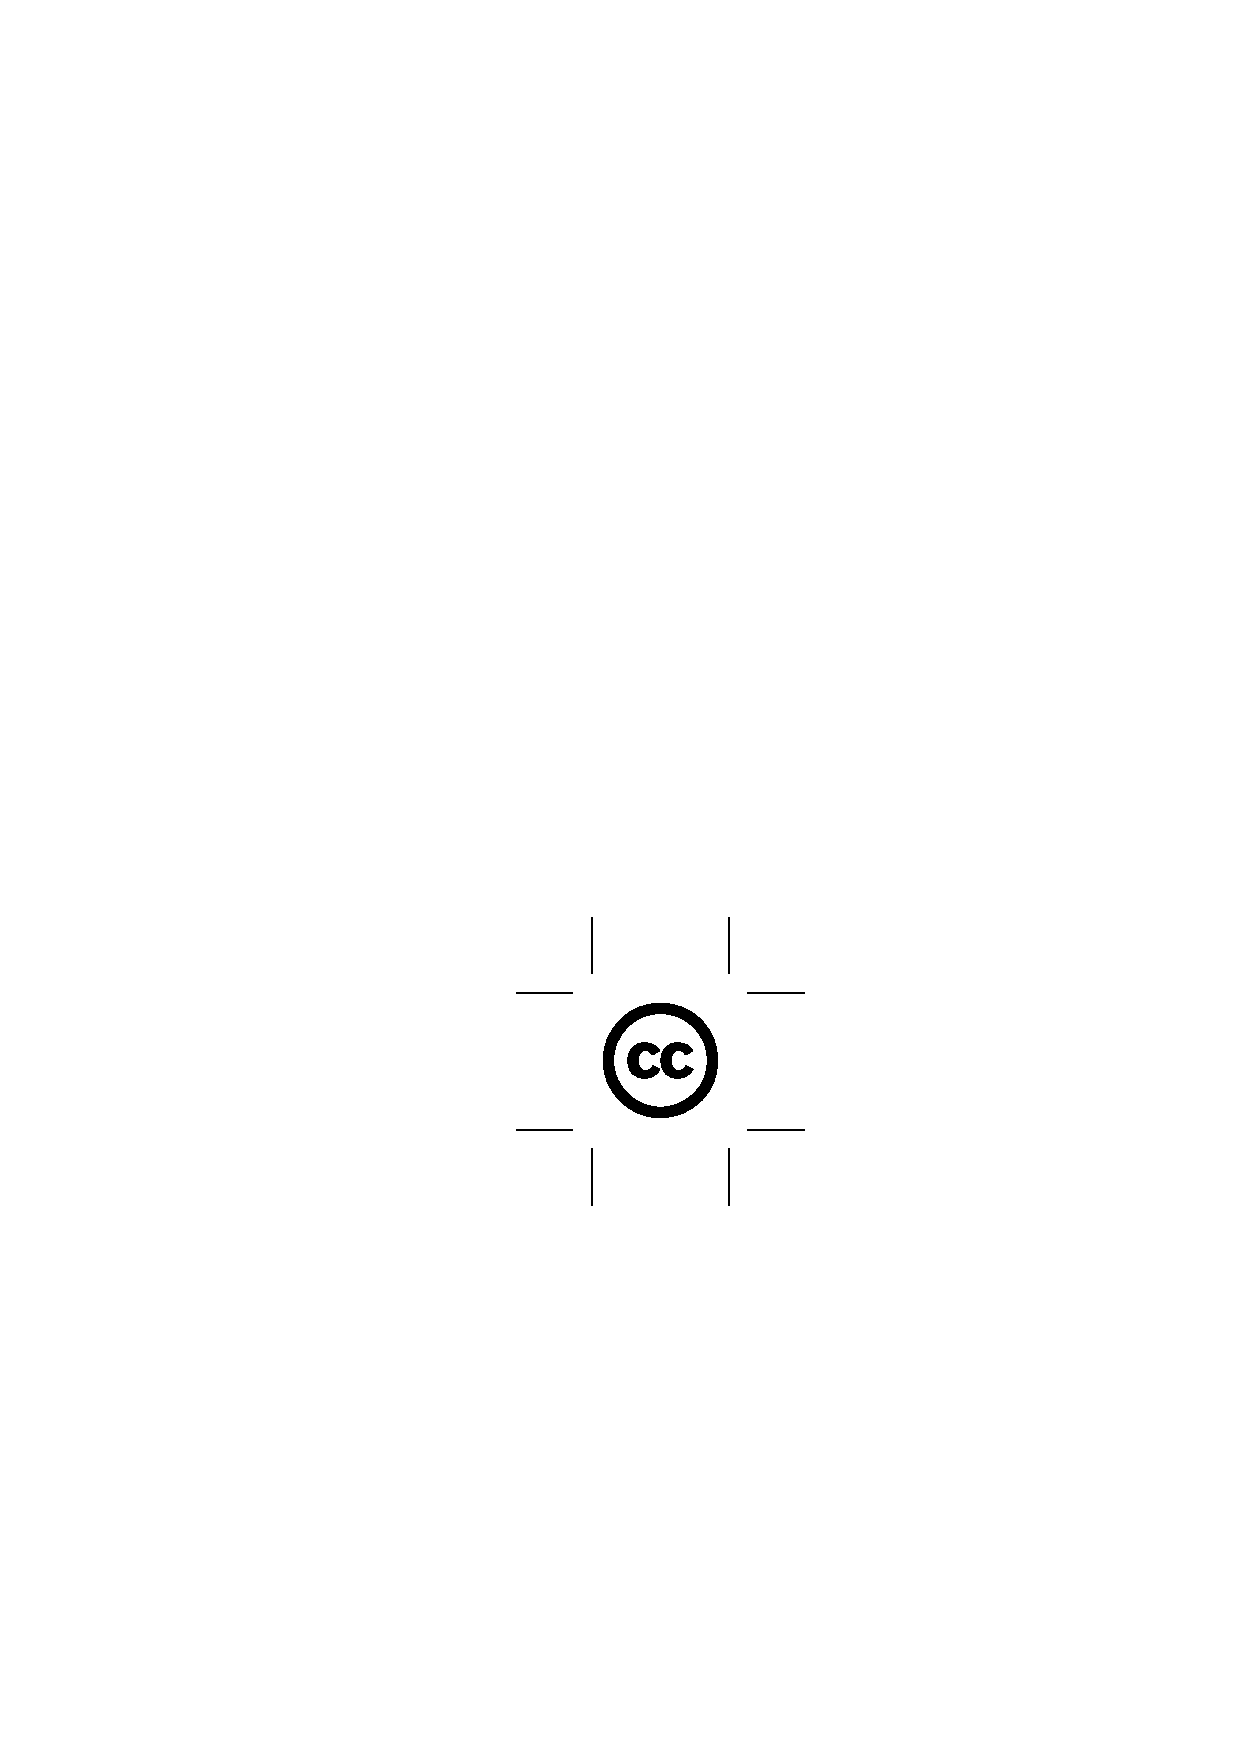
\includegraphics[height=4ex]{logos/creativecommons/cc}
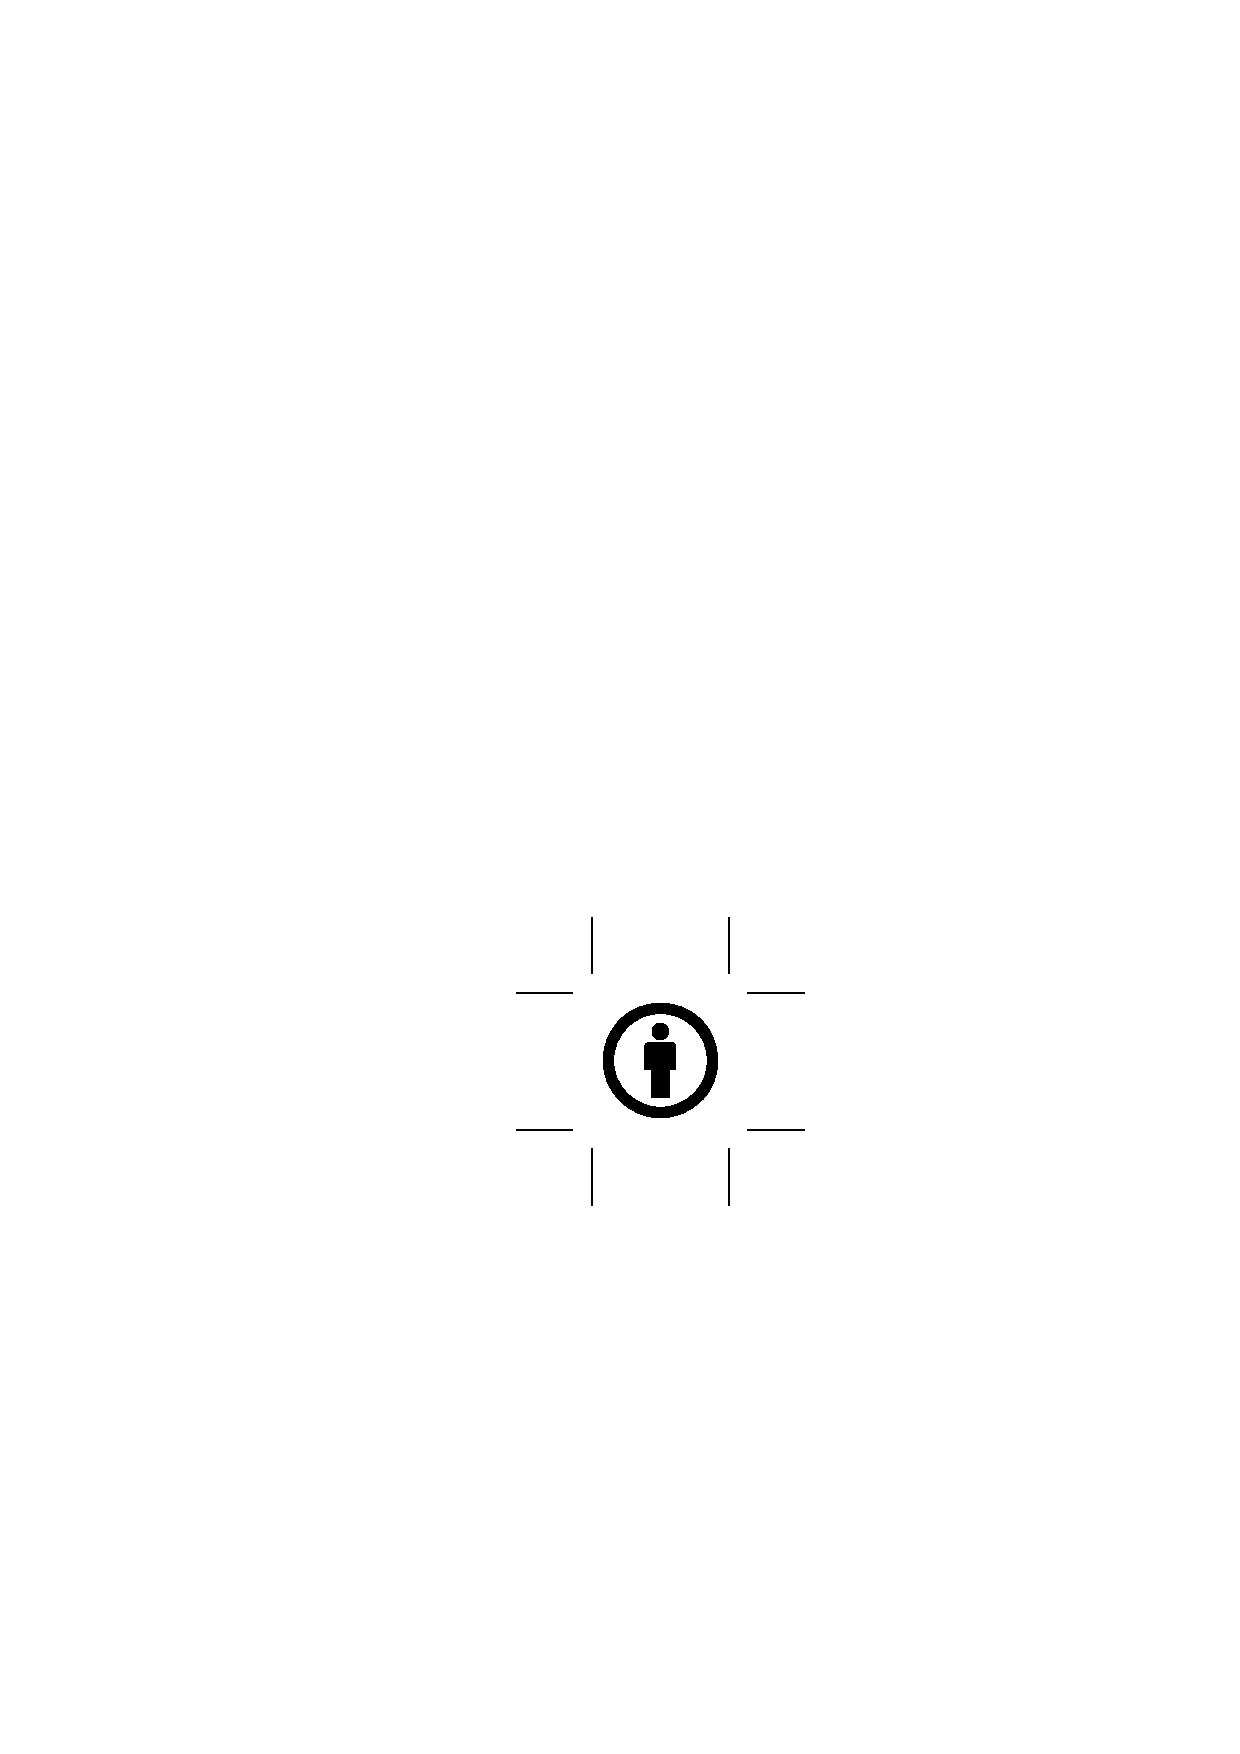
\includegraphics[height=4ex]{logos/creativecommons/by}
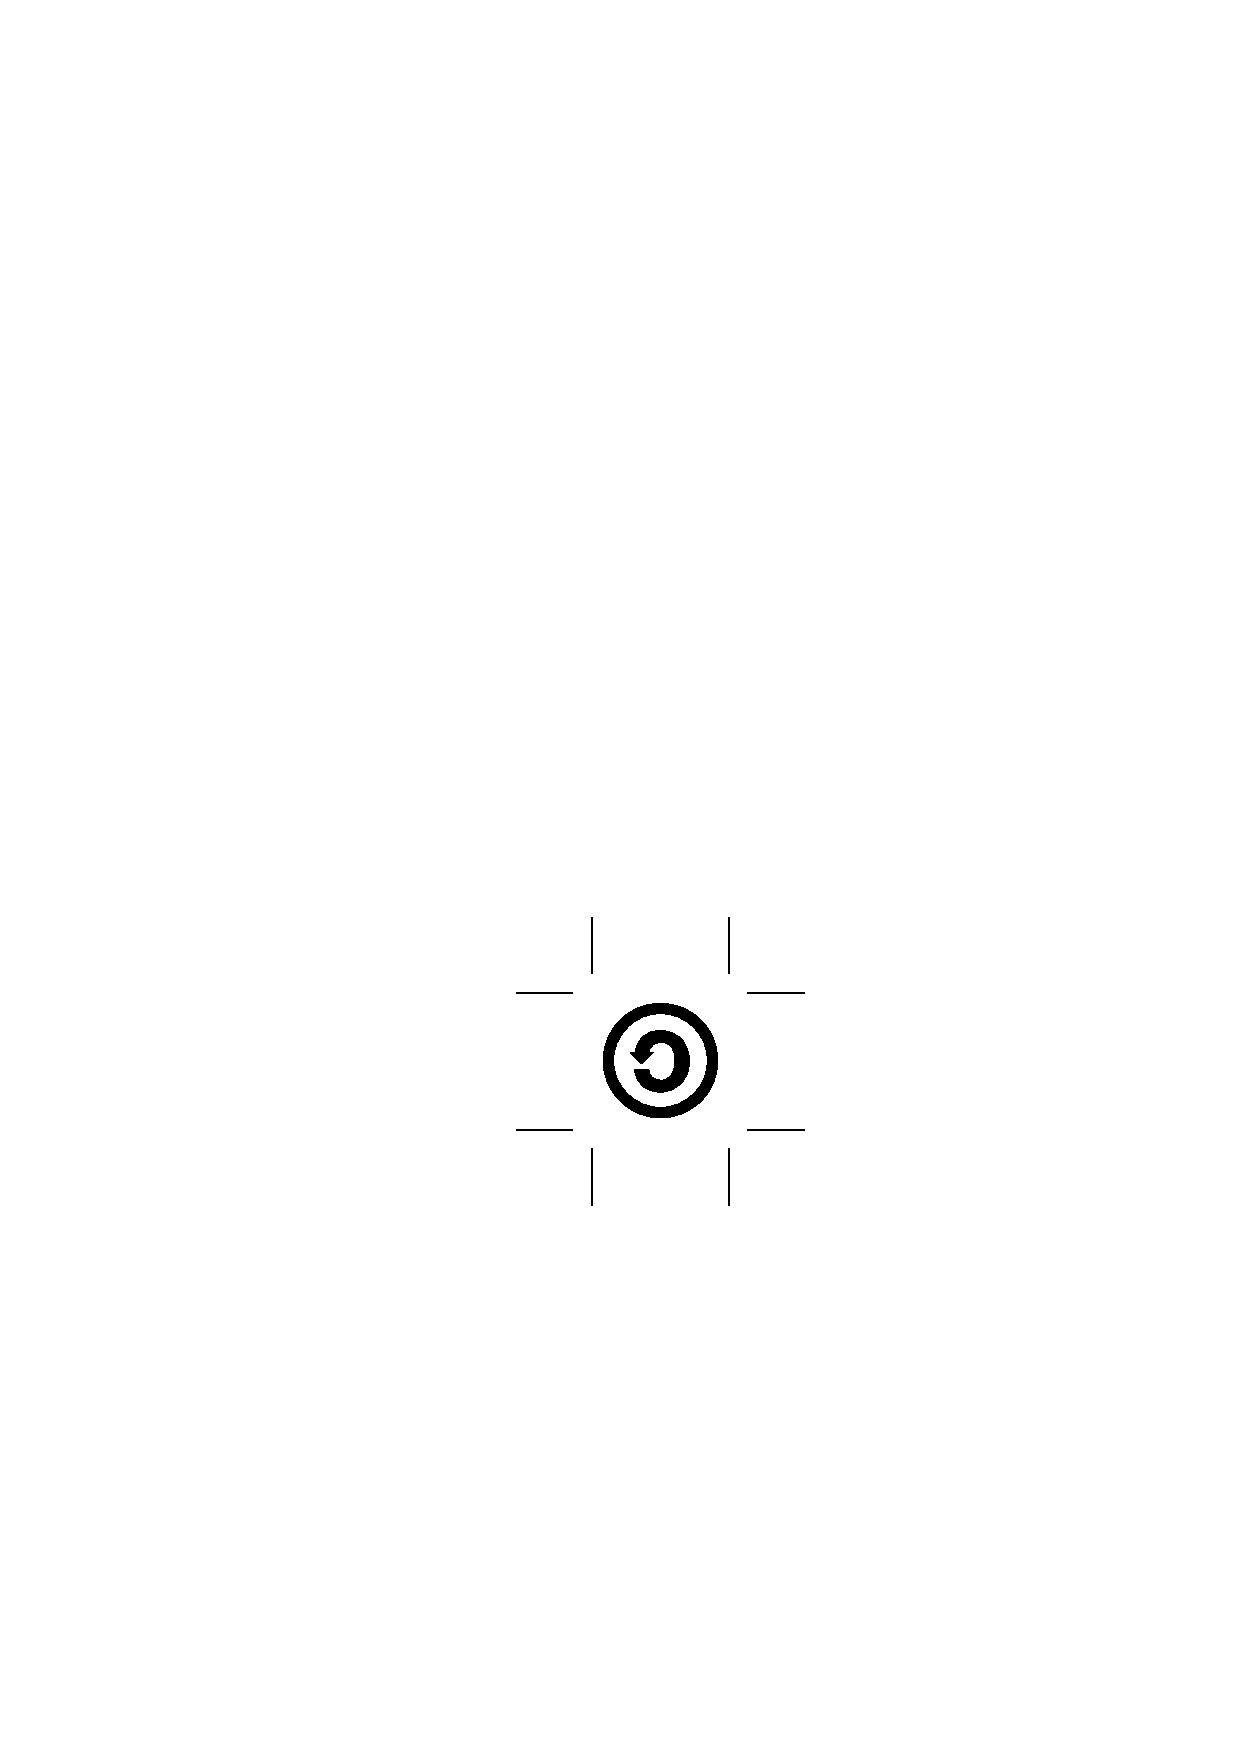
\includegraphics[height=4ex]{logos/creativecommons/sa}
% 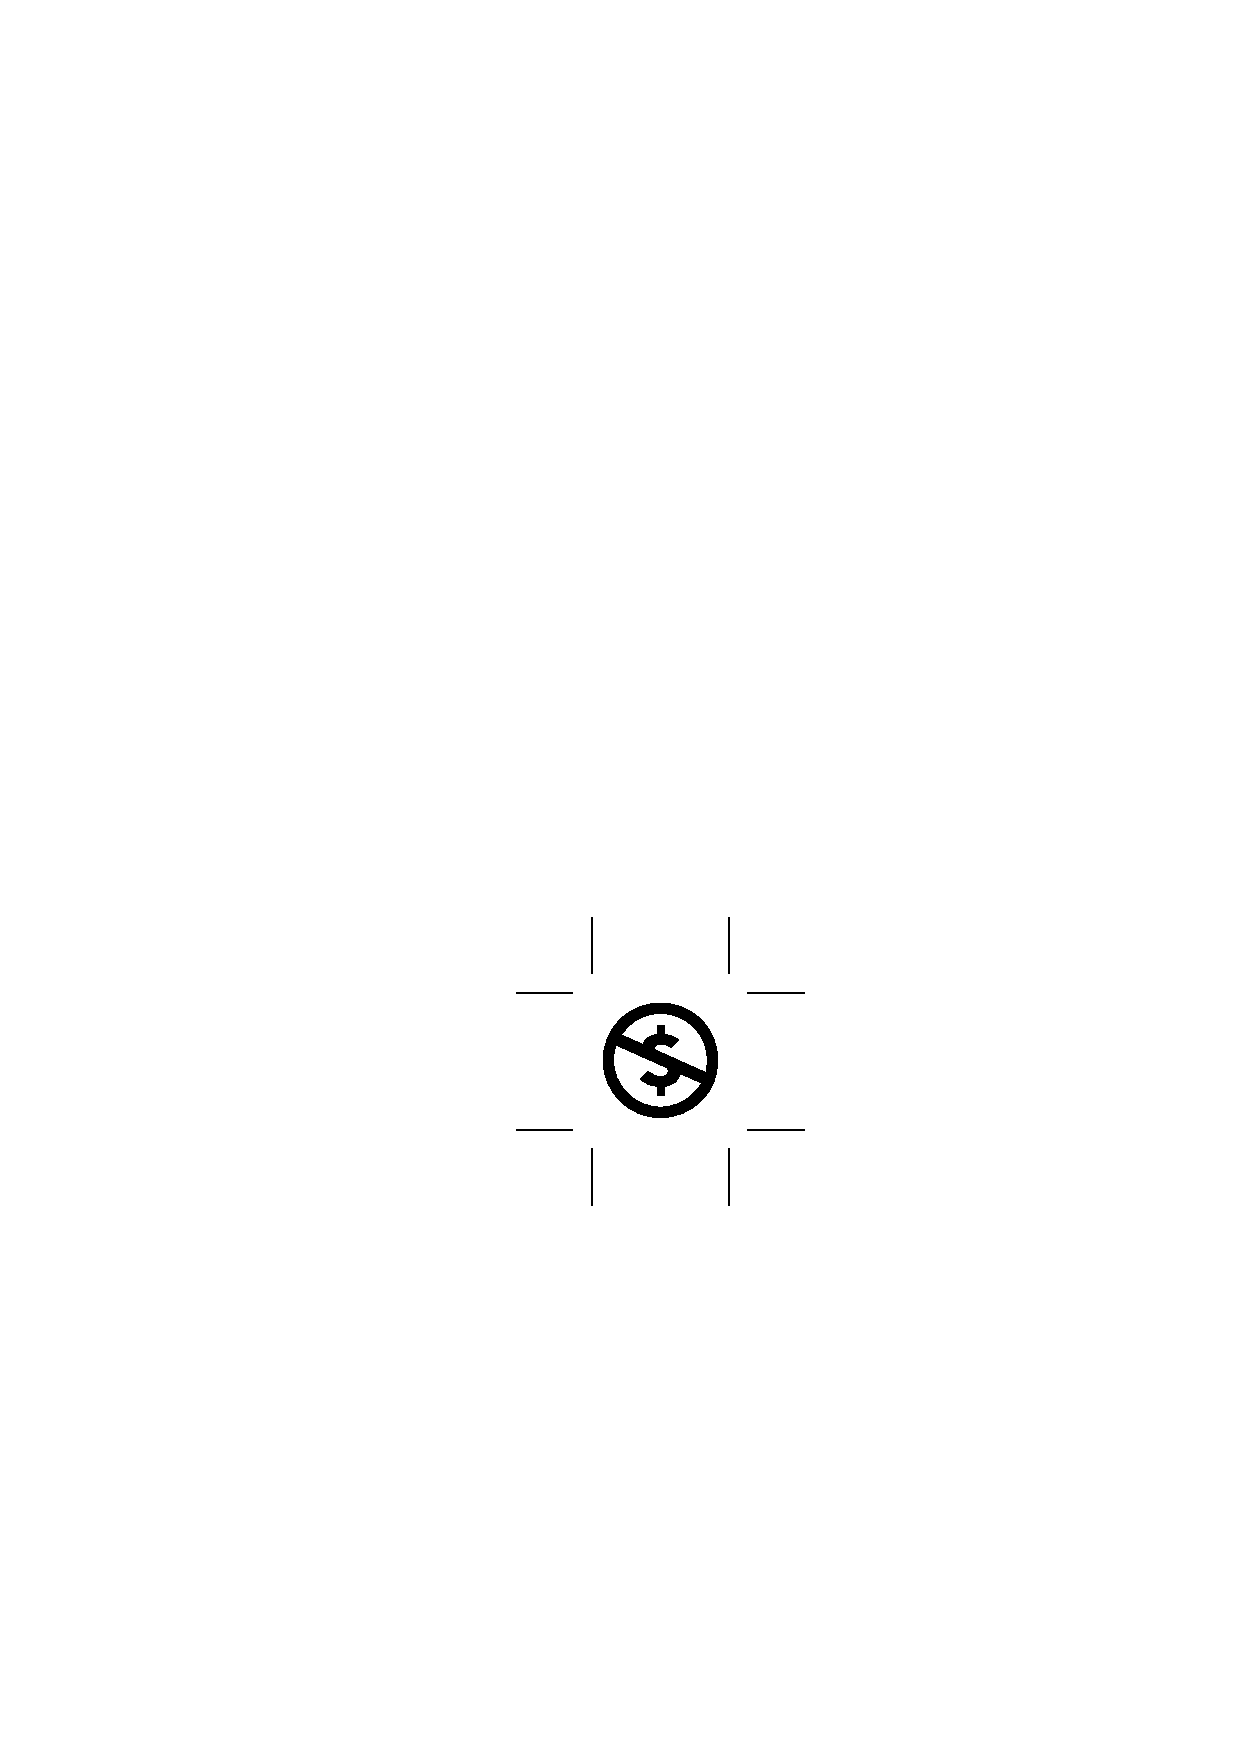
\includegraphics[height=4ex]{logos/creativecommons/nc}
% 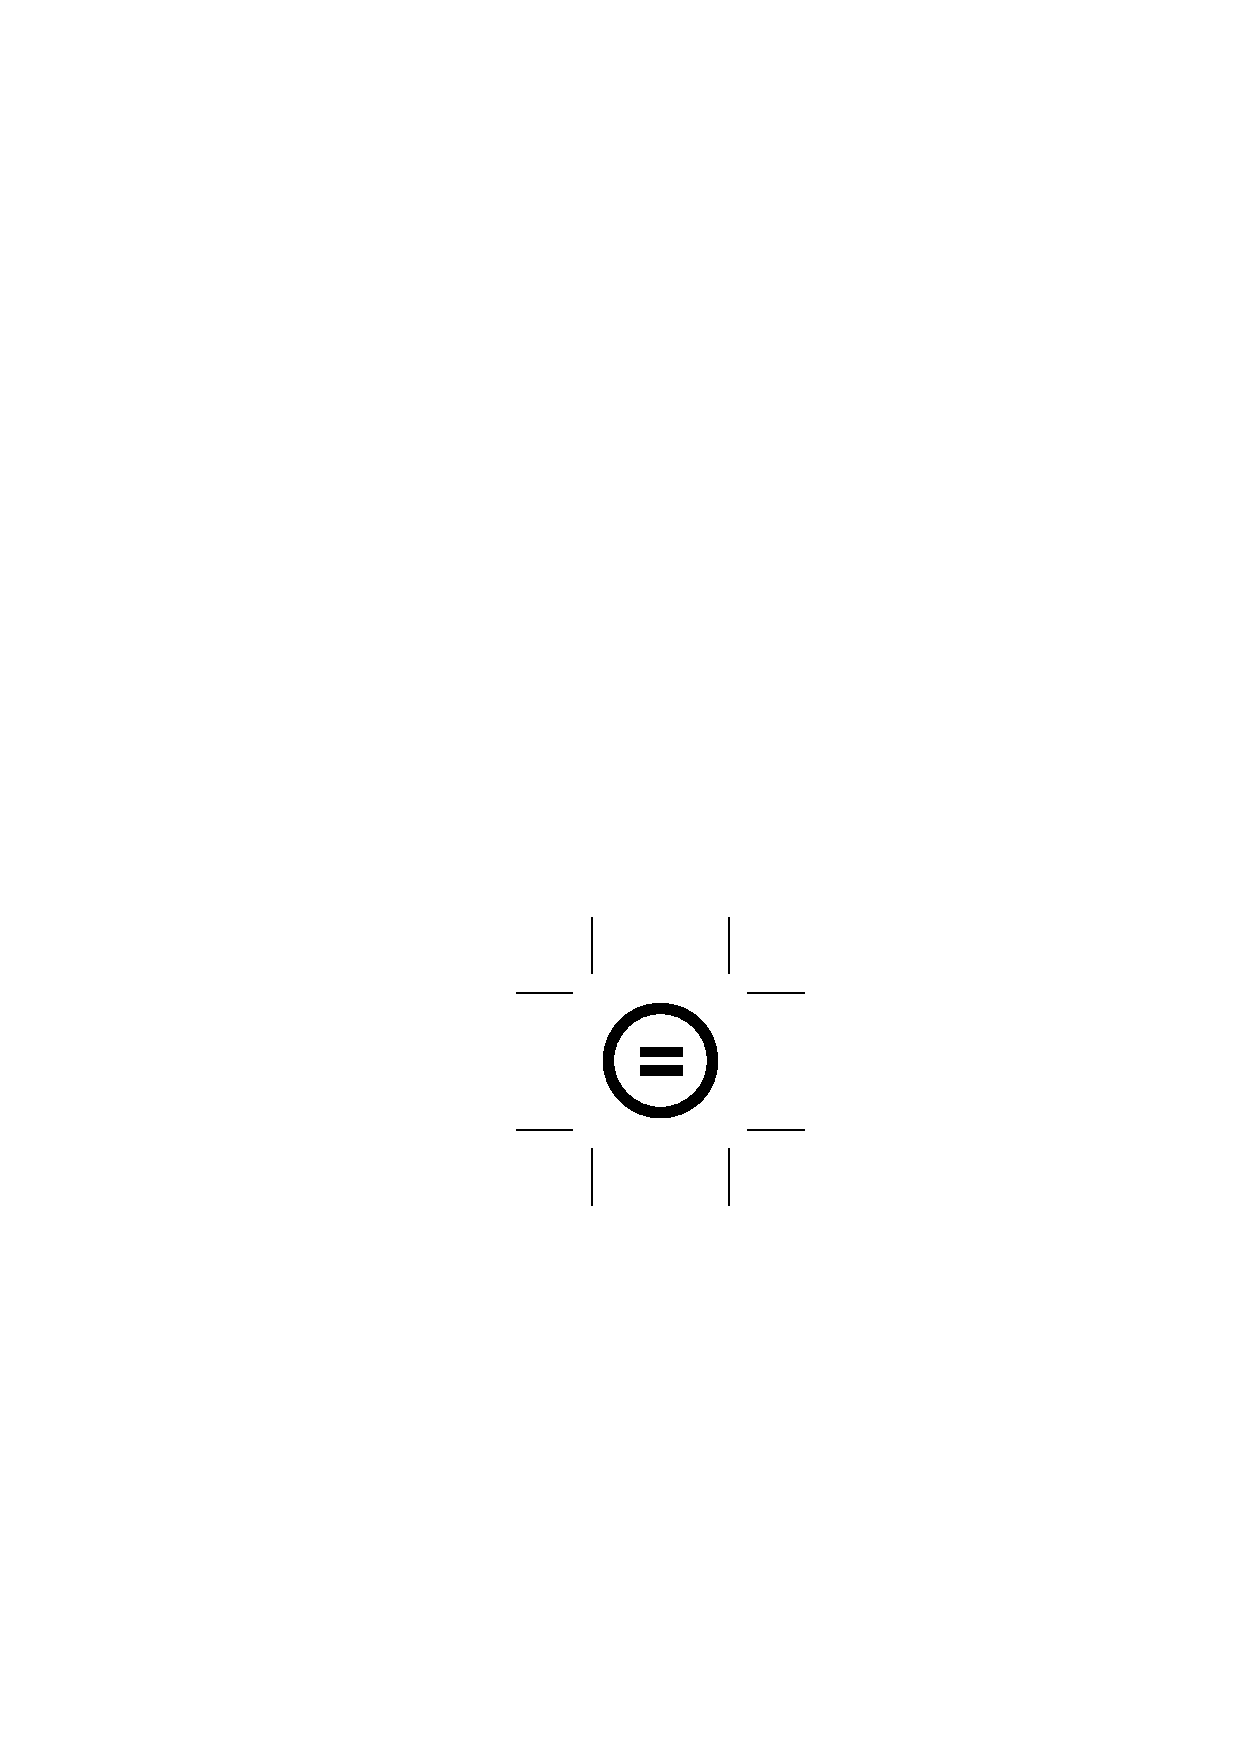
\includegraphics[height=4ex]{logos/creativecommons/nd}


\smallskip

\noindent%
Veröffentlicht unter \emph{CC BY-SA 4.0 International}
\emph{(Namensnennung -- Weitergabe unter gleichen Bedingungen)} \\
\url{https://creativecommons.org/licenses/by-sa/4.0/deed.de}

\end{otherlanguage}

\smallskip

\noindent%
Licensed under \emph{CC BY-SA 4.0 International}
\emph{(Attribution-ShareAlike)} \\
\url{https://creativecommons.org/licenses/by-sa/4.0/deed.en}

	\cleardoublepage% !TeX root = ../Thesis.tex

%*******************************************************
% Dedication
%*******************************************************
\thispagestyle{empty}
\phantomsection
% -- TemplateKnob
%\addcontentsline{toc}{chapter}{\texorpdfstring{\tocEntry{Dedication}}{Dedication}}%
\pdfbookmark[0]{Dedication}{Dedication} % Create only PDF bookmark, but no TOC entry

\vspace*{3cm}

\begin{center}
    \emph{Ohana} means family. \\
    Family means nobody gets left behind, or forgotten. \\ \medskip
    --- Lilo \& Stitch
\end{center}

\medskip

\begin{center}
    Dedicated to the loving memory of Rudolf Miede. \\ \smallskip
    1939\,--\,2005
\end{center}

}{
	% !TeX root = ../Thesis.tex

%*******************************************************
% Titlepage
%*******************************************************
\pdfbookmark[0]{Cover}{cover}
\begin{titlepage}
    % -- TemplateKnob
    % if you want the titlepage to be centered, uncomment and
    % fine-tune the line below (KOMA classes environment)
    %\pdfbookmark[1]{\myTitle{}}{titlepage}

    \begin{addmargin}[-1cm]{\iftoggle{adrianstyle}{-2cm}{-3cm}}
    \begin{center}
        \large

        
\includegraphics[width=6cm]{logos/tud-logo-rgb}
        
        \vfill

        \begingroup
            \color{CTtitle}\spacedallcaps{\myTitle{}} \\ \bigskip
        \endgroup

        \vspace{2ex}

        \spacedlowsmallcaps{\myName{}}

        \vfill

        \myDegree{}

        \vspace{2ex}

        \myTime{}

        \vfill

        \myDepartment{} \\
        \myFaculty{} \\
        \myUni{}

        \vfill

        
\includegraphics[width=5cm]{logos/seemoo-logo-rgb}
    \end{center}
    \end{addmargin}
\end{titlepage}

	% !TeX root = ../Thesis.tex

\thispagestyle{empty}

\ \vfill

\noindent%
\myName{}, \emph{\myTitle{}}, \myDegree, \myUni{}, \myYearPublication{}.

\bigskip

\noindent\myThesiscode{} \\
Date of submission: \myTime{}

\bigskip

\noindent\begin{tabular}{@{}l@{~}l@{}}
Advisor: & \myProf{} \\
Supervisor: & \mySupervisor{} \\
\end{tabular}

\bigskip

\noindent%
\myDepartment{} \\
\myFaculty{} \\
\myUni{}


% -- TemplateKnob
% \bigskip

% \noindent%
%% Choose the logos based on your desired CC license.
% 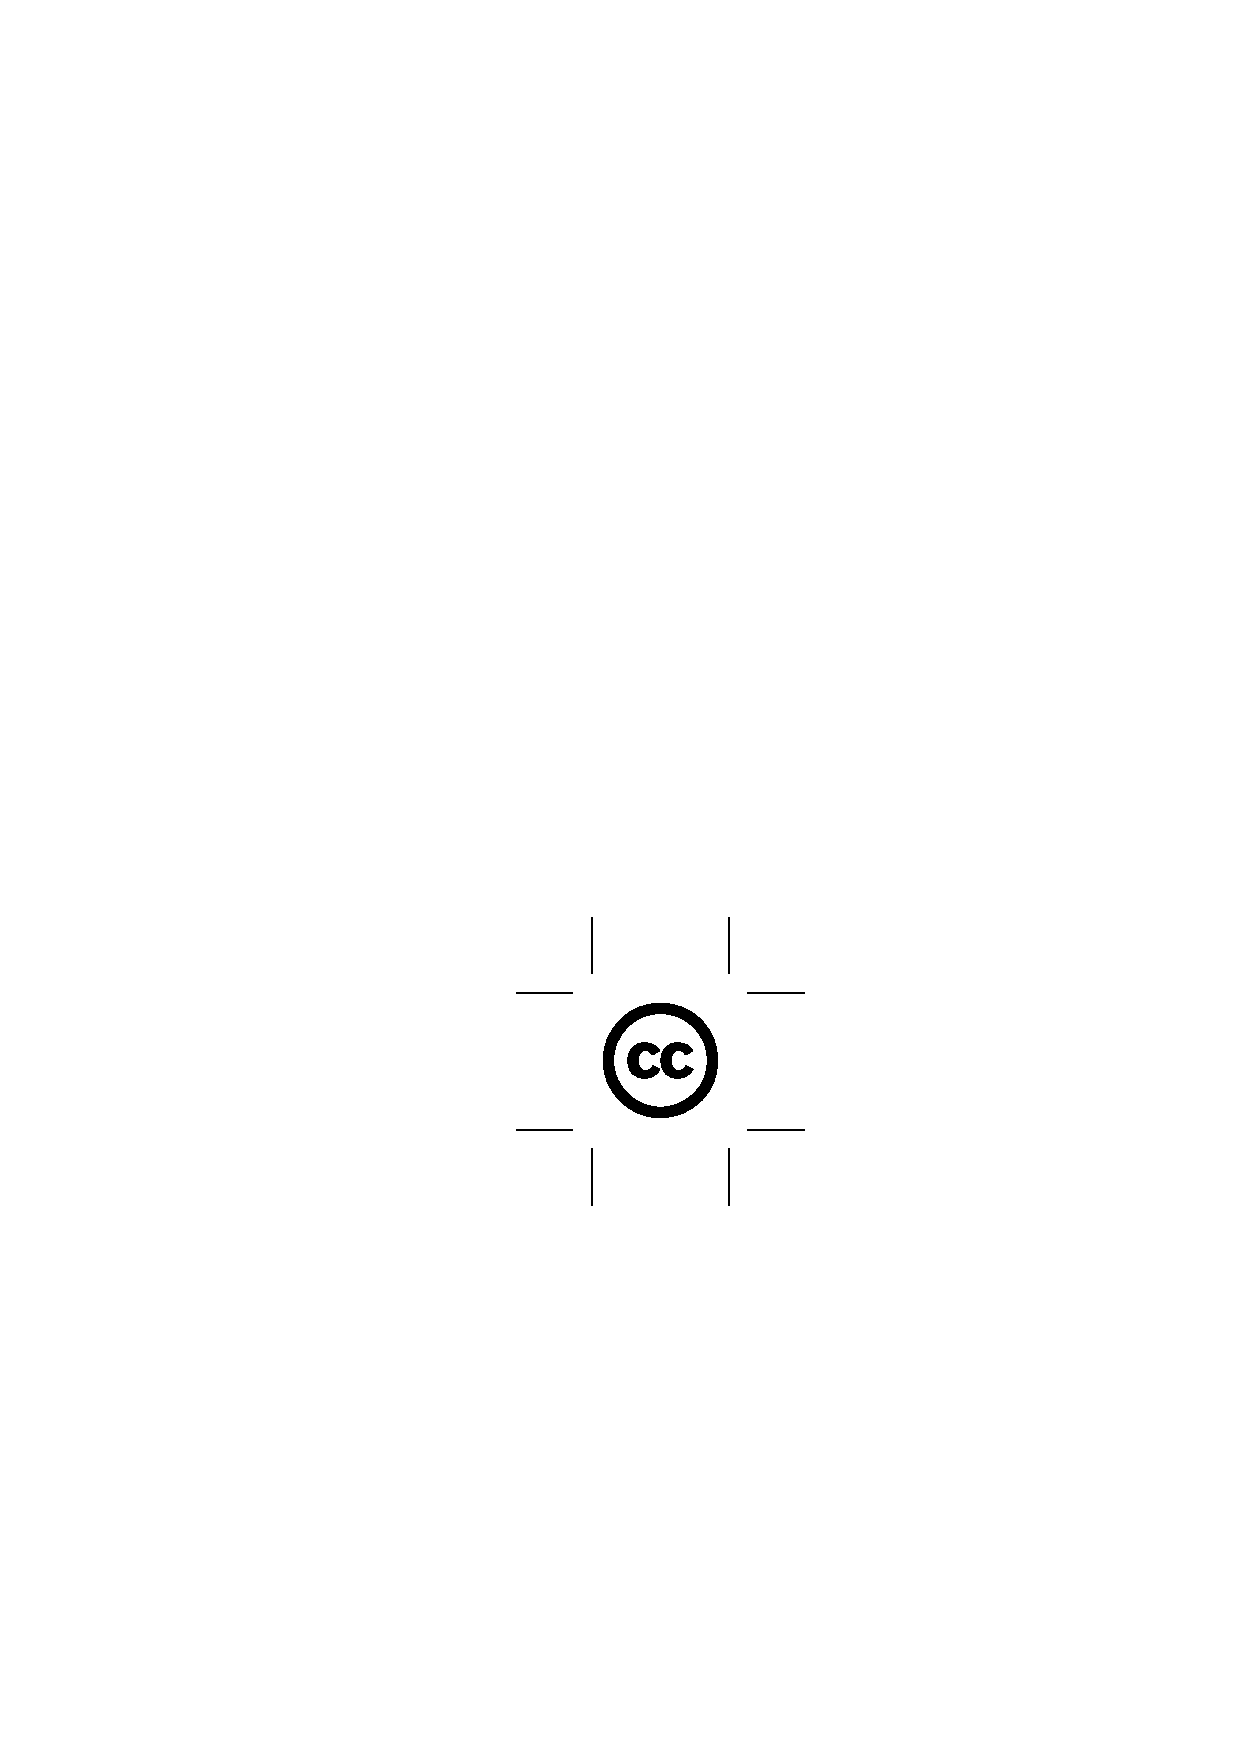
\includegraphics[height=4ex]{logos/creativecommons/cc}
% 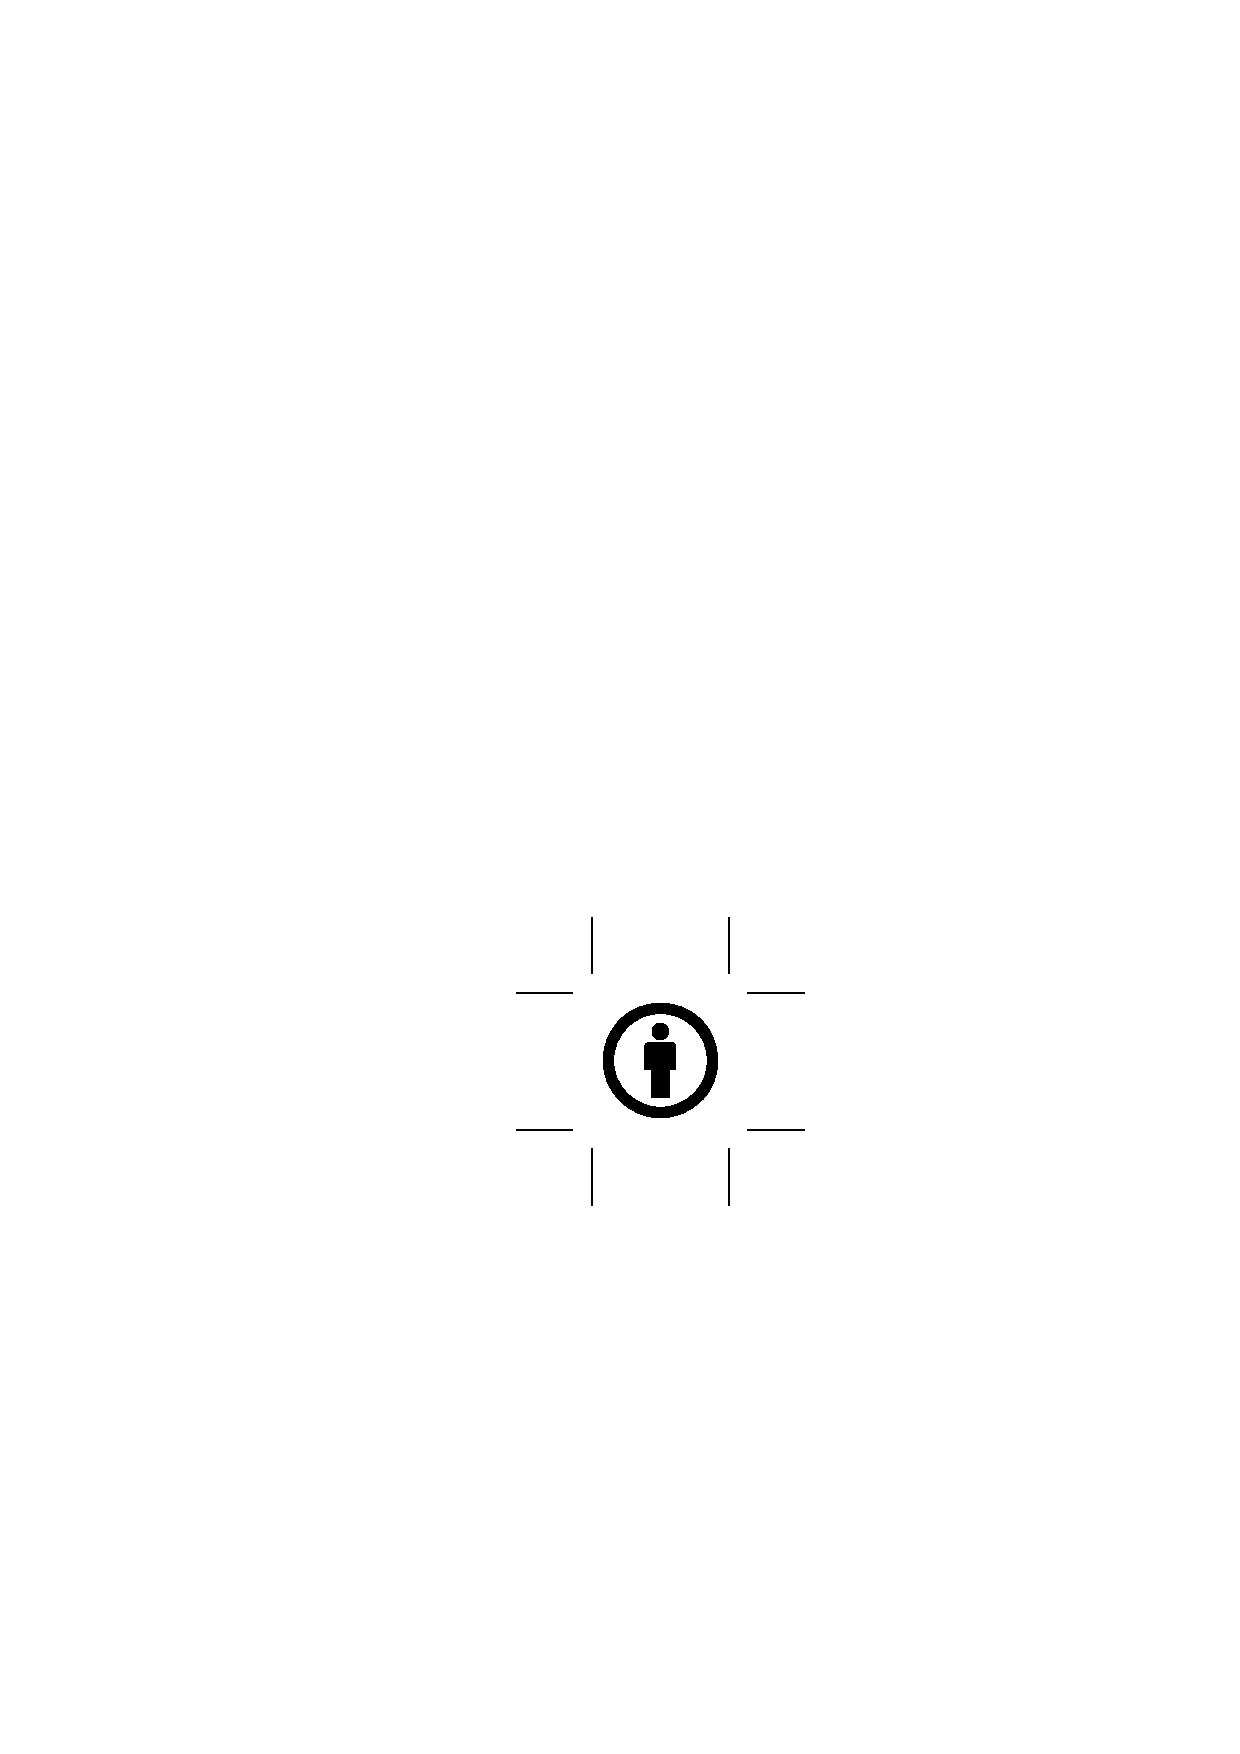
\includegraphics[height=4ex]{logos/creativecommons/by}
% 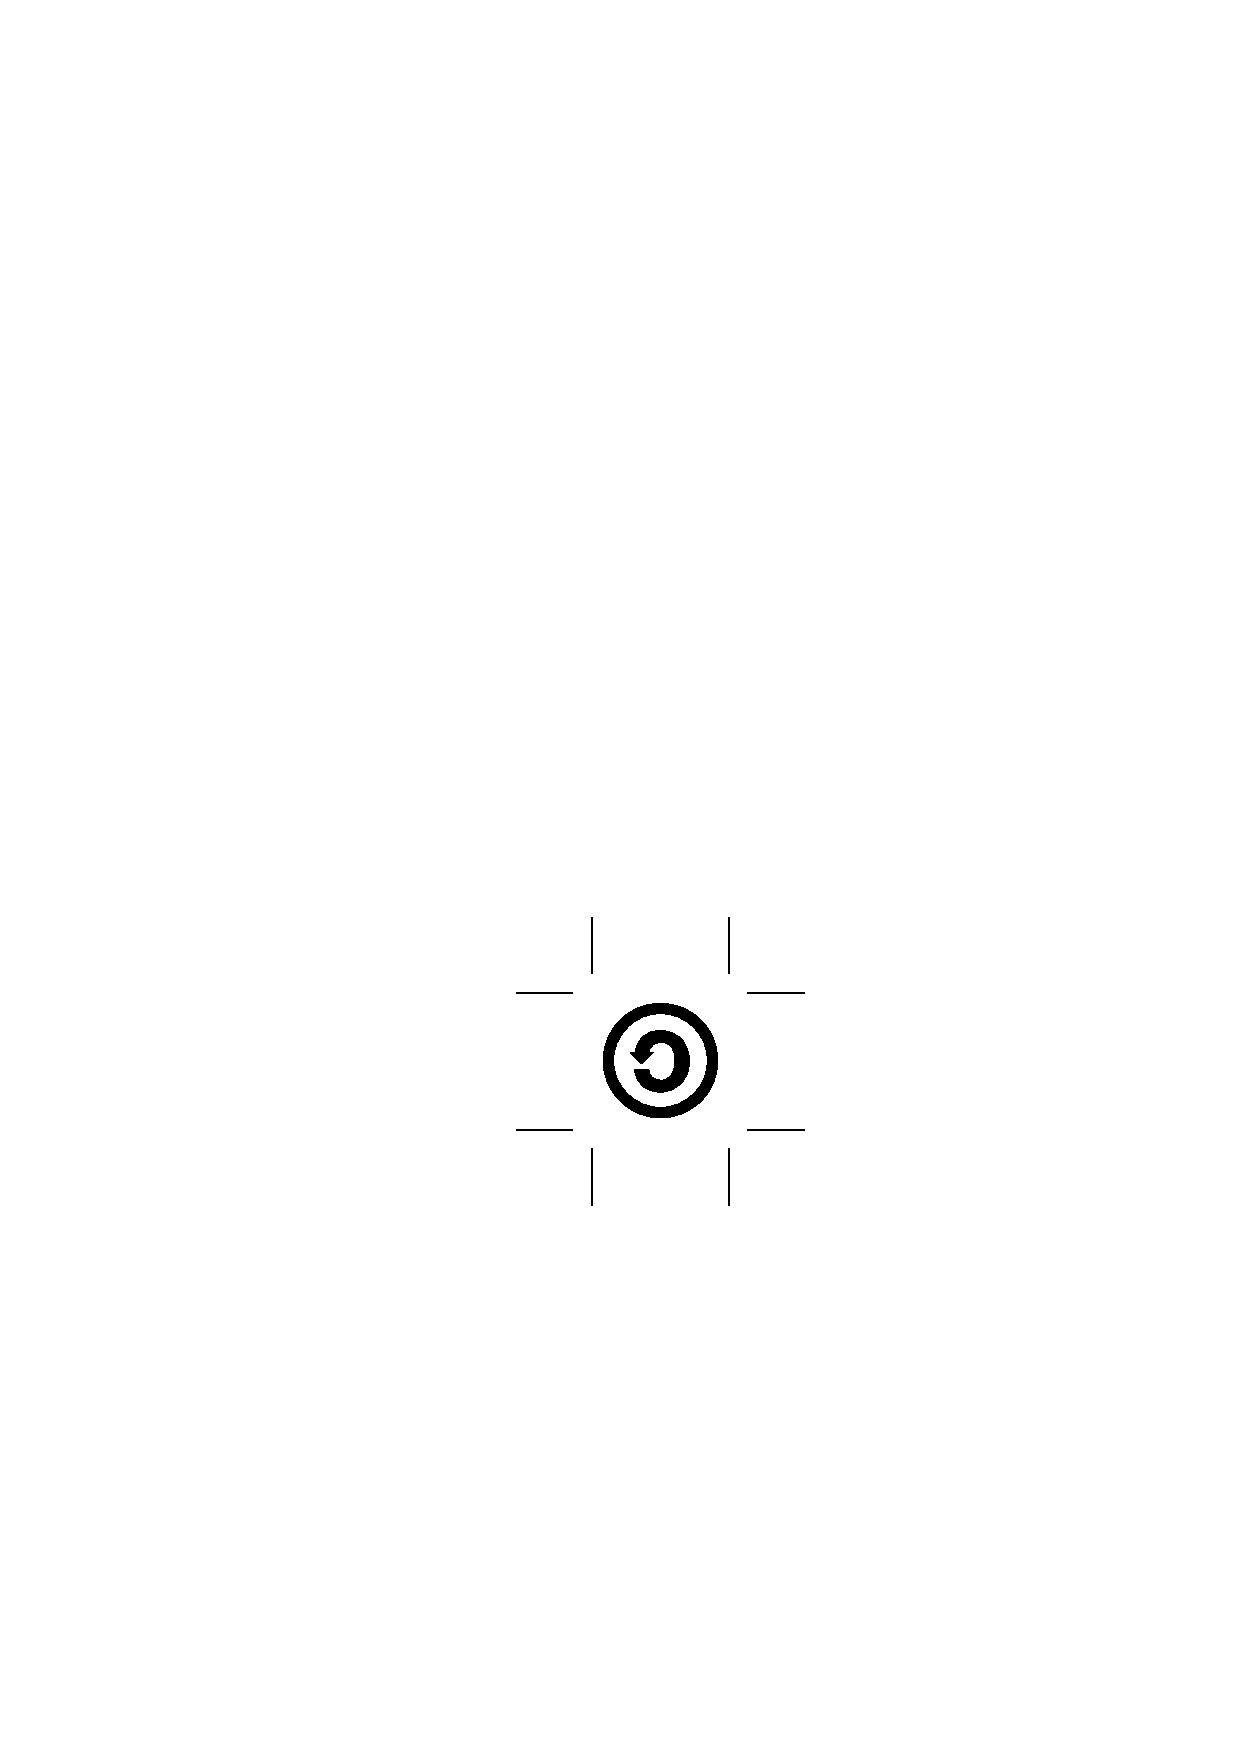
\includegraphics[height=4ex]{logos/creativecommons/sa}
%% 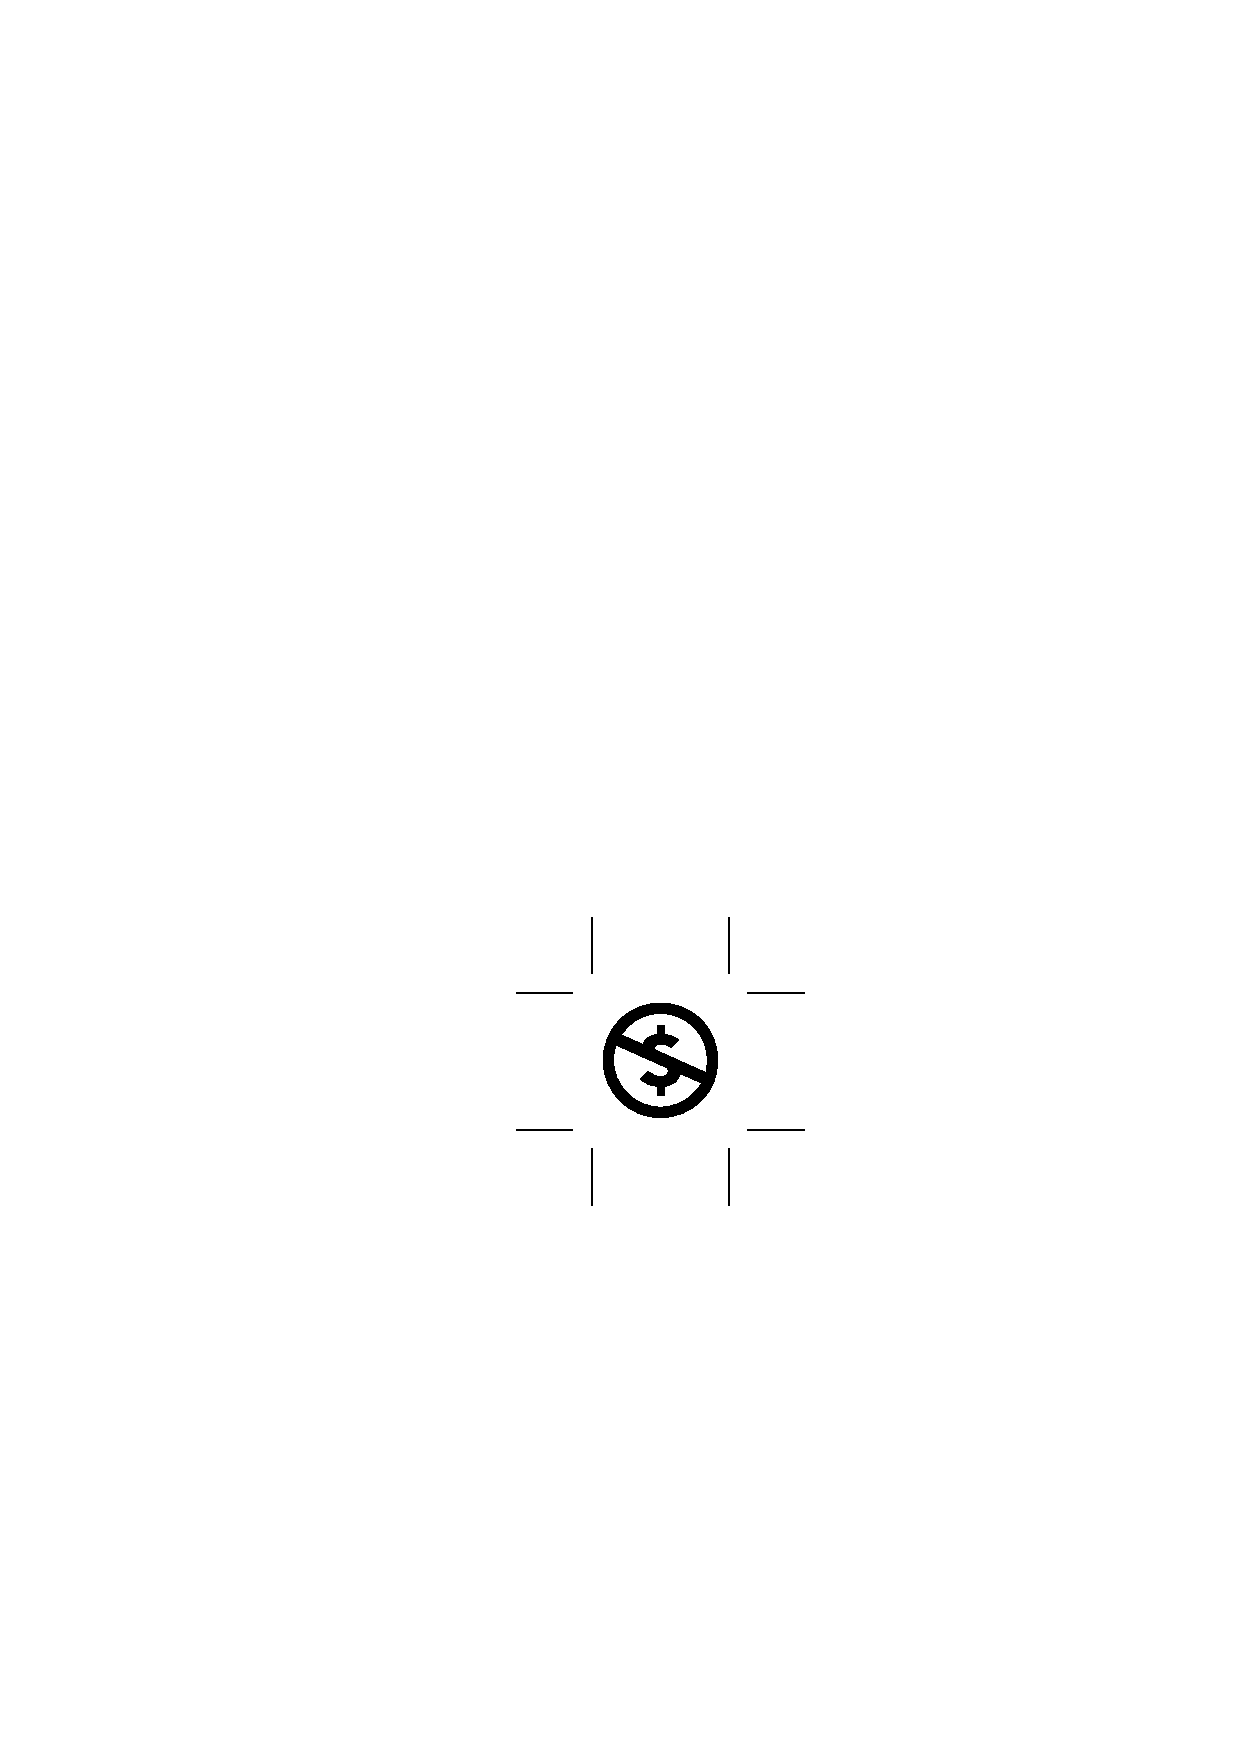
\includegraphics[height=4ex]{logos/creativecommons/nc}
%% 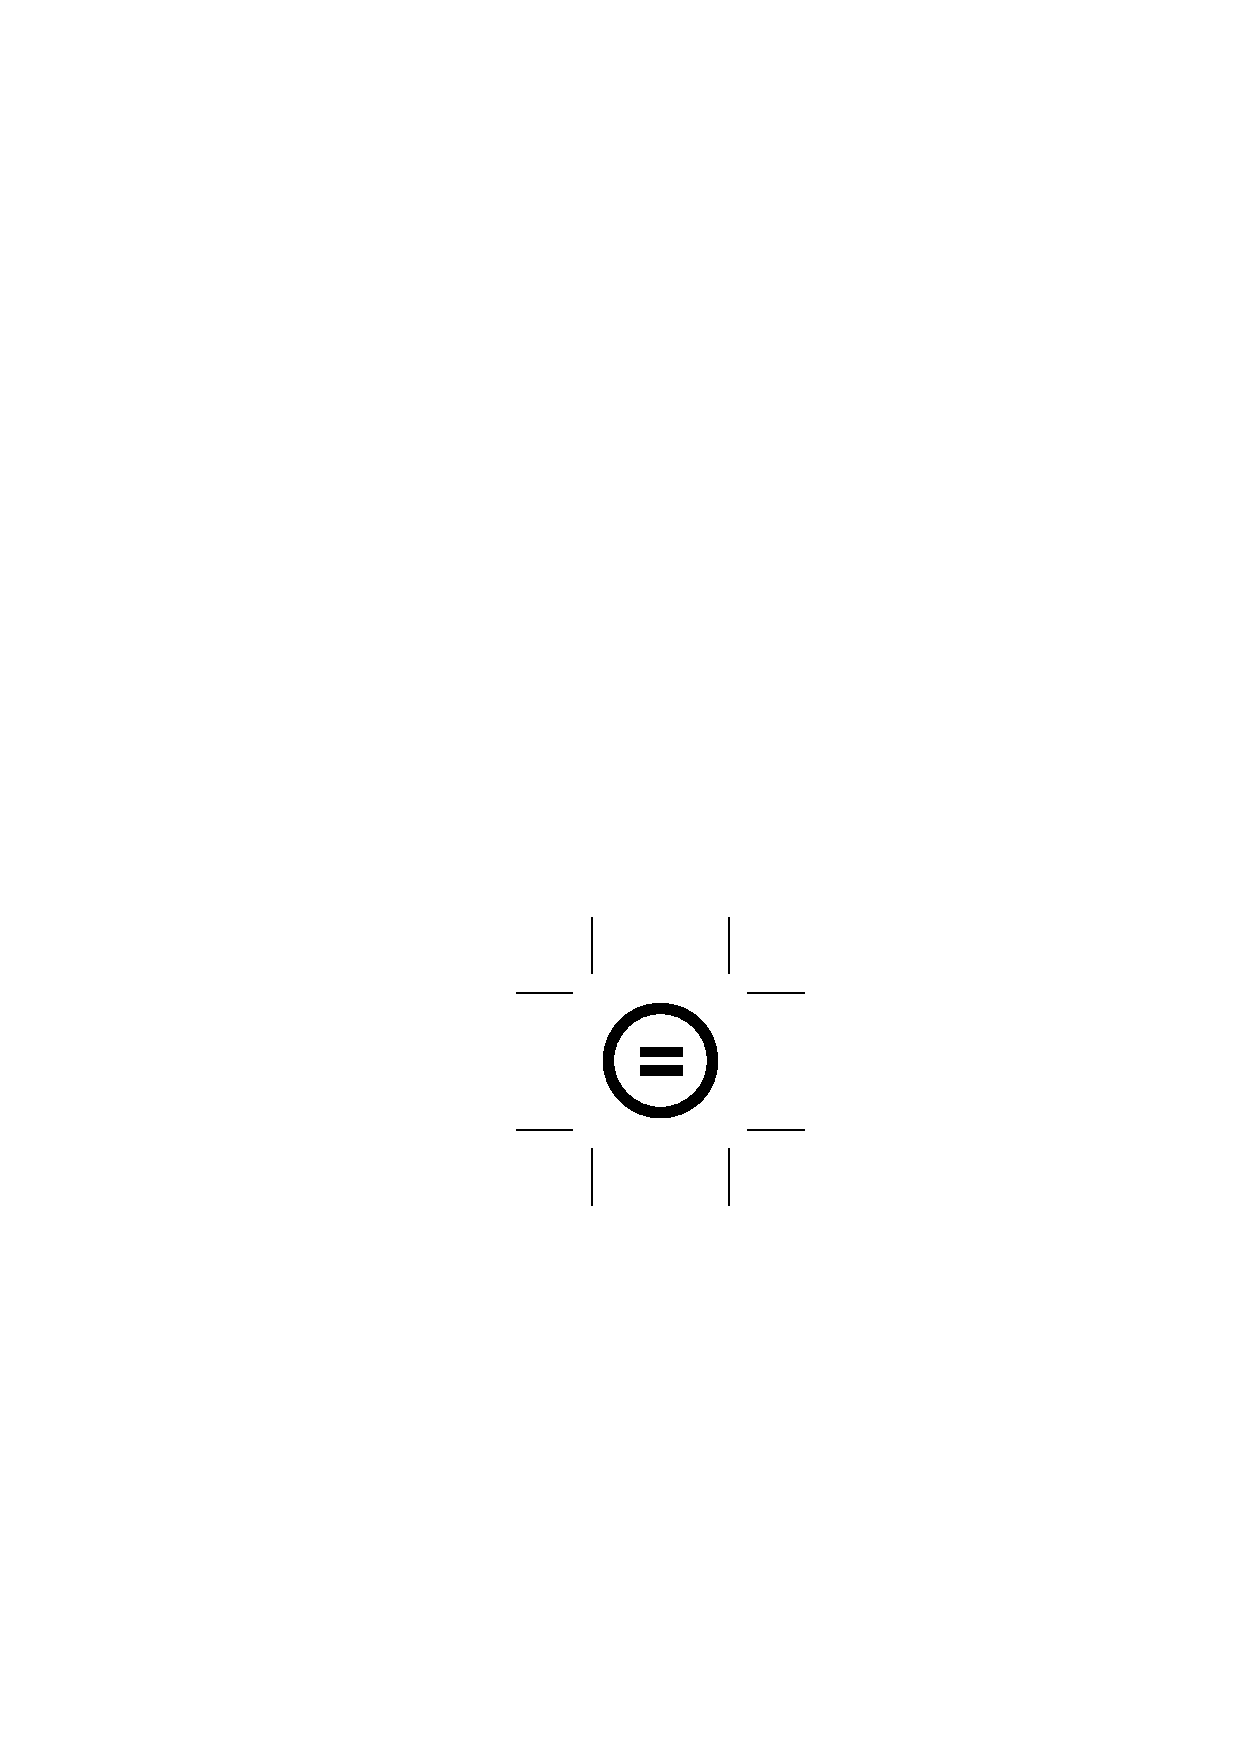
\includegraphics[height=4ex]{logos/creativecommons/nd}

% \smallskip

% \begin{otherlanguage}{ngerman}

% \noindent%
% Veröffentlicht unter \emph{CC BY-SA 4.0 International}
% \emph{(Namensnennung -- Weitergabe unter gleichen Bedingungen)} \\
% \url{https://creativecommons.org/licenses/by-sa/4.0/deed.de}

% \end{otherlanguage}

% \smallskip

% \noindent%
% Licensed under \emph{CC BY-SA 4.0 International}
% \emph{(Attribution-ShareAlike)} \\
% \url{https://creativecommons.org/licenses/by-sa/4.0/deed.en}

}

\cleardoublepage% !TeX root = ../Thesis.tex

%*******************************************************
% Abstract
%*******************************************************
\begingroup
\let\clearpage\relax
\let\cleardoublepage\relax
\let\cleardoublepage\relax

\chapterExtra{Abstract}

\vfill

\begin{otherlanguage}{ngerman}
\chapterExtra{Zusammenfassung}
\end{otherlanguage}

\endgroup

\vfill

\cleardoublepage% !TeX root = ../Thesis.tex

%*******************************************************
% Acknowledgments
%*******************************************************
\bigskip

\begingroup
\let\clearpage\relax
\let\cleardoublepage\relax
\let\cleardoublepage\relax

\chapterExtra{Acknowledgments}
{\slshape 
I would like to express my deepest gratitude to my parents and my family for supporting me in all the years of my studies and also while writing this thesis.

\bigskip

Special thanks for giving helpful advice while writing this thesis goes to Prof. Matthias Hollick and Nils Rollshausen.

\bigskip

Furthermore, I especially thank Nils Rollshausen for proofreading my thesis.
}

\endgroup

\cleardoublepage% !TeX root = ../Thesis.tex

%*******************************************************
% Table of Contents
%*******************************************************
\pagestyle{scrheadings}

\pdfbookmark[0]{\contentsname}{tableofcontents}
\setcounter{tocdepth}{2} % <-- 2 includes up to subsections in the ToC
\setcounter{secnumdepth}{3} % <-- 3 numbers up to subsubsections
\manualmark
\markboth{\spacedlowsmallcaps{\contentsname}}{\spacedlowsmallcaps{\contentsname}}
\tableofcontents
\automark[section]{chapter}
\renewcommand{\chaptermark}[1]{\markboth{\spacedlowsmallcaps{#1}}{\spacedlowsmallcaps{#1}}}
\renewcommand{\sectionmark}[1]{\markright{\textsc{\thesection}\enspace\spacedlowsmallcaps{#1}}}
%*******************************************************
% List of Figures and of the Tables
%*******************************************************
\clearpage
% -- TemplateKnob
% Uncomment this line if your lists should not have any
% headlines with section name and page number
% \pagestyle{empty}
\begingroup
    \let\clearpage\relax
    \let\cleardoublepage\relax
    %*******************************************************
    % List of Figures
    %*******************************************************
    \phantomsection
    \addcontentsline{toc}{chapter}{\texorpdfstring{\tocEntry{\listfigurename}}{\listfigurename}}
    \listoffigures

    \vspace{8ex}

    %*******************************************************
    % List of Tables
    %*******************************************************
    \phantomsection
    \addcontentsline{toc}{chapter}{\texorpdfstring{\tocEntry{\listtablename}}{\listtablename}}
    \listoftables

    \vspace{8ex}
    % \newpage

    %*******************************************************
    % List of Listings
    %*******************************************************
    \phantomsection
    \addcontentsline{toc}{chapter}{\texorpdfstring{\tocEntry{\lstlistlistingname}}{\lstlistlistingname}}
    \lstlistoflistings

    \vspace{8ex}

    %*******************************************************
    % Acronyms
    %*******************************************************
    \phantomsection
    \addcontentsline{toc}{chapter}{\texorpdfstring{\tocEntry{Acronyms}}{Acronyms}}
    \printglossary[type=\acronymtype]

\endgroup

\iftoggle{phd}{
	\begin{refsection}[own] % use numbering of list of publications
	\cleardoublepage% !TeX root = ../Thesis.tex

%*******************************************************
% Publications
%*******************************************************
\chapterExtra{List of Publications}
\label{ch:AuthorPublications}

During the course of writing this thesis, I co-authored several papers and articles that I list below.

\nocite{*} % print all references


\section*{Journal and Magazine Articles}

{\small\printbibliography[heading=none,type=article,notkeyword=underreview]}


\section*{Conference and Workshop Papers}

{\small\printbibliography[heading=none,type=inproceedings,notkeyword=underreview,notkeyword=posterdemo]}


\section*{Posters and Demonstrators}

{\small\printbibliography[heading=none,type=inproceedings,notkeyword=underreview,keyword=posterdemo]}


\section*{Under Peer Review}

{\small\printbibliography[heading=none,type=article,keyword=underreview]}


\label{ch:AuthorPublicationsEnd}

	\cleardoublepage% !TeX root = ../Thesis.tex

%*******************************************************
\chapterExtra{Collaborations and My Contribution}
%*******************************************************
\label{ch:Collaborations}

% From Daniel Steinmetzer's dissertation
Systematically investigating a technical research topic and engineering the required tools is a demanding and interdisciplinary process. Most achievements could never evolve without collaborations in which colleagues and international partners integrated their intellectual forces. When working in teams, accounting particular contributions and components of the resulting publications to individual collaborators becomes almost impossible. This situation also applies to several contents of this thesis, which arise from collaborations, thus, cover joint contributions. Many of these collaborations persisted even longer than the research projects and became a long-term strategic partnership.
In our previous publications, all authors contributed by discussing ideas and debating on results throughout the whole project duration. Each of them has particular strengths that sometimes appear invisible. For this reason, I explicitly state and acknowledge---where possible---the contributions of my collaborators in the following.

% From Milan Stute's dissertation
In the following, I detail the contributions of my co-authors and myself per chapter. In addition, I follow the regulations of the \myFaculty{} at \myUni{} and give an account of the parts that include verbatim or revised fragments of previous publications that form this thesis as indicated in the preceding list of publications.\footnote{References in this chapter refer to my list of publications given on \cpagerefrange*{ch:AuthorPublications}{ch:AuthorPublicationsEnd}.}

\sloppy

\Cref{ch:introduction,ch:relatedwork} collate the contributions, background, and related work sections of the core papers that form this thesis~\cite{Stute2018a,Stute2020}.

% etc etc etc

\fussy

\label{ch:CollaborationsEnd}
	\end{refsection}
}{}


% ------------------------------------------------------------------
% Mainmatter
% ------------------------------------------------------------------
\addtocounter{table}{-1} % otherwise starts counting from 2
\cleardoublepage
\pagestyle{scrheadings}
\pagenumbering{arabic}

% use \cleardoublepage here to avoid problems with pdfbookmark
\cleardoublepage
\iftoggle{parts}{
	\ctparttext{The first chapter of this part gives an introduction and a motivation to this thesis, followed by a presentation of related work found in the area of physical layer security. In the third chapter, we present some definitions and background information to make it easier for the reader to quickly understand the subsequent parts of this thesis.}
	\partExtra{Introduction}
}{}
% !TeX root = ../Thesis.tex

%************************************************
\chapter{Introduction}\label{ch:introduction}
%************************************************
\glsresetall % Resets all acronyms to not used

In today's digital age, sensitive information is constantly exchanged over the internet. Protecting our privacy and security is more important than ever. Although the platforms we use to communicate change frequently, one constant persists: Our communication is heavily text-based. This encompasses instant messaging, email, \gls{SMS}, social media, forums, blogs, and more.

In this thesis, we focus on what is likely the most sensitive use case: Instant messaging. People share deeply personal information in chat messages, such as their political beliefs, sexual orientation, religious views, or financial situation. As a result, mobile devices are frequent targets of attacks. Once an attacker gets hold of our communication, they can use it against us in various ways. This ranges from stalking in abusive relationships to evidence in legal proceedings.

One might think that modern instant messengers are equipped with sufficient security measures to protect our data, given the widespread use of technologies like \gls{E2EE} and \gls{2FA}. But most of these mechanisms primarily address remote attackers, overlooking the threat of a physically present attacker. This could be the partner in a relationship or a law enforcement officer. Currently, protection against this type of attacker is limited. Typical examples include local authentication methods, such as unlocking the messenger app with a fingerprint, or self-destructing messages that delete after a set timer. But these approaches come with significant drawbacks. The former can be bypassed easily by the attacker physically forcing the victim to unlock the app. The latter often does not provide the desired user experience for everyday life.

A promising solution is presented by steganography. This technique involves concealing information within an inconspicuous cover signal. Possible cover signals include digital images, audio, video, or - most notably in this context - natural language text. Natural language in particular is suitable as a cover signal because it is independent from any one communication medium~\cite{zieglerNeuralLinguisticSteganography2019}. This can be leveraged to embed a sensitive \textit{secret message} into a generic \textit{cover text} to be sent as chat message~\cite{zieglerNeuralLinguisticSteganography2019}. As a result, even a physically present attacker could be misled, protecting the victim from potential harm. This approach introduces a layer of security currently missing in popular instant messengers.

By implementing the core functionality of a chat app with built-in steganography on Android, we set the precedent for further research and development. Our app is called \gls{HiPS}\footnote{Source code is available at \url{https://github.com/tobiasvonderheidt/hips}.}. It runs a \gls{LLM} locally on the smartphone to generate the cover text for a given secret message and vice versa. As the scope of this thesis doesn't involve a server backend, users of our app can try the steganography in a demo conversation view. Furthermore, we offer a standalone functionality to use steganography with existing instant messengers by copy-pasting messages. This enables real-world users to protect themselves already today.

We implement steganography with two algorithms demonstrated in a project called Stegasuras~\cite{zieglerNeuralLinguisticSteganography2019}. Its modular architecture allows for future adaptations to which algorithms are used in each of the following steps:

\begin{enumerate}
    \item Convert the secret message from string to binary, compressing it in the process.
    \item Encrypt the secret message bits.
    \item Generate a cover text by completing a given context with the \gls{LLM}, thereby encoding the encrypted bits.
\end{enumerate}

The popular llama.cpp framework~\cite{gerganovGgerganovLlamacpp2024} is used to run \glspl{LLM} locally. This choice allows us to access a broad range of \glspl{LLM} readily available in the \lstinline|.gguf| file format on platforms like HuggingFace~\cite{huggingfaceModelsHuggingFace2025}. Adapting our implementation to different devices becomes as easy as swapping out the \gls{LLM}: We are able to deploy a small\footnote{Note that there is no clear definition when a language model is considered \textit{large}. For our purposes, any modern language model is called \gls{LLM}.} \gls{LLM} on an entry-level smartphone the same way we deploy a large \gls{LLM} on a flagship.

Overall, our app creates value and ensures its longevity by fulfilling the following requirements:

\begin{enumerate}
    \item Create a chat conversation between cover texts by generating them with a \gls{LLM}.
    \item Run the \gls{LLM} locally on an Android smartphone, i.e. don't require any internet connection for the steganography itself.
    \item Achieve acceptable performance on entry-level devices.
    \item Make the \gls{LLM} swappable.
\end{enumerate}

Lastly, we conducted a survey amongst students of TU Darmstadt to evaluate the plausibility of our cover texts in comparison to real chat conversations. This resulted in profound insights into the linguistics of chat messages and serves as a starting point for further optimizations of cover text quality. By creating a well-documented, easy-to-maintain implementation of text-based steganography on Android, we open up many opportunities for further research to be conducted at SEEMOO.

% !TeX root = ../Thesis.tex

%************************************************
\chapter{Background}\label{ch:background}
%************************************************
\glsresetall % Resets all acronyms to not used

To deepen our understanding for the underlying motivation of this thesis, we take a dive into the historical backgrounds of both steganography and \glspl{LLM}. Thereby, we deduct the requirements for our app.

\section{Steganography}
\label{sec:steganography}
To justify the relevance of steganography for the average user of instant messengers, we investigate its origins and involve some of today's politics. Then we formalize it and distinguish it from adjacent fields to lay the foundation our app is built upon.

\subsection{From physical to digital steganography}
\label{sec:fromPhysicalToDigitalSteganography}
The term "steganography" originates from ancient Greece and can be translated to "hidden writing"~\cite{kolataVeiledMessagesTerror2001,dembartEndUserHide2001}. Old Greek historian Herodotus documented it as early as 440 B.C.: Histiaeus, tyrant ruler of Miletus, was being held captive and wanted to send a message to his ally, Aristagoras. Since he had to bypass the guards of his enemies, the message had to be secret. He decided to shave the head of his most trusted slave, tattoo the message onto his scalp and wait for the hair to grow back before sending him on his way. With the message obscured, the slave would arrive at his destination, only for his hair to be shaved off again to read the secret message back~\cite{bennettLinguisticSteganographySurvey2004,petitcolasInformationHidingSurvey1999,dembartEndUserHide2001}.

This technique was still used by German spies until the early twentieth century~\cite{petitcolasInformationHidingSurvey1999}. Similarly, Nazi Germany used microdots in World War II: They shrunk pages of text down to the size of the dots in letters i or j, periods or commas, and sent in printed letters. Invisible to the naked eye, an impressive information density was achieved this way~\cite{dembartEndUserHide2001,petitcolasInformationHidingSurvey1999}.

Today not physical objects, but digital data is used to hide information~\cite{bennettLinguisticSteganographySurvey2004}. Use of digital steganography gained public attention as early as the year 2001, with Osama bin Laden encoding orders to members of his terrorist group, Al-Qaeda, as secret messages in digital files~\cite{dembartEndUserHide2001,schneierTerroristsSteganography2001}. This included maps with targets of terrorist attacks and instructions on how to perform them~\cite{schneierTerroristsSteganography2001}. As information was hidden in the cover media, the terrorists were able to use the public internet as communication channel, without needing to meet or even know each other~\cite{schneierTerroristsSteganography2001}. Steganographic communication therefore can be highly anonymous, asynchronous and resilient, once a communication protocol is established~\cite{schneierTerroristsSteganography2001}. In 2001, an estimated 0.6\% of images posted on auction and, most notably in this context, pornography sites on the internet contained steganographic messages attributed to the terrorist group~\cite{kolataVeiledMessagesTerror2001}. Al-Qaeda was actively using these exact methods in Germany at least up until 2012~\cite{robertsonDocumentsRevealQaedas2012}. This suggests that any internet user active during this time period is likely to have come across their communication without being aware of it, maybe even having distributed some of it further by storing and sharing it.

\subsection{The problems of today}
\label{sec:theProblemsOfToday}
Contrary to what one might think after reading the previous paragraphs, steganography is not only interesting to tyrants, Nazis, terrorists and academics. We show how it can be beneficial to the general public.

With the rise of the internet, we are constantly connected to people around us. The commercialization of the internet has created complex power dynamics between governments, corporations and the public. This is a paradigm entirely new in human history, where rules and norms as we know them are largely untested.

Digitalization has unlocked vast potentials for businesses to create new markets, access new regions and innovate their products and processes. Businesses store a lot of sensitive data about users to understand their behaviour, problems and desires, in the name of improving their products~\cite{duportailAskedTinderMy2017,titcombMillionsPeoplesDNA2025}. However, this is not without downsides. It arouses interest by governments~\cite{greenwaldNSAPrismProgram2013}, who could utilize such data about their citizens to maintain political power. While it can be used to tackle challenges like the terrorists mentioned earlier, it can also be abused.

In the strive for power, surveillance is a proven tool. We cannot assume ourselves or our allies to be exceptions to this~\cite{macaskillGCHQTapsFibreoptic2013}. In recent years, many democracies have gone through debates about privacy as a human right versus surveillance in the name of security. Most prominently, this was ignited by Edward Snowden's revelations about the global mass surveillance programs of the \gls{NSA}~\cite{greenwaldEdwardSnowdenWhistleblower2013}: Prism~\cite{greenwaldNSAPrismProgram2013}, XKeyscore~\cite{greenwaldXKeyscoreNSATool2013} and Boundless Informant~\cite{greenwaldBoundlessInformantNSAs2013}. More recent examples include the proposed "chat control" measures in the European Union~\cite{danielChatControlEnd2024} and the ban of Apple's Advanced Data Protection in the United Kingdom~\cite{kleinmanUKGovernmentDemands2025,kleinmanApplePullsData2025}. The impact of these affairs is powerful enough to disrupt diplomatic relations between countries and their allies, shifting global power dynamics due to violations of trust~\cite{traynorMerkelComparedNSA2013}.

By governments forming public-private partnerships with software companies in the security sector, surveillance is being commercialized~\cite{bbcPegasusSpywareSold2021,kasterPrivatizedEspionageNSO2023}. Even with legal restrictions on who to sell a spyware product to, it can get into the "wrong" hands. As software is not a physical good, once it's out there, it can't be taken back.

Traditional warfare has expanded into a new dimension, the cyberspace~\cite{serpanosCyberwarfareUkraine2022}. The ability to intercept an enemy's communication in real time can decide the outcome of wars, and therefore about life or death, democracy or dictatorship. For example, this practice is part of the Russian invasion of Ukraine~\cite{sufiSocialMediaAnalytics2023}. Steganography can help conquer this problem by hiding sensitive information in unsuspicious cover media, rendering any messages an attacker could gain access to useless. Similarly it can also help avoid mistakes, thereby improving not just security, but also safety of a communication system. A recent example for this is United States officials accidentally leaking information to a journalist on Signal~\cite{goldbergTrumpAdministrationAccidentally2025,goldbergHereAreAttack2025}.

All of the above considerations culminate in one lesson: We have to be aware of our personal data, that it can be exploited by bad actors, and that we have to protect ourselves against this. To leverage steganography for the public good, we have to understand it. The next section will deliver the relevant definitions surrounding steganography that enable us to do this.

\subsection{Formalizing steganography}
\label{sec:formalizingSteganography}
Steganography is often described as the art and science of hiding information~\cite{bennettLinguisticSteganographySurvey2004,wuGenerativeTextSteganography2024}. As we have seen in \cref{sec:fromPhysicalToDigitalSteganography}, steganography can come in many forms, limited only by our creativity. We focus on performing digital steganography, i.e. on hiding data in other data. More specifically, we will focus on text-based or linguistic steganography, i.e. on working with natural language text~\cite{zieglerNeuralLinguisticSteganography2019}.

As we have seen in \cref{sec:theProblemsOfToday}, there are many reasons why one would want to be able to communicate privately. All of the scenarios considered can be traced back to a common denominator: We have two parties, Alice and Bob. They act as sender and receiver, wanting to communicate with each other~\cite{wuGenerativeTextSteganography2024}. While sender and receiver can generally be individuals or systems~\cite{bennettLinguisticSteganographySurvey2004}, we will focus on individuals. To communicate, they send messages to each other. A message is the data or information transmitted between sender and receiver. Furthermore there is an attacker, Eve, who wants to compromise this communication~\cite{al-aniOverviewMainFundamentals2010,wuGenerativeTextSteganography2024}.

In text-based steganography, we say that we encode a secret message into a cover text, thereby hiding it (see \cref{sec:lowLevelManipulatingTokenGeneration} and \cref{ch:implementation} for details). The secret message is something sensitive, i.e. what Alice and Bob actually want to communicate. The cover text is something unsuspicious~\cite{al-aniOverviewMainFundamentals2010}. The cover text is the message being exchanged between Alice and Bob. Alice encodes the secret message into the cover text before sending it to Bob, Bob decodes it back from the cover text after receiving it~\cite{al-aniOverviewMainFundamentals2010}.

To work with this, we need to define objectives and threat models for our communication system. There are various objectives commonly defined in information security. Confidentiality, integrity and availability (collectively known as the "CIA triad") are prominent examples~\cite{aliIoTSecurityReview2019,qadirReviewPaperCryptography2019,chowdhuryChatGPTThreatCIA2023}. But for our use case, we focus on the objective of privacy. Privacy can be defined as to ensure that data or information can only be accessed by authorized parties (note that confidentiality can be defined similarly)~\cite{chowdhuryChatGPTThreatCIA2023}. The relevant information is what is hidden in the messages that are being exchanged.

Similarly, there are various aspects one can define about a threat model. Again, we focus on what makes our use case unique. We have a key assumption: The attacker can read all messages sent between Alice and Bob. This includes past, present and future messages. Compared to other common threat models (e.g. Dolev-Yao~\cite{dolevSecurityPublicKey1983}), this is a relatively powerful attacker. Therefore, we have a key restriction: The attacker does not know how the steganography works or that it is being used in the first place~\cite{al-aniOverviewMainFundamentals2010}.

This restriction however violates Kerckhoffs' principle: Kerckhoffs demands that a \textit{cryptographic} system should remain secure even if an attacker knows everything about the system, except the secret key~\cite{andersonLimitsSteganography1998,smithEffectiveSecurityObscurity2022} - or as Claude Shannon phrased it: "assume that the enemy knows the system"~\cite{shannonCommunicationTheorySecrecy1949}. The opposite is also called "security through obscurity"~\cite{smithEffectiveSecurityObscurity2022}. In steganography, we don't necessarily deal with secret keys. But as stated in the restriction above, the security of our \textit{steganographic} system partially relies on the attacker's unawareness of the steganography being used~\cite{al-aniOverviewMainFundamentals2010}.

Violating Kerckhoffs' principle is not an issue by itself, if steganography is used correctly: It is not supposed to be used in place of other security mechanisms like authentication, access control and encryption, but in addition to them~\cite{al-aniOverviewMainFundamentals2010}. This is because if we assume the powerful attacker modelled above, steganography is the last layer of security that is left to protect our privacy. Without steganography, there would be no layer left and the communication system would be compromised.

But steganography can also secure a communication channel that doesn't allow any other security mechanisms. This can be demonstrated especially well with text-based steganography, as it has a distinct advantage: It is independent from any one communication medium~\cite{zieglerNeuralLinguisticSteganography2019}. A cover text can be sent digitally as a chat message or in an e-mail, but it can also be spoken during a phone call, hand-written in a letter or printed out in a newspaper. This would be not possible with other types of steganography, e.g. image-based steganography, as those encode information by manipulating redundant binary data~\cite{bennettLinguisticSteganographySurvey2004}. Therefore, text-based steganography can add a layer of security to any communication channel, while other types of steganography can only do this for digital communication channels. In~\cref{sec:fromPhysicalToDigitalSteganography}, we have seen an example for the former with the old Greeks and the Nazis, and an example for the latter with Al-Qaeda.

To introduce our last relevant term, we have to weaken the key restriction of our threat model slightly. If the attacker knows or supposes that steganography is being used, but still doesn't know how it works, they can use steganalysis to try to retrieve the secret message~\cite{bennettLinguisticSteganographySurvey2004}. In general, steganalysis approaches are as diverse as steganography approaches~\cite{bennettLinguisticSteganographySurvey2004}. In text-based steganography, steganalysis is focussed on finding irregularities in the cover texts. This is hard as natural language is irregular, so minor deviations from it are easy to hide in cover texts. While major deviations might be easy to spot in a human steganalysis, the cover texts we can generate today are not prone to such~\cite{wuGenerativeTextSteganography2024}. Therefore we will have to consult machine steganalysis, investigating statistical properties of larger amounts of cover texts than what would be feasible to read and judge manually~\cite{yangSeSyLinguisticSteganalysis2022,wuGenerativeTextSteganography2024}.

\subsection{Relation to other fields}
\label{sec:relationToOtherFields}
To deepen our understanding of what makes steganography unique, we compare it to related fields. First we compare it to cryptography, as both share similar goals. Then we compare it to watermarking, as both share similar mechanisms.

\subsubsection{Cryptography}
\label{sec:cryptography}
While both cryptography and steganography aim to increase security by protecting data from being accessed by an attacker, they do so in fundamentally different ways~\cite{al-aniOverviewMainFundamentals2010,qadirReviewPaperCryptography2019}. Cryptography protects data by encrypting it with a secret key~\cite{qadirReviewPaperCryptography2019}. If Kerckhoffs' principle is followed, this renders the encrypted data useless without knowledge of the secret key~\cite{andersonLimitsSteganography1998,smithEffectiveSecurityObscurity2022}. To an attacker, the encrypted data will look like random noise with no perceivable signal that would contain information~\cite{qadirReviewPaperCryptography2019}. The attacker is only able to make sense of the encrypted data if he obtains the secret key to decrypt it~\cite{malikHighCapacityText2017,qadirReviewPaperCryptography2019}. But when an attacker encompasses encrypted data, it suggests to them that there is secret communication happening~\cite{malikHighCapacityText2017}. This may incentivize the attacker to try and gain access to what is being communicated - if there is something to hide, it might be valuable after all~\cite{malikHighCapacityText2017}. Cryptography is not able to hide data. It answers this problem solely in the spirit of Kerckhoffs, by demanding that we do not have to hide it in the first place~\cite{malikHighCapacityText2017,qadirReviewPaperCryptography2019}.

Steganography uses a different approach. As a mechanism to hide data, it tries to deflect the attacker's attention elsewhere~\cite{al-aniOverviewMainFundamentals2010}. If steganography is performed \textit{after} encryption, the attacker may be able to read the cover text, but they should think that there is no secret communication happening - if there is nothing to hide, there can't be anything of value after all. This would be the success scenario for steganography. Effectively, steganography tries to secure communication by creating covert channels~\cite{gaureL^2M^2C^22024}.

This doesn't mean we have to do without encryption, as we can encrypt the secret message \textit{before} encoding it in the cover text. This fits steganography into the common scheme of cybersecurity being composed of layers~\cite{wilsonFundamentalCybersecurityConcepts2014,aliIoTSecurityReview2019,reegardConceptCybersecurityCulture2019}. The more layers an attacker has to get through, the more secure a system is. Most of these layers primarily address remote attackers, e.g. authentication, access control and encryption. To bypass these layers, remote attackers would need to use exploits in the system, trick the victim via social engineering, or have infeasible amounts of computing power available. This is not true for physically present attackers, as they could coerce their victim into giving them access via physical force. A physically present attacker therefore is an example of the attacker in the threat model suggested in \cref{sec:fromPhysicalToDigitalSteganography}.

\subsubsection{Watermarking}
\label{sec:watermarking}
Steganography is closely related to the field of watermarking~\cite{malikHighCapacityText2017,megiasDataHidingIts2021,evsutinDigitalSteganographyWatermarking2020}. Both are mechanisms to hide data in other data, but with very different applications~\cite{malikHighCapacityText2017,megiasDataHidingIts2021}. Steganography tries to hide the fact that a secret communication is happening, effectively creating a covert channel~\cite{megiasDataHidingIts2021,gaureL^2M^2C^22024}. Any cover media used in the process (e.g. text or images) is only a means to the end of communication. It serves the objective of privacy (or similarly, confidentiality), as defined in \cref{sec:formalizingSteganography}.

Watermarking in contrast serves the objective of authenticity~\cite{evsutinDigitalSteganographyWatermarking2020,megiasDataHidingIts2021}. It is used to embed information that identifies the origin of data~\cite{evsutinDigitalSteganographyWatermarking2020}. Therefore, any media being watermarked is not just means to an end, but is what is to be protected by the process~\cite{evsutinDigitalSteganographyWatermarking2020}. This is especially relevant for applications like copyright protection, broadcast monitoring, content localization and transaction tracking~\cite{malikHighCapacityText2017,megiasDataHidingIts2021}. Copyright protection regularly involves commercial interests. From a legal perspective, it is often relevant to limit the distribution of data to enforce copyright claims. When data is watermarked, a copyright violation can be traced back to the original licensee. Therefore, watermarking also serves the objective of non-repudiation~\cite{megiasDataHidingIts2021}.

Steganography can help avoid accidental data leaks, as detailed in \cref{sec:theProblemsOfToday}. Thereby, it can serve as a safety measure. In the same situation, watermarking can help us further. When watermarked data is leaked, the leak can be traced back to the person who caused it~\cite{evsutinDigitalSteganographyWatermarking2020}. As this not just protects against accidental but also against intentional leaks, watermarking can also serve as a security measure~\cite{evsutinDigitalSteganographyWatermarking2020}.

While it would defeat the purpose of steganography, it is necessary that watermarks are detectable~\cite{evsutinDigitalSteganographyWatermarking2020,soltanipanahPropertiesNonMediaDigital2016}. Otherwise, e.g. copyright enforcement would not be possible. As watermarks are applied in a wide range of domains, hiding information does not necessarily mean that it has to be invisible \textit{to humans}~\cite{soltanipanahPropertiesNonMediaDigital2016}. Watermarked data often is not intended to be consumed by humans in the first place, but by machines instead~\cite{soltanipanahPropertiesNonMediaDigital2016}. Therefore, detectability of watermarks could often simply be achieved by allowing them to be visible to humans. A notable example is the watermarking on our banknotes, proving their origin and legitimacy. However, these criteria still hold true for watermarks that are not visible to humans~\cite{evsutinDigitalSteganographyWatermarking2020,soltanipanahPropertiesNonMediaDigital2016}.

\section{Large language models}
\label{sec:LLMs}
This section will first give a brief overview of the history of \glspl{LLM}, thereby showing how they gained the popularity they have today. Then, we will discuss the issues that come with their commercial usage as chatbots. From this, we will deduct some of the requirements for our implementation of text-based steganography. This will enable us to leverage \glspl{LLM} for our goal of protecting user privacy.

\subsection{A short history of large language models}
\label{sec:aShortHistoryOfLLMs}
While \glspl{LLM} have made rapid progress and gained public attention only in the recent years, their history goes back many decades~\cite{berryLimitsComputationJoseph2023}. As early as the 1960s, Joseph Weizenbaum was able to create what is likely the first program that allowed humans to interact with computers via natural language: ELIZA~\cite{weizenbaumELIZAComputerProgram1966}. \cref{fig:eliza} shows an example output~\cite{wangELIZAChatGPTBrief2024}.

\begin{figure}
    \begin{wide}
        \centering
        \captionsetup{width=\linewidth}
        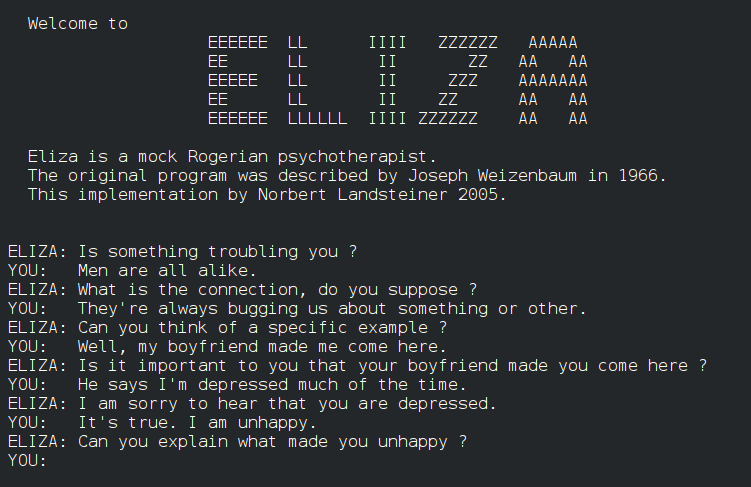
\includegraphics[width=0.75\linewidth]{eliza.png}
        \caption[ELIZA]{ELIZA, an early program for natural language interaction between humans and computers~\cite{wangELIZAChatGPTBrief2024}.}
        \label{fig:eliza}
    \end{wide}
\end{figure}

Even though Weizenbaum already used the term "artificial intelligence" to describe ELIZA~\cite{weizenbaumELIZAComputerProgram1966}, its nature is very different from the modern \glspl{LLM} we know today. He explains ELIZA as follows: "Input sentences are analyzed on the basis of decomposition rules which are triggered by key words appearing in the input text. Responses are generated by reassembly rules associated with selected decomposition rules."~\cite{weizenbaumELIZAComputerProgram1966}. Furthermore, "Keywords and their associated transformation rules constitute the SCRIPT for a particular class of conversation."~\cite{weizenbaumELIZAComputerProgram1966}. These scripts defined both the language (e.g. German or English) and the topic of the conversation via the role ELIZA takes~\cite{weizenbaumELIZAComputerProgram1966}. Weizenbaum found the only "serious" script to be one where ELIZA acts as a psychotherapist~\cite{weizenbaumELIZAComputerProgram1966}, which is the one depicted in \cref{fig:eliza}.

ELIZA works deterministically, as opposed to the probabilistic nature of today's \glspl{LLM}. However, ELIZA shares some abilities with modern \glspl{LLM}: A "rank" was assigned to keywords, so relevant words could be distinguished from less relevant ones~\cite{weizenbaumELIZAComputerProgram1966}. Furthermore, ELIZA was able to understand minimal, specific context via a corresponding script~\cite{weizenbaumELIZAComputerProgram1966}. This is likely why in hindsight, ELIZA is often considered the world's first chatbot~\cite{berryLimitsComputationJoseph2023,shragerELIZAReinterpretedWorlds2024,wangELIZAChatGPTBrief2024}.

Early work in \gls{AI} was mostly theoretical, as both computing power and training data were very limited~\cite{shragerELIZAReinterpretedWorlds2024}. When the internet became prevalent around the year 2000, researchers started compiling internet-scale training datasets~\cite{bankoScalingVeryVery2001,resnikWebParallelCorpus2003,kilgarriffIntroductionSpecialIssue2003}. For the first time, a rich variety of content was available in any language, easily accessible from anywhere in the world. This accelerated the progress in \gls{AI}, and more specifically in \gls{NLP}: In 2011, Apple launched Siri, the first natural language assistant to attract lasting public attention~\cite{wangELIZAChatGPTBrief2024}.

In 2017, the introduction of the Transformer architecture for \glspl{LLM} laid the foundation for the popular chatbots we know today~\cite{vaswaniAttentionAllYou2023}. In turn based on the attention mechanism introduced in 2014~\cite{bahdanauNeuralMachineTranslation2016}, it enabled \glspl{LLM} to consider the context a word is in, instead of processing each word in isolation~\cite{vaswaniAttentionAllYou2023,bahdanauNeuralMachineTranslation2016}. Furthermore, each word is weighted with an attention score, allowing the \gls{LLM} to focus on relevant words~\cite{vaswaniAttentionAllYou2023,bahdanauNeuralMachineTranslation2016} - just like ELIZA, but in a vastly different order of magnitude.

In 2019, after initially deeming too dangerous to make public, OpenAI released GPT-2~\cite{hernNewAIFake2019}. With the release of ChatGPT in December 2022, chatbots finally gained widespread popularity in personal, educational and professional use~\cite{wuUnveilingSecurityPrivacy2024}. \gls{AI} assists researchers and engineers~\cite{schmidgallAgentLaboratoryUsing2025} in anything from solving physics equations~\cite{panQuantumManybodyPhysics2025,songLLMFeynmanLeveragingLarge2025} to writing and debugging code~\cite{shiCodeCorrectnessClosing2024,tianDebugBenchEvaluatingDebugging2024,leeUnifiedDebuggingApproach2024,leeGitHubRecentBugs2024}. In education, they can support individualized learning and automate administrative tasks~\cite{mienyeChatGPTEducationReview2025}. In industries like healthcare and e-commerce, chatbots are used in customer service as they provide instant responses and personalized experiences~\cite{wangELIZAChatGPTBrief2024}. As virtually all industries are influenced in one way or another and user acceptance is high~\cite{wangHistoryDevelopmentPrinciples2024,wangELIZAChatGPTBrief2024}, \gls{AI} is here to stay.

\subsection{Making a virtue out of necessity}
\label{sec:makingAVirtueOutOfNecessity}
While there is much more to discuss about the inner workings of \glspl{LLM} and how they relate to other methods in the field \gls{NLP}, this is not the core of this thesis. Instead, we focus on problems that come with the common usage of \glspl{LLM} in the form of commercial chatbots. This will show us requirements needed for our implementation of text-based steganography to protect user privacy.

With the vast public attention \gls{AI} has gotten in recent years, its commercialization is in full swing~\cite{soniOpenAIOutlinesNew2025}. As \gls{AI} influences increasingly many aspects of our daily lives, it accesses highly sensitive data. For example, it can be used to analyze social media activity~\cite{sufiSocialMediaAnalytics2023}, evaluate health records~\cite{lovonEvaluatingLLMAbilities2025} or support children in school~\cite{mienyeChatGPTEducationReview2025}. As many \gls{AI} applications need significant computing resources, many individuals and organizations are dependent on cloud-based service providers. These service providers may have interest in harvesting our personal data for additional commercial gain~\cite{biddleFacebookEngineersWe2022,mccallumMetaFacebookOwner2023}. Therefore, privacy and security play a central role for long-term viability of \gls{AI}~\cite{guptaChatGPTThreatGPTImpact2023,wuUnveilingSecurityPrivacy2024}.

Commercial chatbots expose many ethical and privacy concerns~\cite{rayBenchmarkingEthicalAlignment2023}. Ethical concerns are centered around pirated training data~\cite{brittainMetaKnewIt2025,vandersarMetaTorrented812025,liesenfeldOpeningChatGPTTracking2023} and working conditions~\cite{perrigoExclusive$2Hour2023}. Privacy issues don't only concern training data, but reach all the way to the end user experience: Malicious users could extract inputs from other users that the \gls{LLM} was trained on, e.g. by jailbreaking via prompt injection or reverse psychology~\cite{guptaChatGPTThreatGPTImpact2023,wuUnveilingSecurityPrivacy2024}. Furthermore, for many users these service providers would not be in their jurisdiction. Foreign law enforcement could therefore demand and obtain access to user data without users being aware of it or having any legal recourse.

We can't solve all of these issues, but we can leverage \glspl{LLM} to combat some of them. We can deduct some requirements for our implementation of text-based steganography from the issues described above:
\begin{itemize}
    \item Our implementation should run the \gls{LLM} locally. This is to ensure data sovereignty by avoiding any chance of leaks from exposing data to a third party.
    \item Our implementation should provide an acceptable performance on today's entry-level smartphones. This is important since running \glspl{LLM} is resource-intensive and we target a very diverse user spectrum.
    \item Our implementation should work offline. This means, once the \gls{LLM} is downloaded, no internet connection should be required. This is within the scope of this thesis, as no server backend for sending messages will be implemented.
    \item Preferably, the \gls{LLM} (and any dependencies) should be open source. This may be achieved by making the \gls{LLM} swappable.
\end{itemize}

Especially the last requirement is more sophisticated than one might think. Many \glspl{LLM} are not open source as per \gls{OSI} definition~\cite{tarkowskiDataGovernanceOpen2025,osiOpenSourceAI,gnuprojectWhatFreeSoftware}. This might be due to training datasets or parameter weights not being available, e.g. in the cases of Llama~\cite{metaMetallamaLlamamodels2025,touvronLLaMAOpenEfficient2023} and DeepSeek~\cite{deepseekDeepseekaiDeepSeekR12025,deepseek-aiDeepSeekR1IncentivizingReasoning2025}, or due to incompatible licenses making them source-available~\cite{liesenfeldOpeningChatGPTTracking2023,whiteModelOpennessFramework2024}.

Training datasets not being disclosed limits our ability to make an educated choice considerably. As an increasing amount of data on the internet is generated by \gls{AI}, it makes its way into future training datasets. This can have a poisoning effect on output quality~\cite{alemohammadSelfConsumingGenerativeModels2023,shumailovCurseRecursionTraining2024,martinezUnderstandingInterplayGenerative2023,martinezCombiningGenerativeArtificial2023}.

Alternatively, we could train our own \gls{LLM}. This would unlock promising perspectives on improving cover text quality. For example, we could personalize the \gls{LLM} by fine-tuning it with past text messages of our own~\cite{donnerSimulationMeFinetuning2024,donnerStepStepGuide2024,donnerFinetuningLLMYour2024,donnerFinetuningLLMYour2024a,donnerFinetuningLLMYour2024b}. However this is not only complex~\cite{huLoRALowRankAdaptation2021} and computationally expensive, but also not necessarily privacy-respecting. On one hand, we may avoid leaks through service providers. On the other hand, we would have to get consent from all people whose chat messages are in our training dataset. For example, for an average Computer Science student at TU Darmstadt taking part in a group chat for every lecture, this could mean over a thousand people.

% !TeX root = ../Thesis.tex

%*****************************************
\chapter{Related Work}\label{ch:relatedwork}
%*****************************************
\glsresetall % Resets all acronyms to not used

Steganography is often described as both the art and science of hiding information~\cite{bennettLinguisticSteganographySurvey2004}. As its forms are only limited by our creativity, an exhaustive discussion is not possible. Instead, we focus on some selected works. By progressing from simple to more sophisticated approaches, we ultimately answer the question: Why use \glspl{LLM} at all?

\section{Steganography without large language models}
\label{sec:steganographyWithoutLLMs}
As we implement an Android app to perform steganography in chat messages locally on smartphones, hardware resources are our strongest limitation. While \glspl{LLM} are a popular option to perform this kind of steganography~\cite{zieglerNeuralLinguisticSteganography2019}, running them is very resource-intensive. Therefore, we first consider some approaches without \glspl{LLM}.

\subsection{Mimicking}
\label{sec:mimicking}
Spammimic is a demonstration of text-based steganography without \glspl{LLM} from as early as 2001~\cite{spammimicSpammimic2000}. Secret messages are encoded into cover texts that look like spam e-mails. \cref{fig:spammimicSpamEmail} shows an example. This is done using context-free grammars and mimic functions~\cite{waynerMimicFunctions1992,bennettLinguisticSteganographySurvey2004}.

\begin{figure}
    \begin{wide}
        \centering
        \captionsetup{width=\linewidth}
        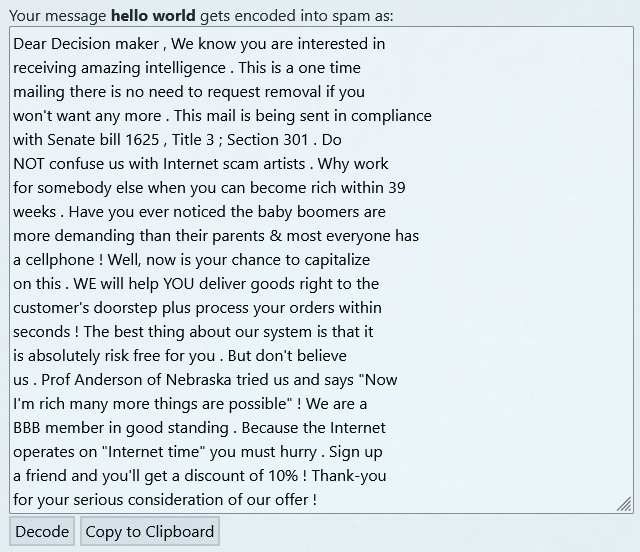
\includegraphics[width=0.5\linewidth]{spammimic_spam_email.png}
        \caption[Spammimic]{Steganography in spam e-mails with Spammimic~\cite{spammimicSpammimic2000}. Only the secret message "hello world" was user input.}
        \label{fig:spammimicSpamEmail}
    \end{wide}
\end{figure}

This approach already fulfills some of the requirements we set ourselves in \cref{ch:introduction}. It generates plausible cover texts for a given topic with minimal computing resources. The topic can be chosen by exchanging the grammar~\cite{spammimicSpammimic2000}. Generating spam e-mails is particularly beneficial as it lowers an attacker's expectation of cover text quality. It allows us to hide our communication amongst other e-mail traffic, obfuscating when a secret communication is happening. We may even send our cover texts to any number of recipients that includes the intended one, to obfuscate who is communicating with whom. Both would increase an attacker's costs significantly~\cite{bennettLinguisticSteganographySurvey2004,petitcolasInformationHidingSurvey1999}.

But there are several drawbacks. Users would have to handle different grammars for different chat conversations. Creating grammars requires expert knowledge. This can't be expected from the average user. In contrast, \glspl{LLM} can be influenced by natural language commands. This can be expected from any layman user. Furthermore, encoding efficiency is low. Any secret message longer than a few words generates cover texts of implausible length, even for a spam e-mail.

\subsection{Substitution}
\label{sec:substitution}
When \gls{SMS} was prevalent, its character limits led users to abbreviate common terms (e.g. "u" for "you"). As shown in ~\cite{shirali-shahrezaTextSteganographySMS2007}, this can be leveraged to perform steganography. We define a dictionary of terms and their abbreviations and let the user write a chat message without any abbreviations. By either substituting terms with their abbreviations or not, we encode 1s and 0s.

This approach again fulfills some of the requirements we set ourselves in \cref{ch:introduction}. It uses minimal computing resources and gives the user great control over cover text quality. Semantically meaningful conversations are guaranteed as terms and their abbreviations are synonymous. A customizable dictionary is already built into the keyboards of most smartphones, so it is easily accessible for the average user.

But there still are several drawbacks. As many terms don't have an abbreviation in practice, encoding efficiency is low. This is aggravated when abbreviations are used for entire sentences instead of individual words (e.g. "ily" instead of "i luv u" for "i love you"). Abbreviations can be undesired for readability or even inappropriate in formal communication. Other substitution approaches (e.g. substituting synonym words) solve these issues only partially.

\section{Steganography with large language models}
\label{sec:steganographyWithLLMs}
While steganography approaches without \glspl{LLM} are already able to fulfill some of the requirements we set ourselves in \cref{ch:introduction}, they all suffer from low encoding efficiency. Therefore, we now consider steganography approaches with \glspl{LLM}. First, we restrict ourselves to high-level access via prompting. Then we investigate a low-level solution by manipulating token generation. This finally leads us to the Stegasuras project~\cite{zieglerNeuralLinguisticSteganography2019}, which this thesis is based on.

\subsection{High-level: Prompting}
\label{sec:highLevelPrompting}
With state-of-the-art \glspl{LLM} reaching hundreds of billions of parameters, they are able to perform advanced logic only by being prompted~\cite{hossainLLMProSAnalyzingLarge2025}. As demonstrated in~\cite{steinebachNaturalLanguageSteganography2024} with ChatGPT, we can leverage this to perform steganography. We define two disjoint sets of words, A and B. We prompt the \gls{LLM} to generate a text that contains words from A and B matching a certain pattern (e.g. BABBABABA). We interpret any occurrence of a word from A as 0, any from B as 1.

This approach is attractive because it doesn't require a low-level understanding of \glspl{LLM} to implement it. The topic of cover texts can be controlled via the words in sets A and B, which in turn can be generated via a prompt. Encoding efficiency can be controlled via the number of word sets to choose from. It may also be relatively efficient with computing resources, as the \gls{LLM} is only needed for encoding, not for decoding.

However, this approach conflicts with most of the requirements we set ourselves in \cref{ch:introduction}. As can quickly be tested with tools like LM Studio, small \glspl{LLM} that are feasible to run locally on a smartphone are not able to perform the encoding logic. We would have to rely on a service provider to host a large \gls{LLM} for us. Making core functionality of our app dependent on third parties increases attack surface significantly (see \cref{sec:largeLanguageModels}). Therefore, the simplicity of this approach is not worth it for us.

\subsection{Low-level: Manipulating token generation}
\label{sec:lowLevelManipulatingTokenGeneration}
Many modern frameworks exist to give us low-level access to \glspl{LLM}. As demonstrated in the Stegasuras project with PyTorch and GPT-2~\cite{zieglerNeuralLinguisticSteganography2019,zieglerHarvardnlpNeuralSteganography2025,zieglerStegasuras2025}, this can be leveraged to perform steganography. First, we convert a secret message from string to binary. Then, we encode it into a cover text by letting the \gls{LLM} sample tokens to complete a given context based on the secret message bits. \cref{fig:stegasuras} shows an example. Stegasuras implements UTF-8 conversion and Arithmetic compression for the first step and Arithmetic, Huffman and Bins coding for the second step.

\begin{figure}
	\begin{wide}
		\captionsetup{width=\linewidth}

		\begin{subfigure}{\linewidth}
			\centering
			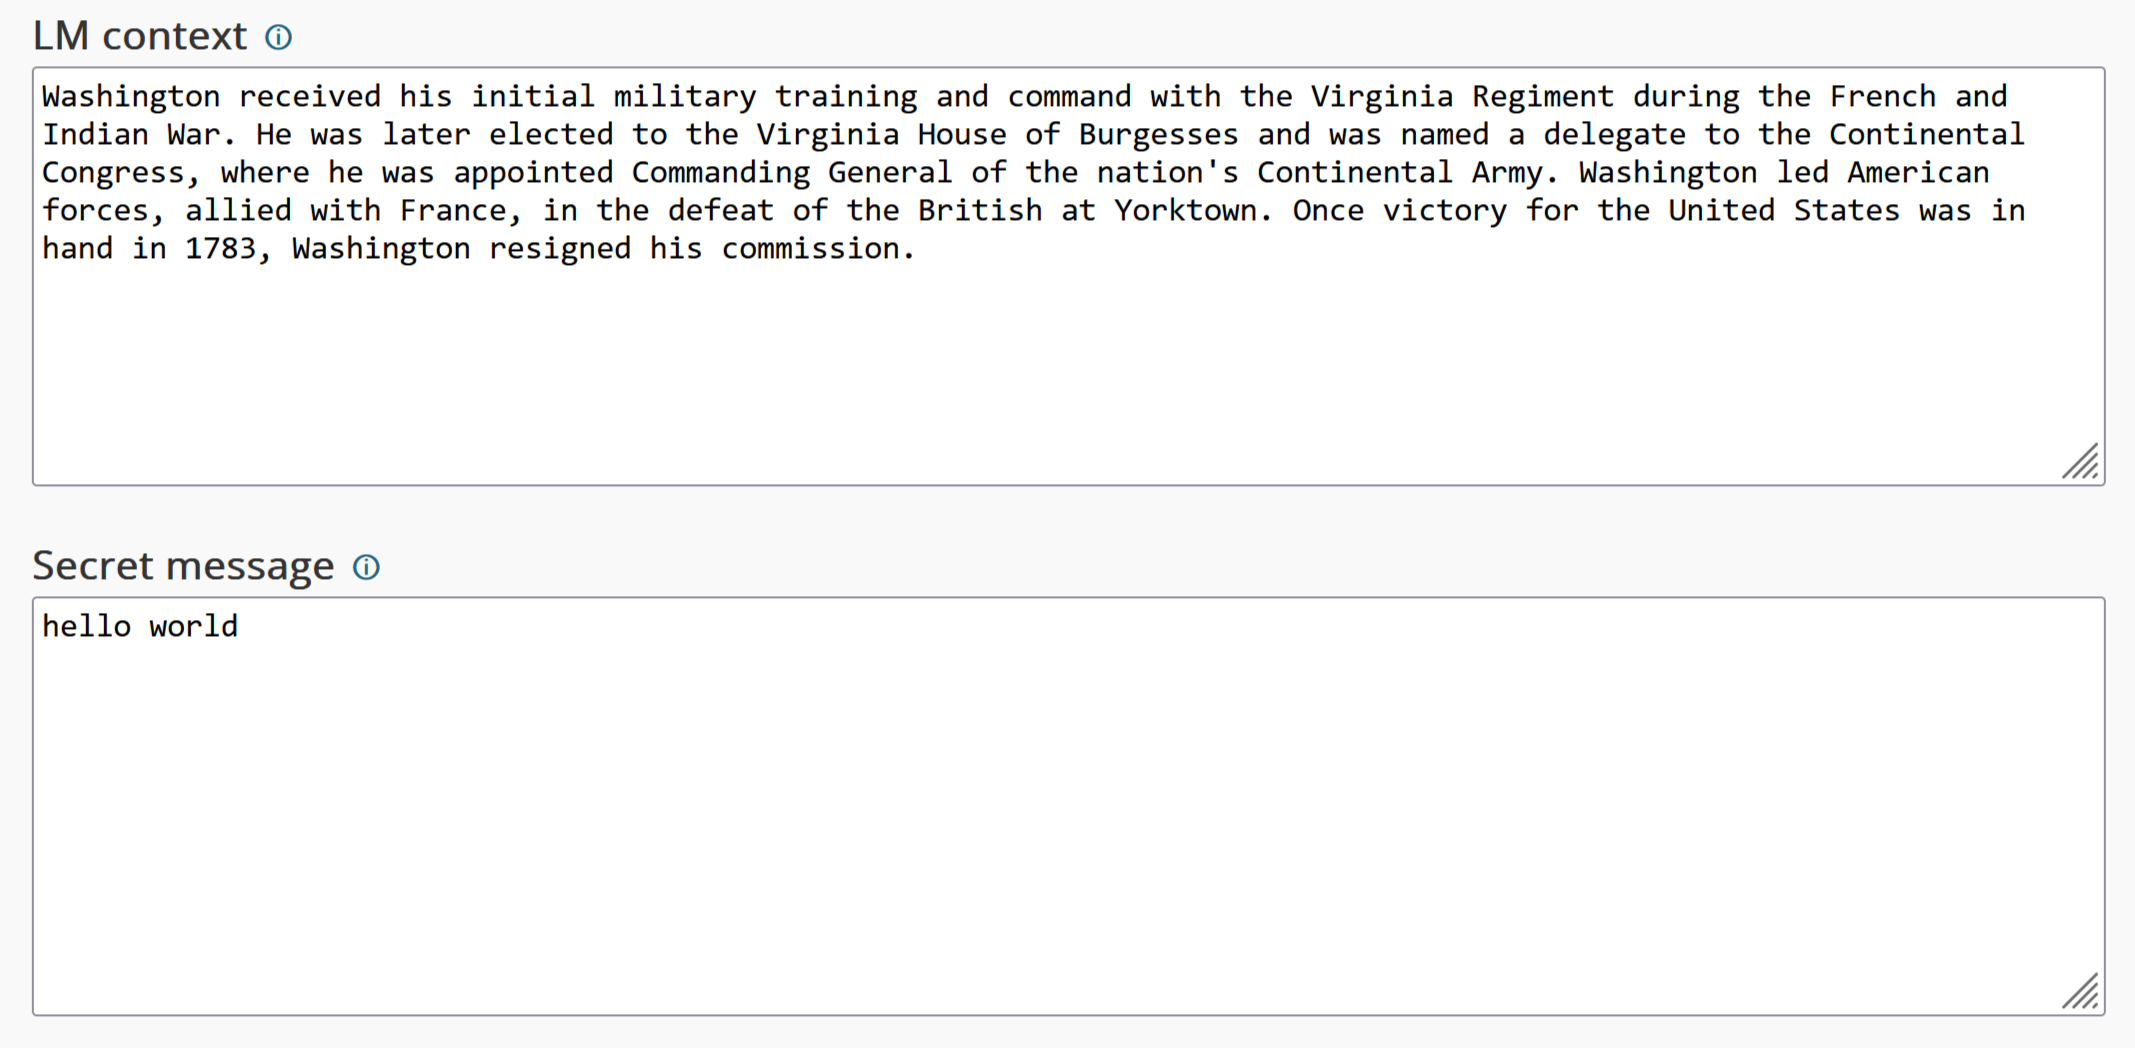
\includegraphics[width=0.75\linewidth]{stegasuras_a.png}
			\caption{Inputs: A context to be completed and the secret message to be encoded.}
			\label{fig:stegasurasA}
		\end{subfigure}

		\begin{subfigure}{\linewidth}
			\centering
			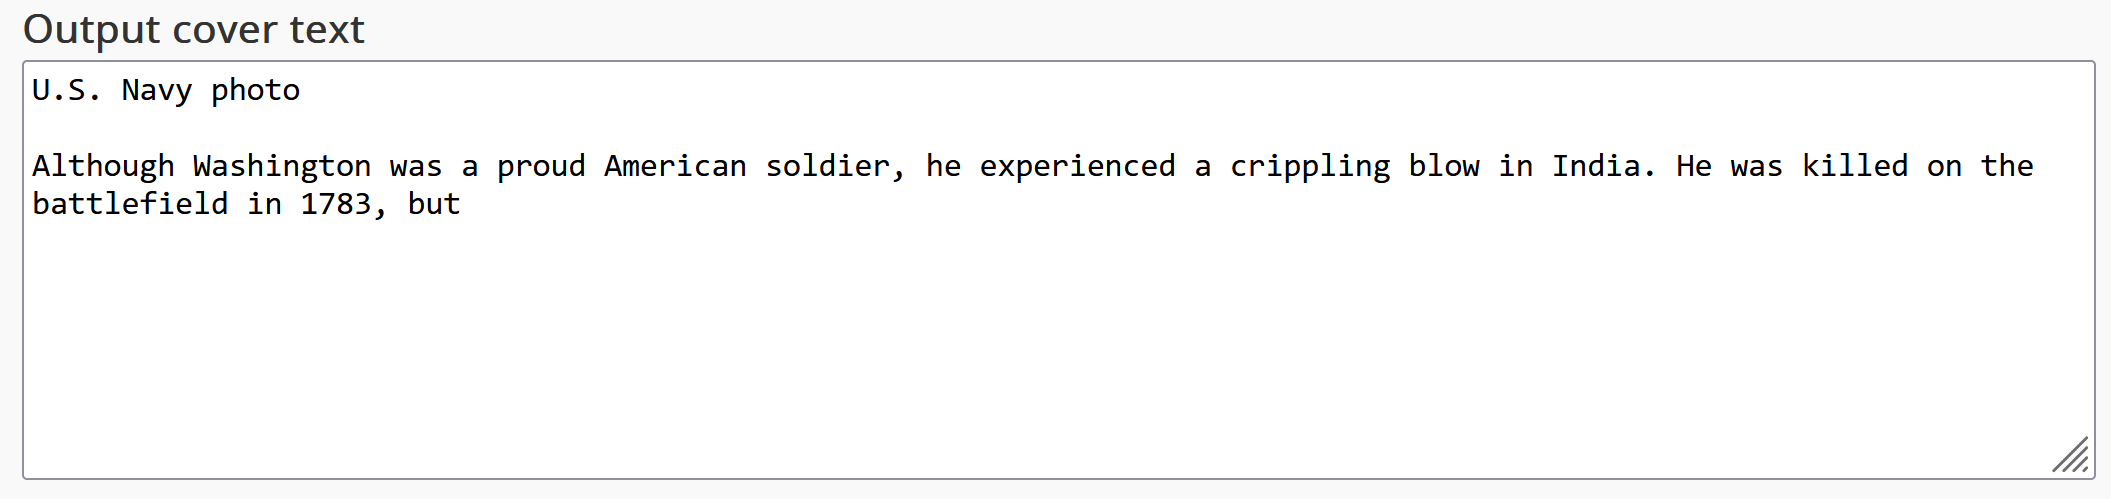
\includegraphics[width=0.75\linewidth]{stegasuras_b.png}
			\caption{Output: A cover text that completes the context while encoding the secret message.}
			\label{fig:stegasurasB}
		\end{subfigure}

		\caption[Stegasuras]{The web demo of Stegasuras~\cite{zieglerStegasuras2025}.}
		\label{fig:stegasuras}
	\end{wide}
\end{figure}

This approach is promising several strengths we haven't seen before. By gaining low-level access to the \gls{LLM}, we can implement a complex encoding logic. This increases encoding efficiency to multiple bits per token and allows us to use small \glspl{LLM} that are feasible to run locally on a smartphone.

However, the Stegasuras implementation also has some shortcomings we can improve upon. Being published in 2019, it is not state-of-the-art anymore. We can expect significant gains in cover text quality by just swapping out the \gls{LLM}~\cite{wuGenerativeTextSteganography2024}. Furthermore, there is an open edge case. Cover text generation ends as soon as all secret message bits are encoded, so the last sentence doesn't get finished~\cite{zieglerStegasuras2025}. Stegasuras offers a partial solution by finishing it with greedy sampling during encoding~\cite{zieglerHarvardnlpNeuralSteganography2025}, but this isn't considered during decoding and therefore adds noise. Stegasuras ignores this in its evaluation by cutting off unfinished last sentences~\cite{zieglerNeuralLinguisticSteganography2019}, thereby corrupting the secret message encoded in them.

Solving this edge case is the first contribution we make. Beyond that, we port the implementation to the state-of-the-art llama.cpp framework~\cite{gerganovGgerganovLlamacpp2024}, which gives us access to a wide range of \glspl{LLM} to scale with available hardware. We implement an Android app to run all of this locally on a smartphone. We extend the functionality by creating chat conversations, allowing users to arbitrarily interleave cover texts and plain texts. We improve cover text quality by including emojis and exposing a system prompt, allowing users to influence \gls{LLM} behaviour on a lower level via a natural language command. This way, we are able to solve the real-world problem of protecting people's privacy against eavesdroppers with steganography.

% \section{Further considerations}
% \label{sec:furtherConsiderations}
% In the previous sections of this chapter, we discussed several approaches for text-based steganography without \glspl{LLM}. In particular, we focussed on the extent to which each approach fulfilled our central requirement - creating a believable chat conversation from cover texts. In this section, we take a look at some more text-based steganography approaches, still without involving \glspl{LLM}. But the focus is now on some more refined requirements, stemming from more specific use cases. Lastly, we take a look at an example of what not to do.

% \subsection{Localization}
% \label{sec:localization}
% The overall goal of our implementation can be stated as follows: Use text-based steganography in chat messages to protect against attackers. While multiple aspects of this definition can and will be refined over the course of this thesis, we now discuss one aspect that is largely omitted otherwise: Localization. Our standard assumption is that both users and attackers are English-speaking. This may be fine for academic purposes, but in practice a lot of the potential users of our implementation are in countries where English is not an official language. This is especially relevant for protection from political persecution under authoritarian regimes.

% An example implementation of location-specific steganography is Nahoft~\cite{united4iranNahoft2021,united4iranU4iadminNahoft2025}. This is an Android app designed to protect people in Iran protesting against their government. It performs text-based steganography by creating cover texts consisting of random Persian words, the official language of Iran. If English was used in this situation, it would only attract unwanted attention from the authorities.

% Characteristics specific to languages with non-Latin scripts can be leveraged for steganography. Examples for such languages are Arabic~\cite{shirali-shahrezaNewApproachPersian2006,hamzahLinguisticSteganographyFramework2021,thabitComparativeAnalysisArabic2021}, Chinese~\cite{luoTextSteganographyHigh2017} and Hindi~\cite{allaEvolutionHindiText2009}. The scripts of these languages provide a rich variety of symbols and variations, exceeding what the Latin script has to offer, allowing e.g. multiple equivalent shapes for the same expression~\cite{shirali-shahrezaNewApproachPersian2006,hamzahLinguisticSteganographyFramework2021,thabitComparativeAnalysisArabic2021}. Furthermore, relationships between languages should be considered. Steganography approaches leveraging language-specific characteristics can sometimes be transferred to related languages~\cite{allaEvolutionHindiText2009}.

% The challenge of localization can partially be solved with our implementation. As~\cref{ch:design} will explain in detail, one goal of our implementation is that the \gls{LLM} can be swapped out easily. While this doesn't enable us to leverage language specifics like changing character shapes, it enables us to choose a \gls{LLM} that was trained on any natural language desired. If we are able to generate semantically meaningful cover texts in any language, further localization might not be necessary. We could use our implementation in any geo-political conflict, deliberately speaking (or not speaking) the language of the attacker. But verifying this is unfortunately out of scope for this thesis, as the author doesn't speak any languages with non-Latin scripts.

% \subsection{A negative example}
% \label{sec:aNegativeExample}
% Lastly, we take a look at an example of what not to do, so we can avoid it in our implementation. We recall that steganography violates Kerckhoffs' principle~\cite{andersonLimitsSteganography1998}, as the security of a steganographic system partially relies on the attacker not knowing the system - or that it is being used in the first place.

% An approach for text-based steganography in e-mails is shown in~\cite{malikHighCapacityText2017}. Similar to our implementation, it uses Huffman compression to convert a secret message from string to binary. But instead of generating a cover text with \glspl{LLM}, an edit-based approach is chosen by taking the cover text from user input. Information is encoded by colour coding the cover text, with colours being selected from a user-defined colour table. \cref{fig:colourCoding} shows the example given in~\cite{malikHighCapacityText2017}. As~\cite{malikHighCapacityText2017} proposes, this approach is suitable for personal messages containing congratulations, poems, etc. Users may try to obfuscate the steganography as they have full control over cover text quality and the colour table, e.g. by choosing black, dark grey, light grey and white as colours.

% \begin{figure}
%     \begin{wide}
%         \centering
%         \captionsetup{width=\linewidth}
%         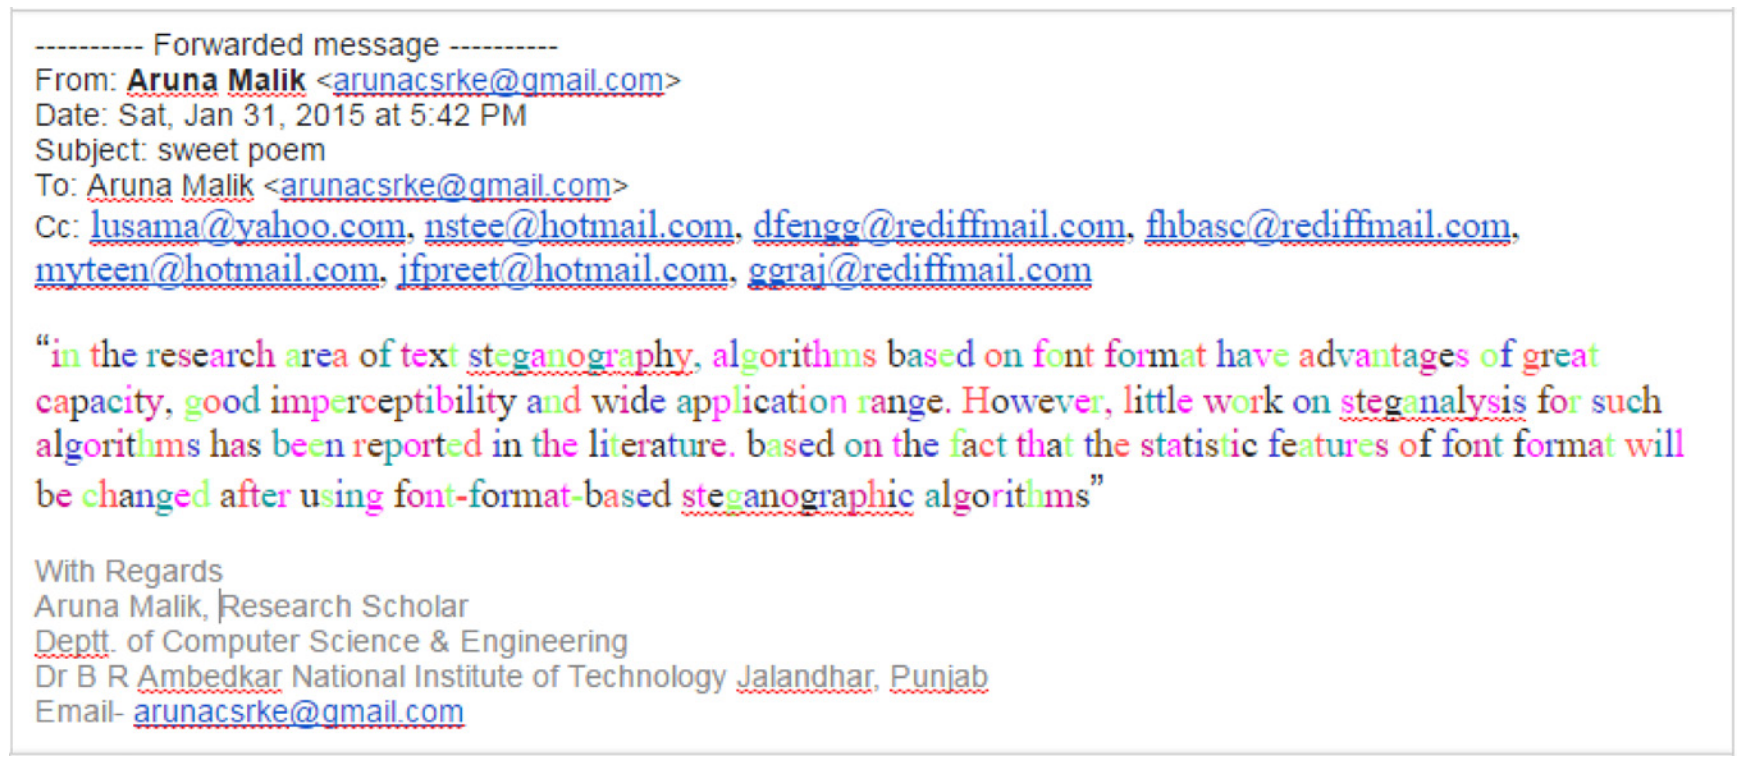
\includegraphics[width=0.75\linewidth]{colour_coding.png}
%         \caption[Colour coding]{Steganography via colour coding~\cite{malikHighCapacityText2017}.}
%         \label{fig:colourCoding}
%     \end{wide}
% \end{figure}

% However, this doesn't outweigh the disadvantages. The colour table has to be exchanged between sender and receiver, which is difficult as it is not natural language. This approach also is not robust when using non-digital communication channels, as the colour coding is lost if the cover text is spoken during a phone call or printed out in black and white. The proposed use case is very narrow, as an attacker should become suspicious if this is used in any other setting. More generally, the colour coding introduces an unnatural communication pattern that might make it obvious to an attacker that a secret communication is happening. This breaks the additional layer of security that is supposed to be introduced by steganography. We can transfer this to our implementation by avoiding e.g. uncommon use of abbreviations or emojis in the generated chat conversations. Furthermore, we should also avoid introducing unnatural restrictions, e.g. assuming that chat messages are being sent with strictly alternating roles of sender and receiver. \cref{ch:implementation} will show that this is only partially possible in our implementation.

\iftoggle{parts}{
	\cleardoublepage
	\ctparttext{The contribution starts with a design chapter, where we mathematically describe the design of the physical layer security system, as well as the adaptive filter of the attacker. After the design follows the implementation on WARP nodes. Here we give an insight into the challenges of implementing the designed MIMO communication system. The last chapter concentrates on evaluating the performance of our proposed attack in simulation and practice.}
	\partExtra{Contribution}
}{}
% !TeX root = ../Thesis.tex

%************************************************
\chapter{Design}\label{ch:design}
%************************************************
\glsresetall % Resets all acronyms to not used

To implement steganography with local \glspl{LLM} on Android, we have to make some important design decisions. This encompasses the choice of \gls{LLM} and the framework to run it. To support these decisions, we revisit the Stegasuras project, which our app is based on.

\section{Overview of requirements and architecture}
\label{sec:overviewOfRequirementsAndArchitecture}
Our work is based on the Stegasuras project~\cite{zieglerNeuralLinguisticSteganography2019}, which demonstrates how to perform steganography by manipulating token generation of a \gls{LLM}. Fundamentally, it works as follows: First, we convert a secret message from string to binary. Then, we encode it into a cover text by letting the \gls{LLM} sample tokens to complete a given context based on the secret message bits. Stegasuras has a modular architecture, as it implements multiple algorithms for each of the two steps. This approach is promising for fulfilling the requirements we set ourselves in \cref{ch:introduction}:
\begin{enumerate}
    \item Create a chat conversation between cover texts by generating them with a \gls{LLM}.
    \item Run the \gls{LLM} locally on an Android smartphone, i.e. don't require any internet connection for the steganography itself.
    \item Achieve acceptable performance on entry-level devices.
    \item Make the \gls{LLM} swappable.
\end{enumerate}

But as Stegasuras uses GPT-2 as \gls{LLM}, it is not state-of-the-art anymore. Furthermore, it uses the PyTorch framework to run the \gls{LLM}. As a Python library, PyTorch can't natively be run on Android. Therefore, we investigate modern \glspl{LLM} and the frameworks to run them in \cref{sec:howToRunLLMsOnAndroid,sec:howToSelectASuitableLLM}. This results in the following architecture:
\begin{itemize}
	\item Our app is mainly written in Kotlin, with Jetpack Compose as a \gls{UI} framework. This is to ensure easy maintainability.
	\item We integrate some C++ code to run the \gls{LLM} using the llama.cpp library~\cite{gerganovGgerganovLlamacpp2024}. This gives us access to a wide range of \glspl{LLM} readily available in the \lstinline|.gguf| file format.
	\item We use Llama 3.2 1B~\cite{huggingquantsHuggingquantsLlama321BInstructQ4_K_MGGUFHugging2024} as \gls{LLM} for our evaluation. This is because it is able to hold a conversation while being small enough to run on entry-level smartphones.
\end{itemize}

Beyond that, we only rely on native Androidx and Kotlinx libraries to introduce as little third party dependencies as possible.

\section{How to run large language models on Android}
\label{sec:howToRunLLMsOnAndroid}
To implement steganography as demonstrated by Stegasuras~\cite{zieglerNeuralLinguisticSteganography2019} on Android, we have to find a \gls{LLM} runtime that supports the \gls{JVM}~\cite{ruggiaDarkSideNative2025}. This restricts our choice of programming languages to Java and Kotlin~\cite{ruggiaDarkSideNative2025}, which conflicts with the Python library PyTorch used by Stegasuras. By including C++ code via the \gls{JNI}~\cite{ruggiaDarkSideNative2025}, we find llama.cpp as a solution~\cite{gerganovGgerganovLlamacpp2024}.

\subsection{PyTorch}
\label{sec:pyTorch}
Our implementation of steganography in chat messages using local \glspl{LLM} on Android is based on the Stegasuras project~\cite{zieglerNeuralLinguisticSteganography2019}. As Stegasuras is written in Python, it uses the PyTorch~\cite{anselPyTorch2Faster2024} and HuggingFace Transformers~\cite{wolfTransformersStateoftheArtNatural2020} libraries to run the \gls{LLM} locally. Originally developed by Facebook (now Meta) since 2016, PyTorch is now part of the Linux Foundation~\cite{chintalaPyTorchStrengthensIts2022}. It also comes with its own tensor library called ATen~\cite{devitoZdevitoATen2025}.

Finding a way to run PyTorch on Android was the obvious first approach. Unfortunately, Python support on Android is not officially endorsed by Google. Some language bindings to Kotlin or Java exist for PyTorch, but none of them are actively maintained. Alternatively, we could use libraries for building cross-platform Python applications~\cite{kivyKivyKivy2025}, but they share a common concern. As Python integration requires another abstraction layer, this could introduce a significant performance overhead. This could conflict with one of the requirements we set ourselves in \cref{ch:introduction}: Acceptable performance on entry-level smartphones. Ultimately, no option was attractive enough to commit to it.

Furthermore, the industry is centered around Kotlin as the language officially endorsed by Google~\cite{ruggiaDarkSideNative2025}. Java as its predecessor is being phased out, but its libraries remain interoperable. C++ may be preferred for performance, but its manual memory management may also make our app more prone to security vulnerabilities~\cite{ruggiaDarkSideNative2025}. The PyTorch ecosystem offers multiple distributions that could help us here~\cite{pytorchPyTorch}:
\begin{itemize}
	\item PyTorch, the original Python library~\cite{anselPyTorch2Faster2024}.
	\item PyTorch Mobile, for Android and iOS~\cite{pytorchPytorchAndroiddemoapp2025}.
	\item ExecuTorch, for Android and iOS~\cite{pytorchPytorchExecutorch2025}.
	\item libtorch, the Java and C++ distributions of PyTorch~\cite{pytorchStartLocally,pytorchPyTorchAPIPyTorch}.
\end{itemize}

Upon closer inspection, none of them seemed production-ready for Android. PyTorch Mobile is no longer maintained~\cite{pytorchPytorchAndroiddemoapp2025}, while ExecuTorch is still in its beta phase~\cite{pytorchPytorchExecutorch2025}. Documentation about libtorch was conflicting, as it is claimed to be stable in some places and marked unstable in others~\cite{pytorchStartLocally,pytorchPyTorchAPIPyTorch}. Furthermore, there was a lack of both open source projects using PyTorch on Android and \glspl{LLM} readily available on platforms like HuggingFace~\cite{huggingfaceModelsHuggingFace2025}. While a lot of base models are available in the PyTorch format, their quantizations are not. Ultimately, PyTorch was ruled out because the expected compromises could not be justified.

\subsection{llama.cpp}
\label{sec:llamaCpp}
As investigating the popular PyTorch ecosystem didn't yield any example projects from the open source community, we changed our research approach. Instead of looking for frameworks and then trying to find examples, we now looked for examples to then find out what frameworks they use. We searched the Google Play Store and GitHub for Android apps that offer a functionality to chat with local \glspl{LLM}. This approach was more successful, as we found three apps that use the same framework: llama.cpp~\cite{panchalShubham0204SmolChatAndroid2025,vali-98Vali98ChatterUI2025,ghorbaniAghorbaniPocketpalai2025}. While these apps are projects by hobbyists, they allowed us to judge llama.cpp by seeing it in action.

We installed the apps onto a Moto One Vision, the Android smartphone we used during most of the development of our app. By today's standards, a Moto One Vision with its 4 GiB of memory is an entry-level device. All three apps allowed the user to run any \gls{LLM} from a \lstinline|.gguf| file. We chose a 4 bit quantization of Llama 3.2 1B (see \cref{sec:howToSelectASuitableLLM} for details). We deemed performance acceptable if the \gls{LLM} was able to generate a response with at least 1 token/second throughout a small conversation of ten messages. All apps performed more than acceptably, generating responses with around 5 tokens/second. Later testing on a flagship Samsung Galaxy S24 Ultra even achieved around 25 tokens/second. These results gave us confidence that we can fulfill our performance requirement with llama.cpp.

With this insight, we investigated llama.cpp further. It became apparent that it offers several benefits over PyTorch. Developed by Georgi Gerganov since 2023, it does not have any third party dependencies~\cite{gerganovGgerganovLlamacpp2024}. A vast selection of \glspl{LLM} on HuggingFace is quantized from their base model using llama.cpp~\cite{huggingfaceModelsHuggingFace2025}. Quantizations are stored as self-contained \lstinline|.gguf| files~\cite{huggingfaceGGUF}. This gave us confidence that can fulfill another requirement: Making the \gls{LLM} swappable. Furthermore, llama.cpp is both very popular by itself (e.g. by GitHub stars) and as a library to be included in other software (e.g. in LM Studio, Ollama)~\cite{gerganovGgerganovLlamacpp2024}. Its GitHub repository contains a number of examples for basic usage and even a demo Android app~\cite{gerganovGgerganovLlamacpp2024}. Lastly, it comes with its own tensor library, ggml~\cite{gerganovGgerganovGgml2024}. This makes a complete software suite for \glspl{LLM}: llama.cpp as runtime, ggml for tensor operations, \lstinline|.gguf| as file format.

% Add some space on top of listing to match bottom
\vspace{0.25cm}

% Put listings above last paragraph to avoid page break
\begin{lstlisting}[caption={[PyTorch]{Snippet of the Stegasuras code needed to get logits from a \gls{LLM} using PyTorch~\cite{zieglerHarvardnlpNeuralSteganography2025}. Tensor operations are exposed whenever indices of an object are queried.}}, label={lst:pyTorch}]
logits, past = model(prev.unsqueeze(0), past=past)

past = limit_past(past)

logits, indices = logits[0, -1, :].sort(descending=True)
\end{lstlisting}

\begin{lstlisting}[caption={[llama.cpp]{Snippet of our code needed to get logits from a \gls{LLM} using llama.cpp. No tensor operations are exposed.}}, label={lst:llamaCpp}]
if (llama_model_has_encoder(model)) { llama_encode(ctx, batch); }

llama_decode(ctx, batch);

float* logits = llama_get_logits(ctx);
\end{lstlisting}

Of course, llama.cpp comes with some downsides too. As it is a C++ library, it will make our app harder to maintain. It is still very young for a project of this complexity, so some breaking changes are to be expected. But seeing it work in practice was good enough of an argument to commit to it. Experience throughout the course of this thesis showed that llama.cpp was a good choice. It offers significantly better abstractions than PyTorch, hiding tensor operations largely away. Our implementation turned out to be easier to understand and work with than the original PyTorch implementation of Stegasuras~\cite{zieglerHarvardnlpNeuralSteganography2025}. For example, Listings~\ref{lst:pyTorch} and~\ref{lst:llamaCpp} show snippets of the code needed to get logits (unnormalized probabilities) from the \gls{LLM} to predict the next token (see \cref{sec:tokenGenerationWithLlamaCpp} for details).

\subsection{Other options}
\label{sec:otherOptions}
Besides the two major frameworks discussed above, we also investigated many others. To eventually consider them in future projects, we present a selection of the most noteworthy ones here:
\begin{itemize}
	\item TensorFlow, developed by Google, is the main competitor to PyTorch~\cite{abadiTensorFlowLargescaleMachine2015}. While its ecosystem is less fragmented~\cite{googleaiedgeteamTensorFlowLiteNow2024}, it shares most other drawbacks. Availability of \glspl{LLM} in the required format was the main problem.
	\item Jax, developed by Google, is being marketed as a possible successor to TensorFlow~\cite{jaxJaxmlJax2025}. As it is still a research project, it is not an official Google product yet. Again, availability of \glspl{LLM} was the main problem.
	\item ONNX Runtime, developed by Microsoft, promises to be a unified runtime for \glspl{LLM} across formats, platforms and programming languages~\cite{onnxruntimedevelopersONNXRuntime2018}. While this means it could support quantized \glspl{LLM} in the \lstinline|.gguf| file format, availability of example projects was an issue again.
	\item llamafile, developed by Mozilla, promises to run \glspl{LLM} from a single file~\cite{mozillaMozillaOchoLlamafile2025}. As it is built on top of llama.cpp, which already does this, there is no clear benefit for us.
\end{itemize}

We considered a number of projects more specific to Java/Kotlin as well, but dropped them mostly due to lack of popularity and active maintenance.

\section{How to select a suitable large language model}
\label{sec:howToSelectASuitableLLM}
With llama.cpp selected as the runtime environment, we have a wide variety of compatible \glspl{LLM} readily available in the \lstinline|.gguf| file format~\cite{huggingfaceModelsHuggingFace2025}. Now we need to investigate which \glspl{LLM} are suitable for our use case.

As we require our implementation to run on entry-level smartphones, hardware is the most limiting factor. More specifically, the amount of usable memory needs to be large enough to hold the \gls{LLM}, plus some overhead for the app process itself. \cref{tab:smartphones} gives an overview of the smartphones we used for testing. The baseline device is a Moto One Vision. Released to market in 2019, it can be considered entry-level by today's standards. According to the developer settings, around 1.5 GiB out of its 4 GiB of memory are available to applications, with the rest being occupied by the Android operating system. This suggests that we should be able to run \glspl{LLM} with a file size of around 1 GiB on it. Since our Moto One Vision is a typical smartphone with stock hardware and software, we expect this limitation to be similar on current entry-level devices.

\begin{table}
	\centering
	\begin{tabular}{@{} lr @{}} % @{} removes white spaces
		\toprule
		\tableheadline{Smartphone} & \tableheadline{Memory} \\
		\midrule
		Moto One Vision          &  4 GiB \\
		Moto E13                 &  8 GiB \\
		Samsung Galaxy S24 Ultra & 12 GiB \\
		\bottomrule
	\end{tabular}
	% Use alternative short title for table of contents
	\caption[Smartphones]{The smartphones we used for performance evaluation.}
	\label{tab:smartphones}
\end{table}

Initially, this was good enough to browse platforms like HuggingFace~\cite{huggingfaceModelsHuggingFace2025} and find some \gls{LLM} that would run on our hardware. But to make an educated decision, we need to understand which specifications of a \gls{LLM} determine its resource usage and output quality. The most detailed information about a \gls{LLM} can be found in its model card, which effectively is the \lstinline|README.md| of its repository~\cite{mitchellModelCardsModel2019,huggingfaceModelCards}. A model card is supposed to describe all relevant aspects of the \gls{LLM}, such as its architecture, fine-tuning, training dataset, natural languages, license, use cases, and limitations~\cite{mitchellModelCardsModel2019,huggingfaceModelCards}. Unfortunately, the information given in model cards often is incomplete or vague. Alternatively, we can consult the file naming convention, which is used a lot more uniformly. Consider this file name of a Llama 3.2 1B quantization~\cite{huggingquantsHuggingquantsLlama321BInstructQ4_K_MGGUFHugging2024}:

\begin{center}
	\lstinline|llama-3.2-1b-instruct-q4_k_m.gguf|
\end{center}

\begin{itemize}
	\item \lstinline|llama-3.2| is the name and generation of the \gls{LLM}~\cite{metaMetallamaLlamamodels2025}.
	\item \lstinline|1b| is the parameter count of the \gls{LLM}, i.e. 1 billion parameters~\cite{huggingfaceGGUF}.
	\item \lstinline|instruct| is the type of fine-tuning the \gls{LLM} underwent, i.e. it was fine-tuned for instruction-following tasks~\cite{huggingfaceGGUF}.
	\item \lstinline|q4_k_m| is the level the \gls{LLM} was quantized to, i.e. 4 bits per parameter, and some settings used in the process~\cite{huggingfaceGGUF}.
\end{itemize}

This highlights some specifications of the \gls{LLM}: parameter count, fine-tuning and quantization. While parameter count and quantization influence both resource usage and general output quality, fine-tuning only influences output quality given a specific use case. Multiple fine-tunings may be suitable for our use case of creating a chat conversation from cover texts. For example, \lstinline|instruct| or \lstinline|chat| are likely to be preferred over \lstinline|coder| or \lstinline|math|. While a \lstinline|chat| fine-tuning may sound like the obvious choice, it is not as popular as the others. As we may get the \gls{LLM} to generate chat messages by \textit{instructing} it to do so, we chose an \lstinline|instruct| fine-tuning instead. However, judging different \gls{LLM} architectures in detail is out of scope for this thesis.

With this knowledge, we created a selection of \glspl{LLM} that can hold a believable conversation. As our implementation on Android wasn't ready yet, we had to resort to running \glspl{LLM} on desktop using LM Studio. This was done on a Lenovo ThinkPad X1 Tablet (3rd gen) with 16 GiB of memory and an Intel i7-8550U processor. As we set ourselves the requirement of creating a chat conversation from cover texts, users of our app should be able to let the \gls{LLM} generate cover texts that reply to other cover texts generated by their chat partners. Effectively, this means the \gls{LLM} talks to itself without knowing it. We simulated this by opening two instances of LM Studio, both loading the same \gls{LLM} into memory. We gave the first instance a prompt that instructed it on how to start a conversation. While we tried multiple different approaches, they all specified the following requirements: The \gls{LLM} has to take on a certain role in a chat conversation. It has to talk about a certain topic that is typical for this role. Its tone has to be suitable for both role and topic, concerning e.g. use of phrases, abbreviations and emojis. The \gls{LLM} should then respond with a chat message fulfilling these requirements. \cref{fig:lmStudioA} shows examples of both prompt and response using Llama 3.2 1B~\cite{huggingquantsHuggingquantsLlama321BInstructQ4_K_MGGUFHugging2024}.

We then gave the second instance a prompt that instructed it on how to respond to the first instance. While we kept the structure of this prompt the same as detailed above, we tried variations in both role and tone. Roles may either be similar (e.g. two friends, two colleagues) or opposite (e.g. parent and child, employee and customer). The same goes for the tone. \cref{fig:lmStudioB} shows examples of both prompt and response for similar role and tone.

\begin{figure}
	\captionsetup{width=\linewidth}

	\begin{subfigure}{\linewidth}
		\centering
		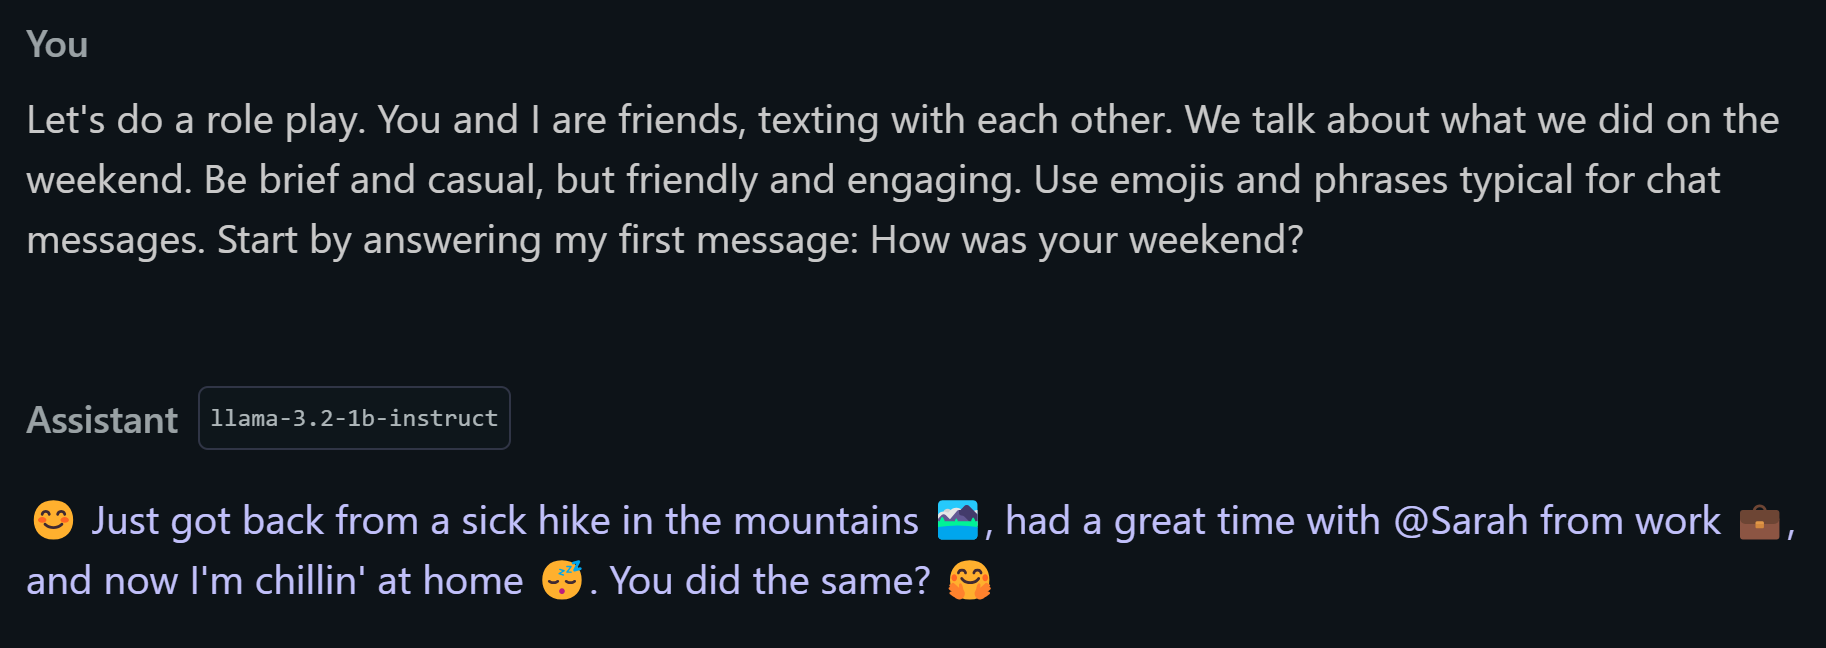
\includegraphics[width=0.75\linewidth]{lm_studio_a.png}
		\caption{The first instance of the \gls{LLM} being instructed on how to start a conversation.}
		\label{fig:lmStudioA}
	\end{subfigure}

	\begin{subfigure}{\linewidth}
		\centering
		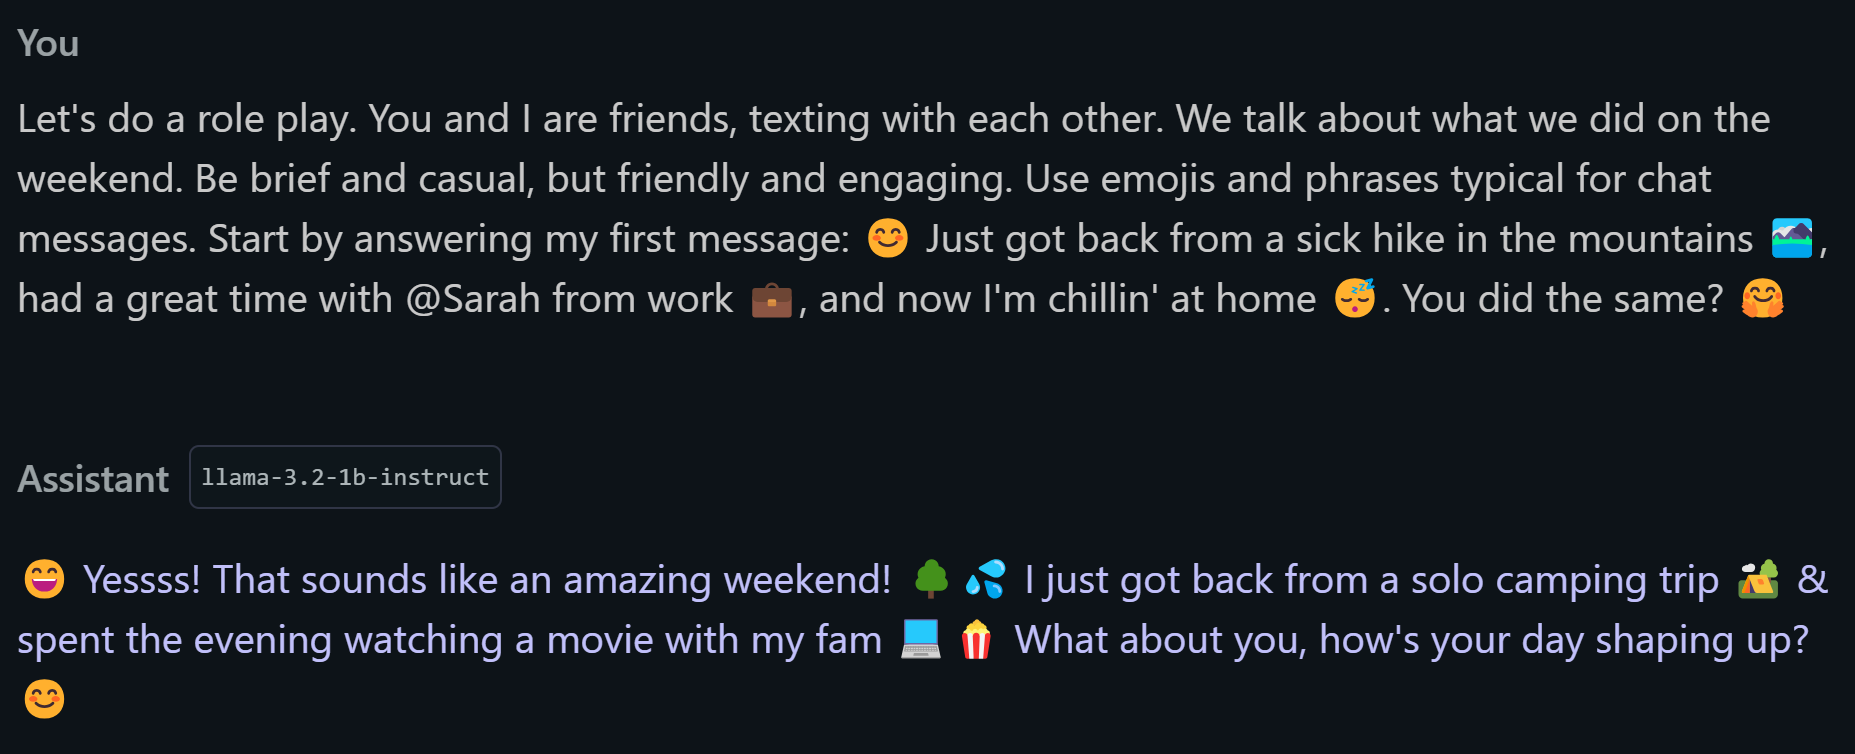
\includegraphics[width=0.75\linewidth]{lm_studio_b.png}
		\caption{The second instance of the \gls{LLM} being instructed on how to respond to the first instance.}
		\label{fig:lmStudioB}
	\end{subfigure}

	\caption[LM Studio]{Use of LM Studio for \gls{LLM} selection.}
	\label{fig:lmStudio}
\end{figure}

From then on, the two instances could talk to each other by copy-pasting their responses back and forth. \cref{tab:largeLanguageModels} shows a selection of popular \glspl{LLM} that we tested using this method. As discussed above, we focus on \glspl{LLM} with around 1 GiB in file size to target entry-level smartphones. On flagship devices, we would choose \glspl{LLM} with higher parameter count or higher number of bits in quantization.

% Windows displays file sizes in MiB, Android in MB
\begin{table}
	\centering
	\begin{tabular}{@{} l p{3cm} p{3cm} r r @{}} % @{} removes white spaces
		\toprule
		\tableheadline{LLM} & \tableheadline{Fine-tuning} & \tableheadline{Quantization} & \tableheadline{File size} & \tableheadline{Source} \\
		\midrule
		Llama 3.2 1B     & Instruct & Q4 &   770 MiB & \cite{huggingquantsHuggingquantsLlama321BInstructQ4_K_MGGUFHugging2024} \\
        Gemma 3 1B       & Instruct & Q4 &   768 MiB & \cite{lmstudiocommunityLmstudiocommunityGemma31bItGGUF2025} \\
		Qwen 2 1.5B      & Instruct & Q4 &   940 MiB & \cite{qwenQwenQwen215BInstructGGUFHugging2024} \\
		SmolLM 2 1.7B    & Instruct & Q4 & 1,007 MiB & \cite{huggingfacesmolmodelsresearchHuggingFaceTBSmolLM217BInstructGGUFHugging2024} \\
        DeepSeek R1 1.5B &      n/a & Q4 & 1,066 MiB & \cite{lmstudiocommunityLmstudiocommunityDeepSeekR1DistillQwen15BGGUFHugging2025} \\
		\bottomrule
	\end{tabular}
	% Use alternative short title for table of contents
	\caption[Large language models]{The \glspl{LLM} we considered. Note that DeepSeek R1 1.5B doesn't specify a fine-tuning.}
	\label{tab:largeLanguageModels}
\end{table}

We prefer Llama 3.2 1B over the other \glspl{LLM} as it was able to create the most believable conversations in our subjective judgement. It tended to give longer answers and consequently hold the conversation for longer. It is able to output emojis, which we can leverage to improve cover text quality. Furthermore, it achieved around 15~tokens/second when generating its response on our desktop system. Gemma 3 1B achieved similar quality and speeds compared to Llama 3.2 1B, but tended to give shorter answers and end the conversation early by itself. Qwen 2 1.5B and SmolLM 2 1.7B achieved similar quality and length compared to Llama 3.2 1B, but only at around half the speeds. Lastly, DeepSeek R1 1.5B was tested. Unlike the other \glspl{LLM}, it exposes a "chain of thought" leading up the the actual response~\cite{deepseek-aiDeepSeekR1IncentivizingReasoning2025}. While this may be beneficial for complex tasks like solving equations, it is not suitable for our use case. It spent around 30 seconds "thinking" before outputting its response. The thought process showed that it often understood our prompts slightly wrong, leading it to drop out of the requested role after a few messages.

% !TeX root = ../Thesis.tex

%************************************************
\chapter{Implementation}\label{ch:implementation}
%************************************************
\glsresetall % Resets all acronyms to not used

\gls{HiPS} is our implementation of steganography in chat messages using local \glspl{LLM} on Android. Based on the Stegasuras project~\cite{zieglerNeuralLinguisticSteganography2019}, this involves two fundamental steps. First, we convert a secret message from string to binary and compress it in the process. Then we encode it into a cover text by letting a \gls{LLM} sample tokens to complete a given context based on the secret message bits.

We discuss the details of our app as follows: First, we give a high-level overview in \cref{sec:overviewOfTheApp}. Then we show how Java/Kotlin and C++ code can interact using the \gls{JNI} in \cref{sec:javaNativeInterface}. We introduce all necessary abstractions to understand token generation with llama.cpp in \cref{sec:tokenGenerationWithLlamaCpp}. We explain the algorithms we used in \cref{sec:algorithms}. This is what is needed to port the functionality of Stegasuras to Android.

We expand this functionality already in \cref{sec:algorithms} by showing how to finish the last sentence of a cover text without artefacts. Then we show how to improve cover text quality in \cref{sec:creatingAConversationBetweenCoverTexts,sec:emojis}: First we show how to create a conversation between them, then how to generate emojis when using the \gls{JNI}.

\section{Overview of the app}
\label{sec:overviewOfTheApp}
The \gls{UI} of \gls{HiPS} consists of three screens: Home, conversation and settings. We walk through them, explain what functionality is offered and show how to use it.

\subsection{Home screen}
\label{sec:homeScreen}
\cref{fig:homeScreen} shows the home screen of our app. The \gls{UI} is based on the Stegasuras demo~\cite{zieglerStegasuras2025}: We have two input fields, a mode selector for encode/decode, a switch to toggle conversation on/off, and a start button. Furthermore, we have icons in the top corners for navigation to the other screens.

\begin{figure}
	\begin{wide}
		\captionsetup{width=\linewidth}
		\begin{subfigure}{0.45\linewidth}
			\centering
			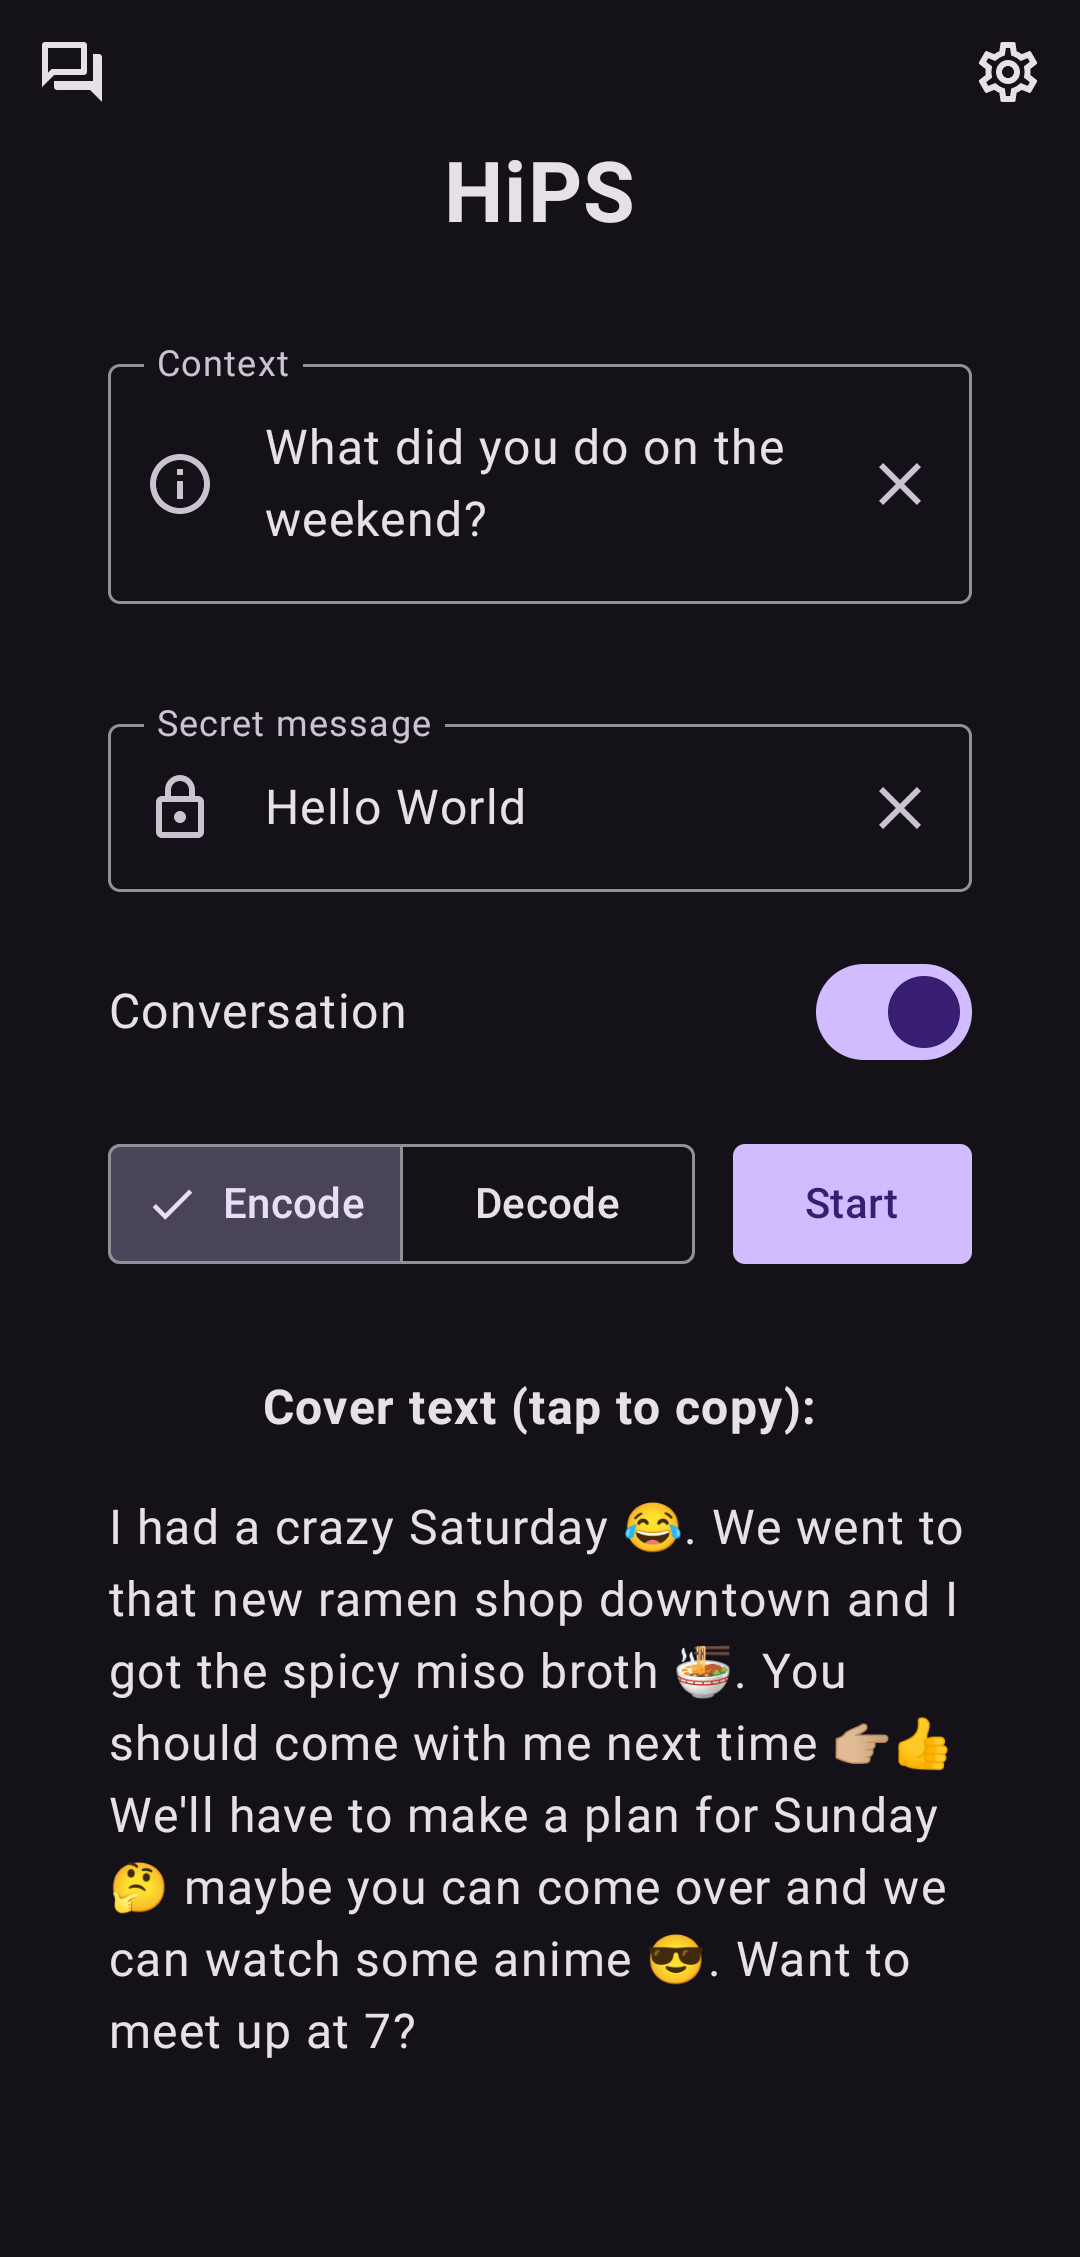
\includegraphics[width=\linewidth]{hips_home_screen_a.png}
			\caption{Encoding of a secret message.}
			\label{fig:homeScreenA}
		\end{subfigure}
        \hfill
		\begin{subfigure}{0.45\linewidth}
			\centering
			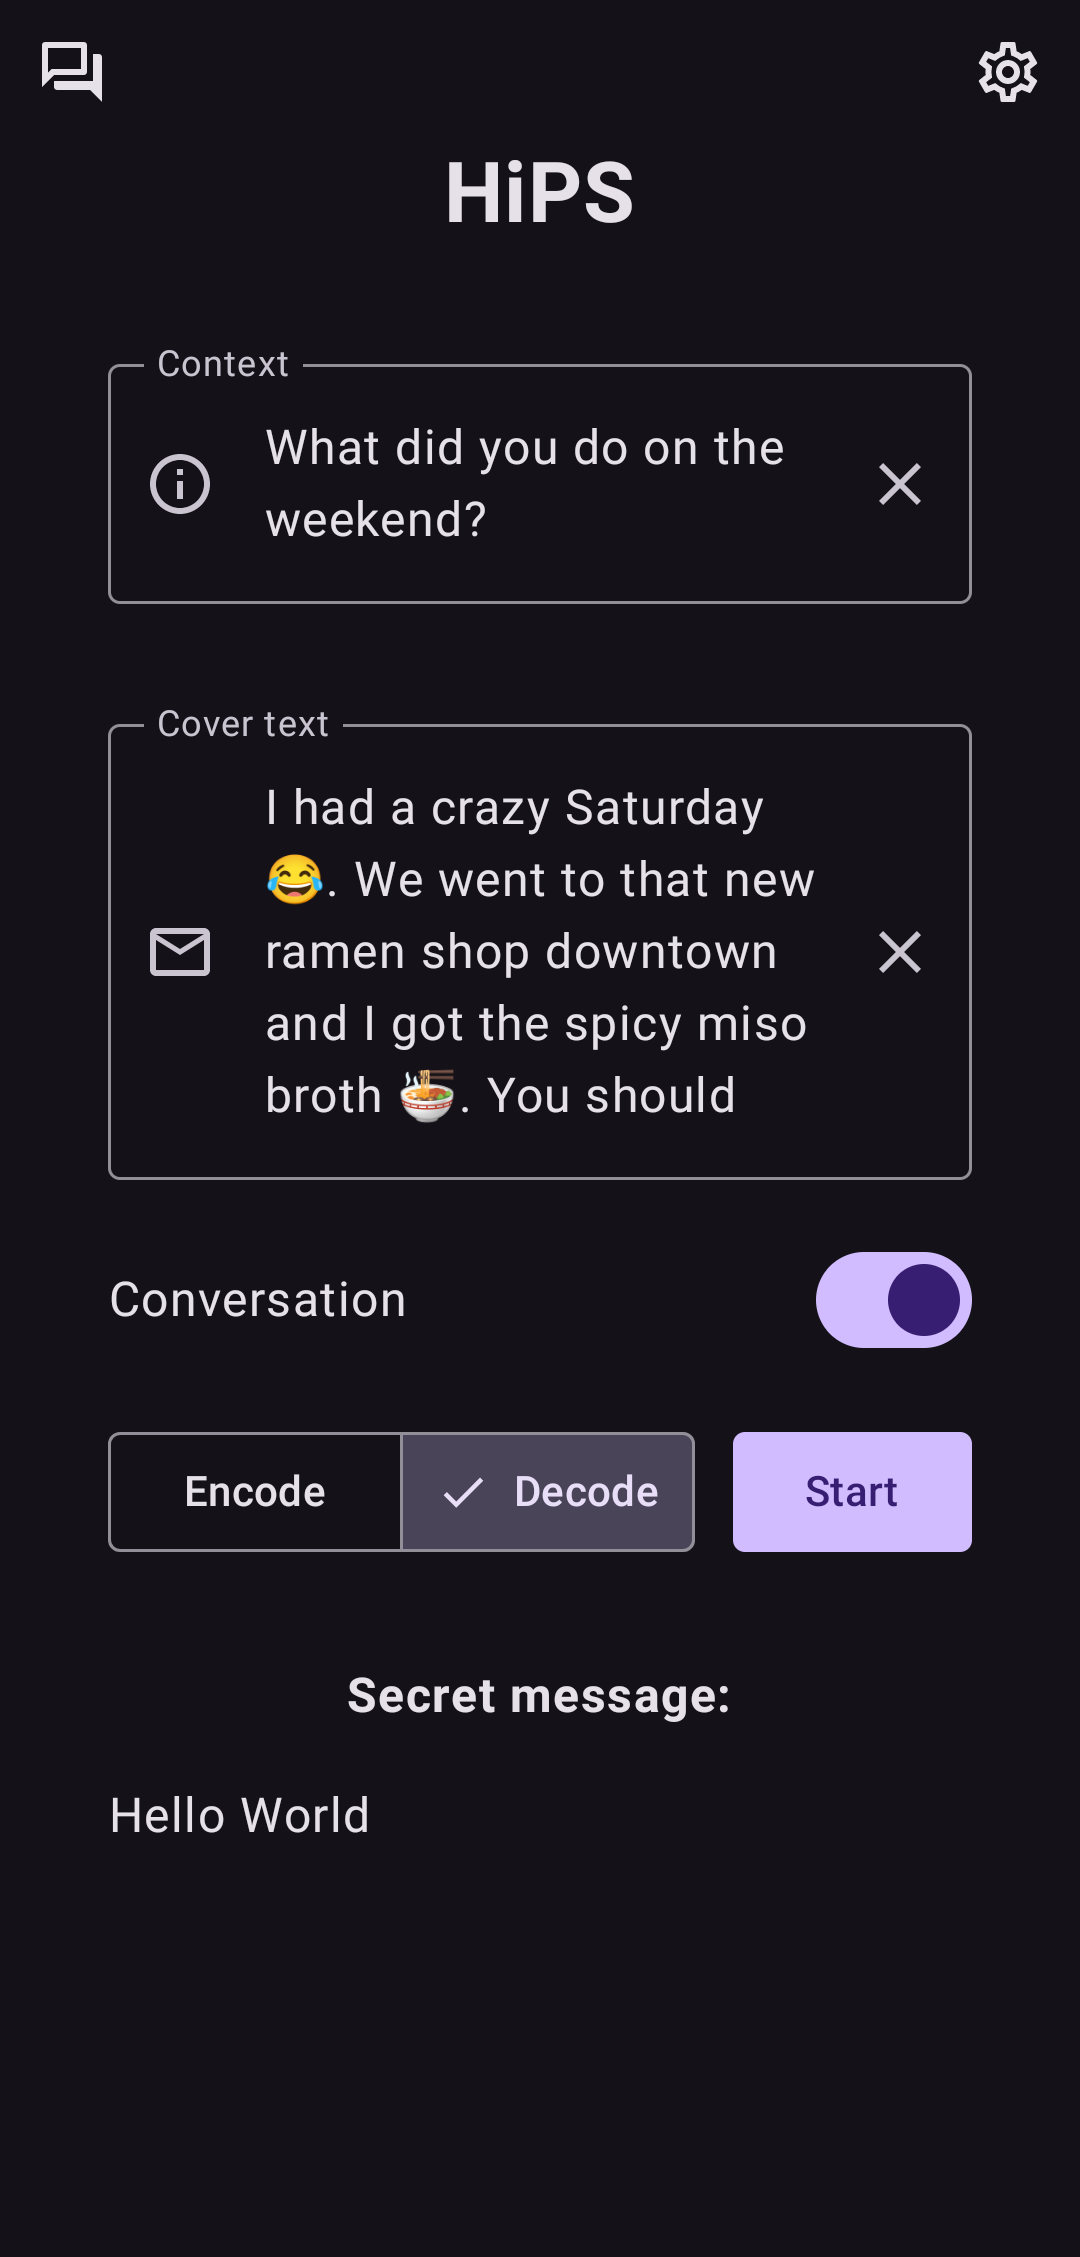
\includegraphics[width=\linewidth]{hips_home_screen_b.png}
			\caption{Decoding of a cover text.}
			\label{fig:homeScreenB}
		\end{subfigure}
		\caption[HiPS: Home screen]{Standalone functionality of HiPS on the home screen.}
		\label{fig:homeScreen}
	\end{wide}
\end{figure}

In encode mode, the input fields are for the context to generate a cover text from, and for the secret message to encode in the cover text. After pressing the start button, the cover text will be generated and displayed at the bottom. Tapping it copies it to the clipboard. In decode mode, the input fields are for the context and the cover text. After pressing the start button, the secret message will be displayed at the bottom.

The functionality of Stegasuras is replicated by toggling the conversation switch off. The cover text is then generated by \textit{completing} the context. This opens up adjacent use cases, e.g. generating a social media post to encode a secret message. When the conversation switch is toggled on, the functionality of Stegasuras is extended. The cover text is then generated by \textit{replying to} the context, i.e. the context is assumed to be a chat message. By offering this standalone functionality, we help users protect their privacy with existing instant messengers by simply copy-pasting their messages.

\subsection{Conversation screen}
\label{sec:conversationScreen}
\cref{fig:conversationScreen} shows the conversation screen. This is a demonstration of how steganography could be integrated into an instant messenger. This screen displays a list of messages, an input field and a send button. The messages are arranged as a chat conversation between two people and coloured accordingly. The input field allows the user to type in a new message, which can then be sent into the chat by pressing the send button. As this is a demo, messages are not being sent over the internet, but only stored locally. Effectively, users chat with themselves by constantly switching roles.

\begin{figure}
	\begin{wide}
		\captionsetup{width=\linewidth}
		\begin{subfigure}{0.45\linewidth}
			\centering
			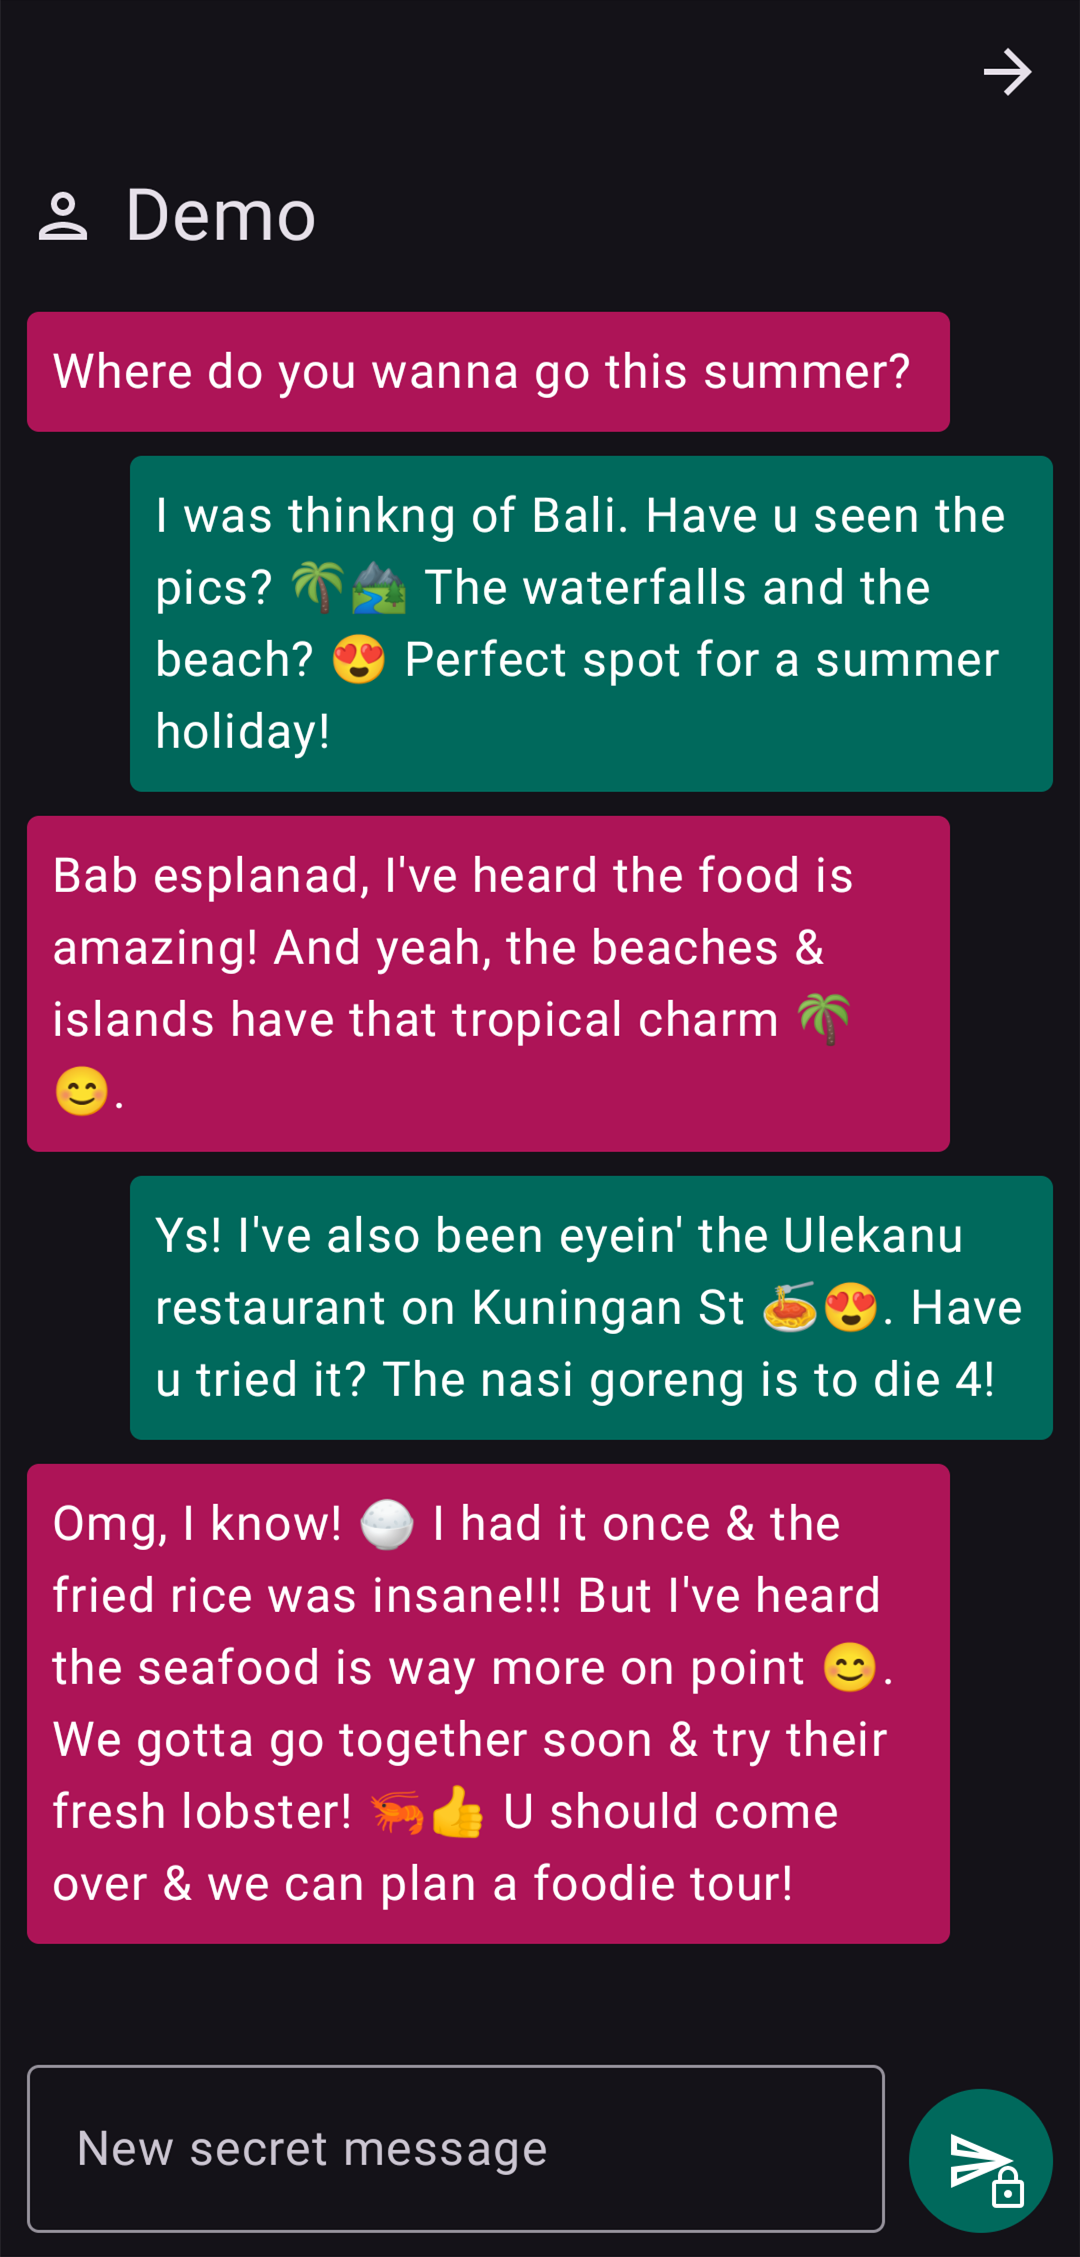
\includegraphics[width=\linewidth]{hips_conversation_screen_a.png}
			\caption{A conversation of cover texts.}
			\label{fig:conversationScreenA}
		\end{subfigure}
        \hfill
		\begin{subfigure}{0.45\linewidth}
			\centering
			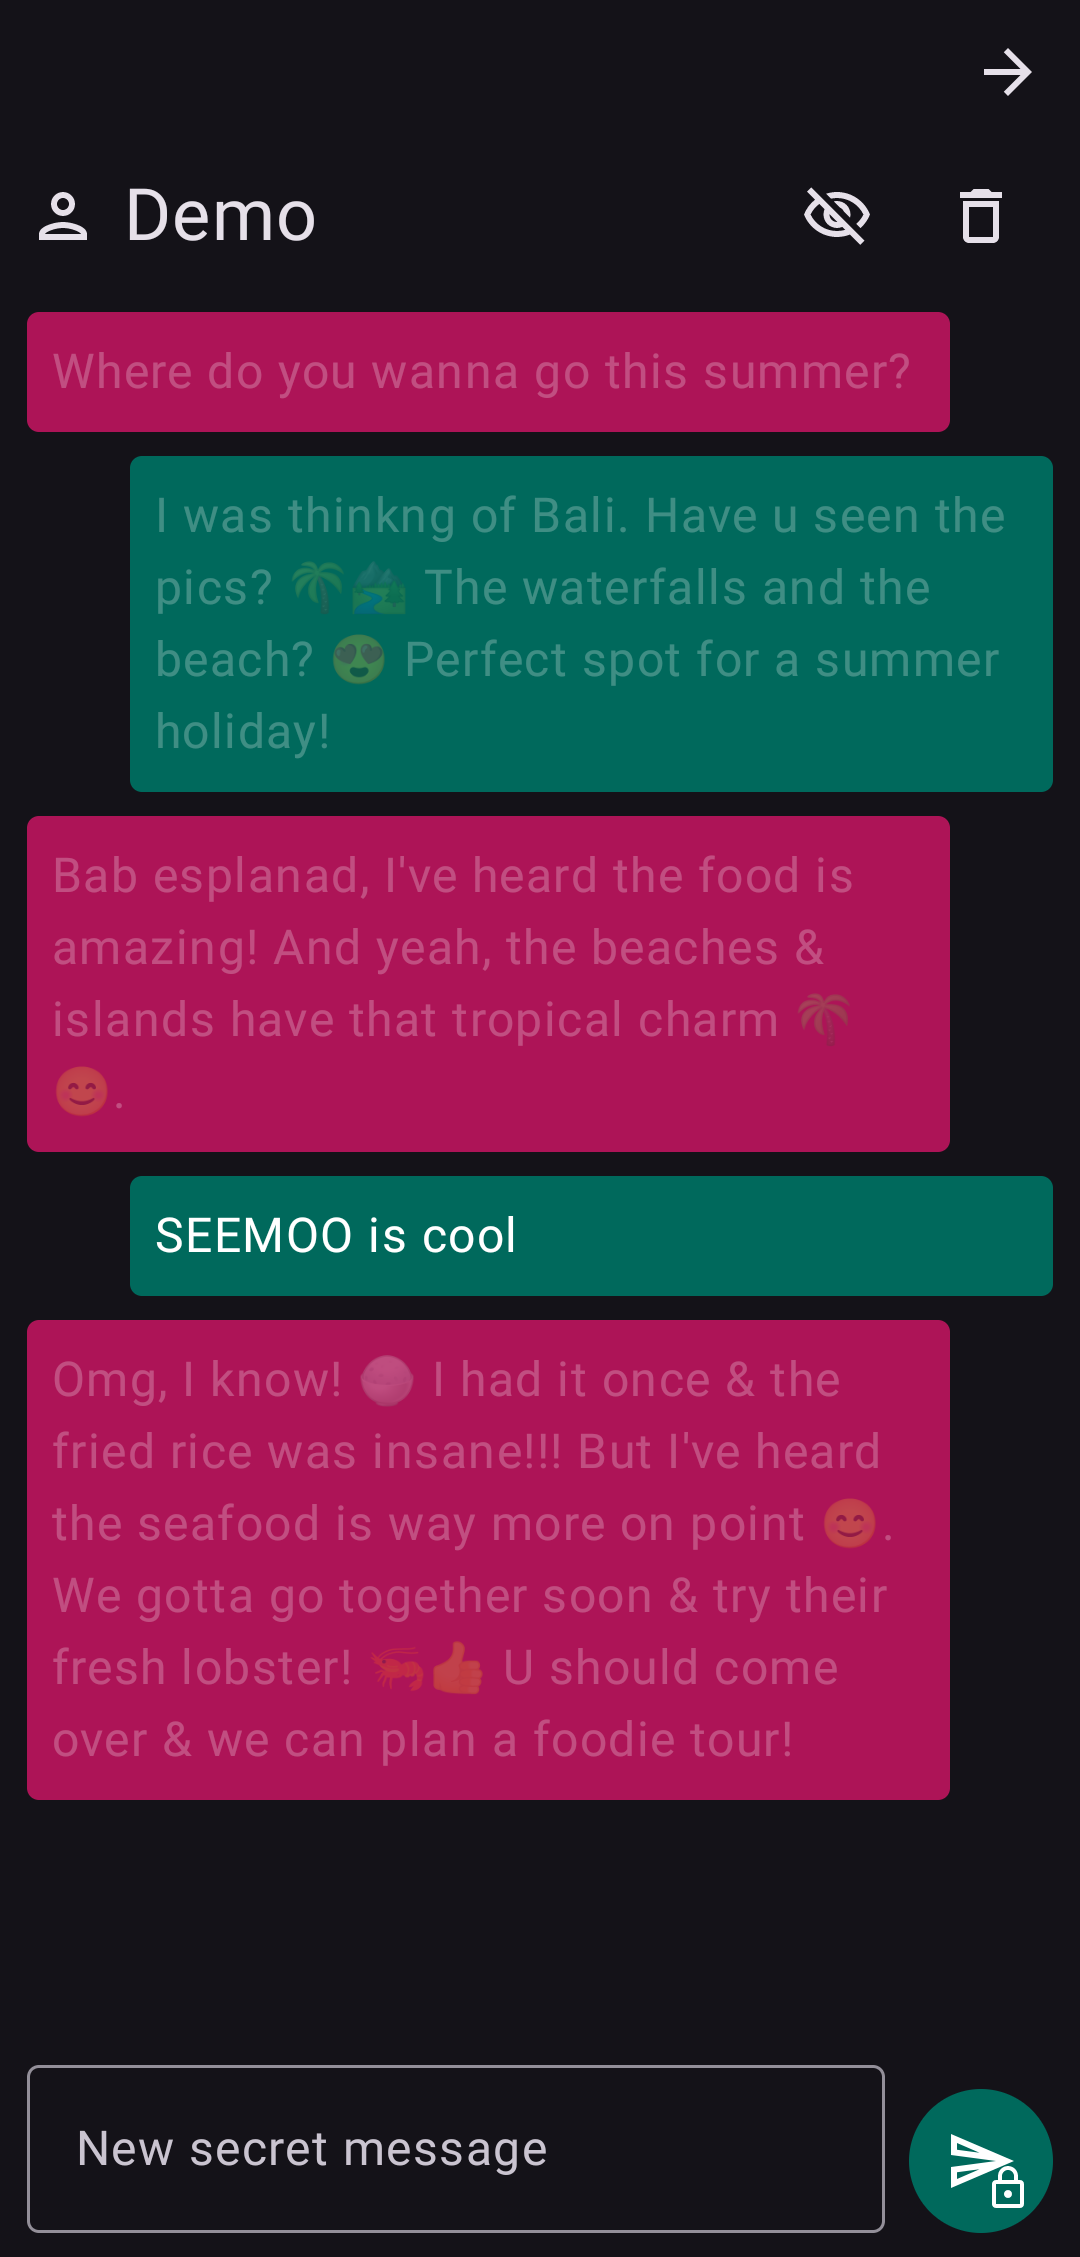
\includegraphics[width=\linewidth]{hips_conversation_screen_b.png}
			\caption{Showing a secret message.}
			\label{fig:conversationScreenB}
		\end{subfigure}
		\caption[HiPS: Conversation screen]{Steganography on the conversation screen.}
		\label{fig:conversationScreen}
	\end{wide}
\end{figure}

When the input field is blank, the send button can be short-pressed to switch roles. The current role is indicated by the send button being the same colour as the corresponding messages. This allows for sending multiple consecutive messages from the same role, i.e. for roles to not be strictly alternating. The role also switches automatically after sending a message.

The send button can be long-pressed to toggle steganography on/off. The current mode is indicated by a lock being shown or hidden inside it. If steganography is toggled on, the message in the input field is assumed to be a secret message and will be encoded into a cover text that replies to the conversation. This uses the prior messages as context. If steganography is toggled off, the message in the input field is assumed to be a plain text message and will be sent as is. This allows for arbitrary plain text messages in-between cover texts.

Messages in the chat can also be long-pressed, which highlights them as being selected. Short-pressing unselects them again. If at least one message is selected, two new buttons will be displayed at the top: Decode and delete.

The decode button can only be pressed if exactly one message is selected. This is to avoid running multiple instances of the \gls{LLM} simultaneously. Otherwise, the app process could be terminated by the Android operating system for excessive resource usage. When the decode button is pressed, it tries to decode the selected message. If decoding was successful (i.e. if the selected message was a cover text and not a plain text), the secret message will be displayed in place of the cover text. The symbol of the decode button changes to indicate that a secret message is visible. By pressing it again, the secret message and the two buttons are hidden again.

The delete button can only be pressed if the selected messages are at the end of the conversation. This is to avoid corrupting the context for decoding a message by deleting messages prior to it. When the delete button is pressed, the selected messages will be deleted and the two buttons will be hidden again.

\subsection{Settings screen}
\label{sec:settingsScreen}
\cref{fig:settingsScreen} shows the settings screen. This is where the \gls{LLM} is managed and where all parameters of our algorithms can be modified. Upon installation of our app, the user needs to download the \gls{LLM} by pressing the download button at the top of this screen. Then the \gls{LLM} can be loaded into or unloaded from memory by pressing the start/stop button below the download button. Pressing this button is only necessary after downloading the \gls{LLM} when using our app for the first time. Afterwards, the \gls{LLM} is automatically loaded on startup.

\begin{figure}
	\begin{wide}
		\captionsetup{width=\linewidth}
		\begin{subfigure}{0.45\linewidth}
			\centering
			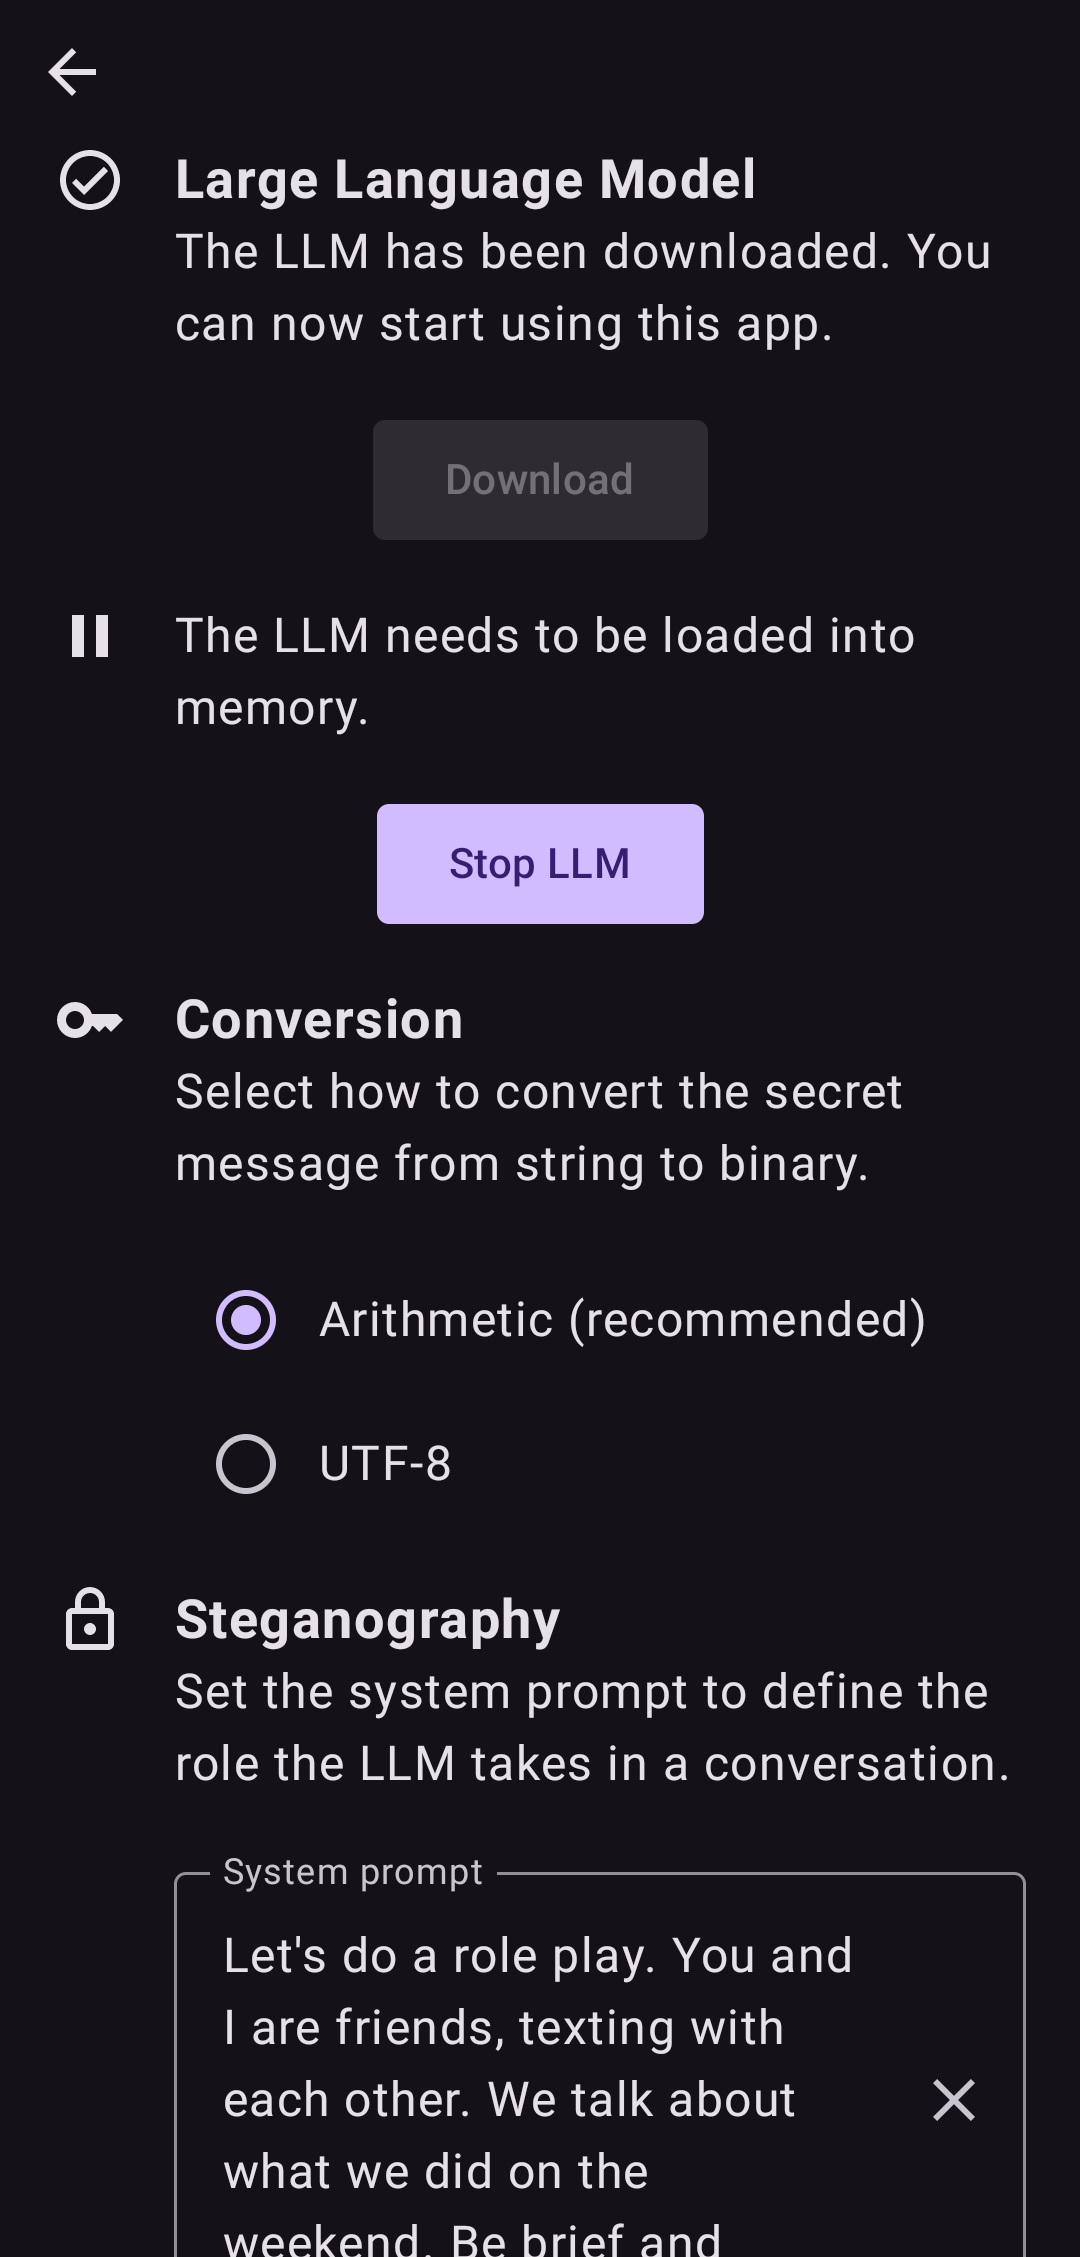
\includegraphics[width=\linewidth]{hips_settings_screen_a.png}
			\caption{Download button, start button, binary conversion mode, and system prompt.}
			\label{fig:settingsScreenA}
		\end{subfigure}
        \hfill
        \begin{subfigure}{0.45\linewidth}
			\centering
			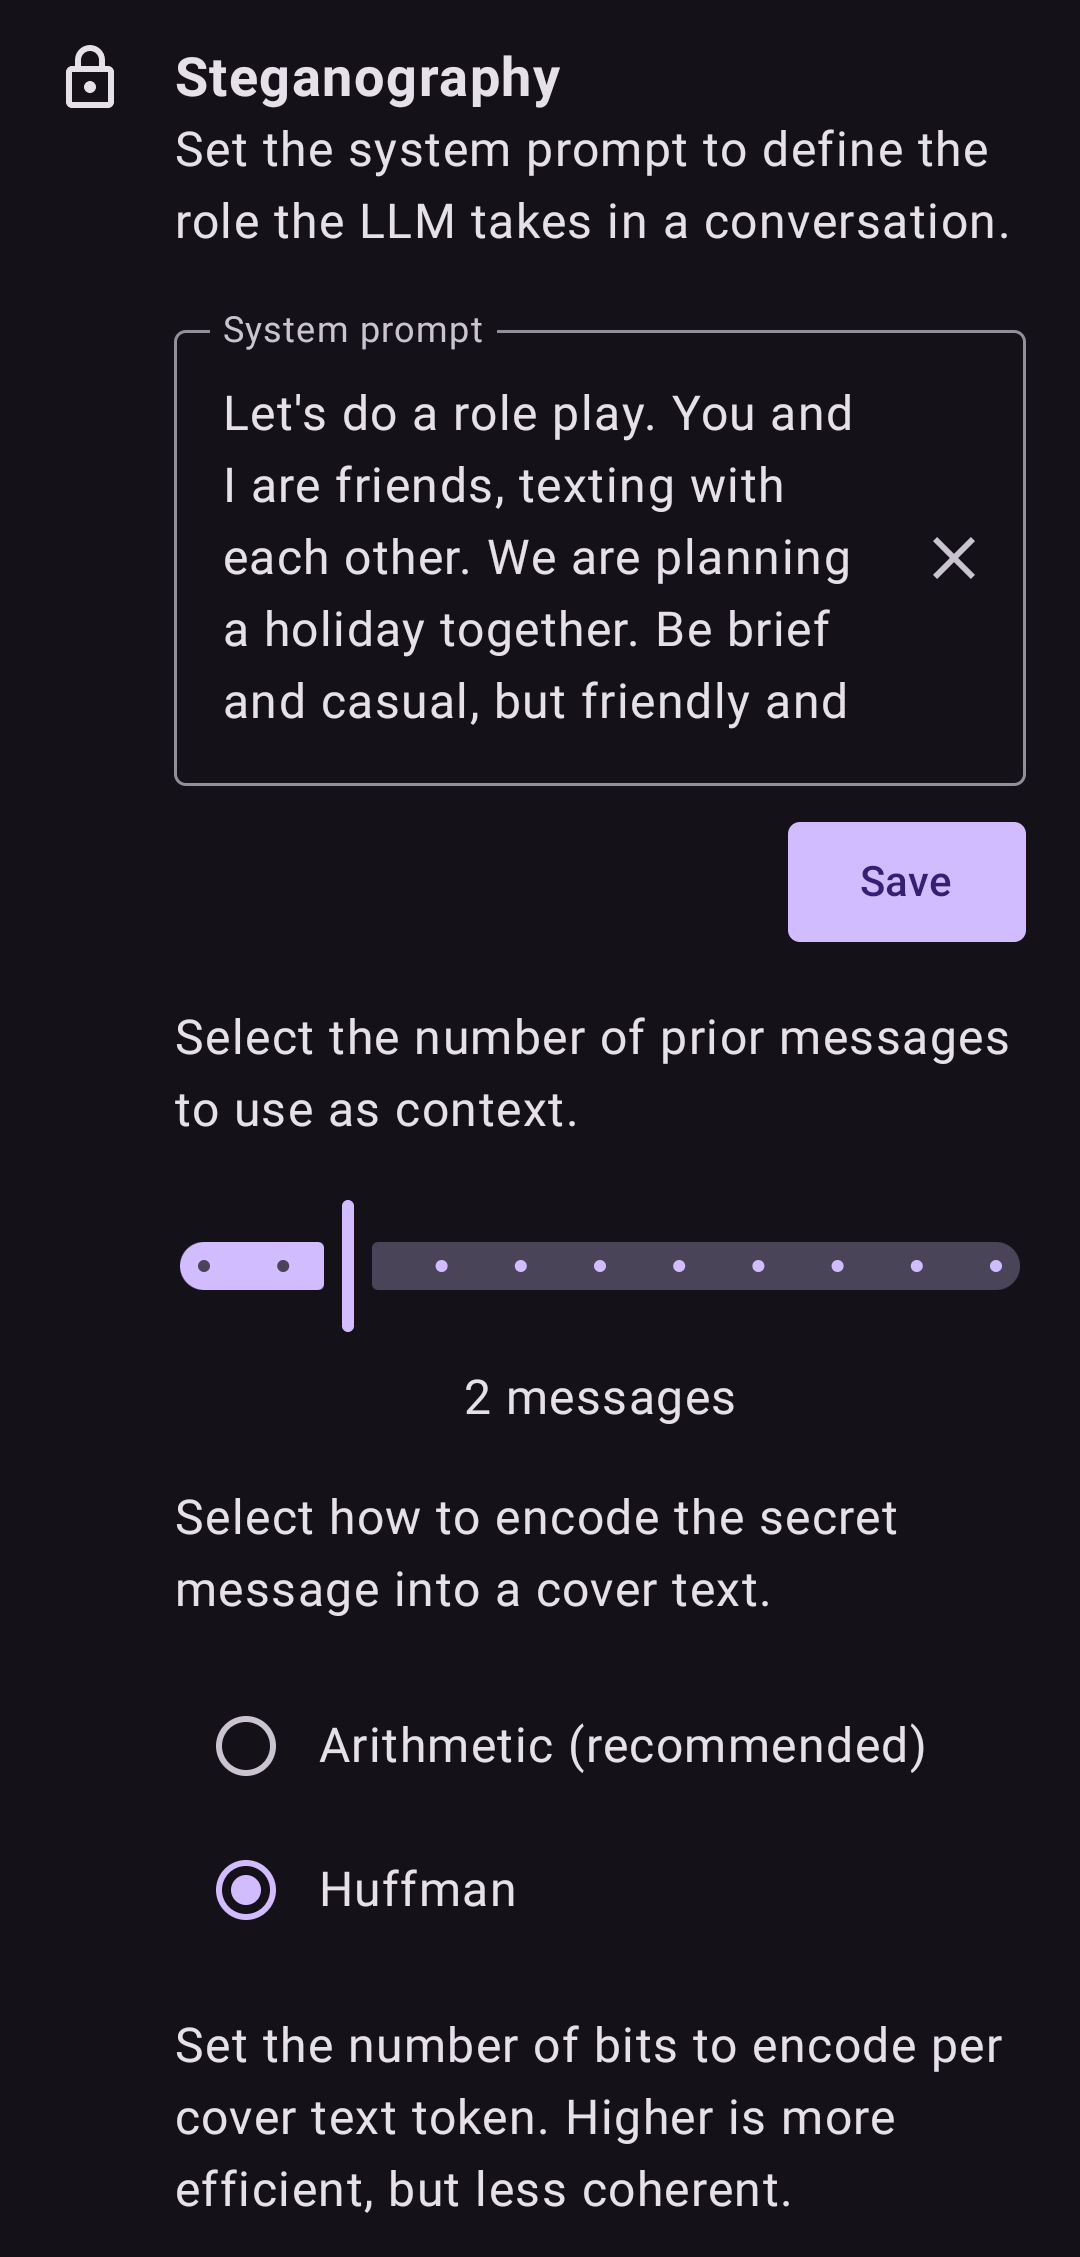
\includegraphics[width=\linewidth]{hips_settings_screen_b.png}
			\caption{Context length, steganography mode, parameters for Huffman coding, and reset options.}
			\label{fig:settingsScreenB}
		\end{subfigure}
		\caption[HiPS: Settings screen]{The settings screen.}
		\label{fig:settingsScreen}
	\end{wide}
\end{figure}

Below these buttons, there are various selectors, sliders and input fields for the parameters of our algorithms. They are arranged in the order of corresponding steps during the encoding of a secret message. First there is a selector for the conversion mode, i.e. for how to convert the secret message from string to binary. It offers \lstinline|Arithmetic (recommended)| and \lstinline|UTF-8| as options. \lstinline|UTF-8| serves as a baseline as it doesn't compress the secret message, while \lstinline|Arithmetic| compresses it using the \gls{LLM}.

This is followed by an input field for a system prompt. This is a natural language command that can be passed to the \gls{LLM} to influence its behaviour (see \cref{sec:creatingAConversationBetweenCoverTexts} for details). This is relevant for the conversation screen, and for the home screen if the conversation switch there is toggled on.

Afterwards, there is a slider to select a number of messages between 0 and 10. This is the number of prior messages to use as context on the conversation screen. While values 1 to 10 are used as is, 0 is interpreted as \lstinline|All messages|. This means all prior messages will be used as context to generate the next cover text from. We recommend setting this slider to a low value in the 1-10 range to limit resource usage.

Furthermore, we have a selector for the steganography algorithm. It offers \lstinline|Arithmetic (recommended)| and \lstinline|Huffman| as options. Parameters specific to the selected algorithm can be set using sliders below this selector (see \cref{sec:steganographyEncodingDecoding} for details): For \lstinline|Arithmetic|, there are three parameters called \lstinline|temperature|, \lstinline|topK| and \lstinline|precision|. Both \lstinline|topK| and \lstinline|precision| are only visible when the \gls{LLM} is in memory, as they are specific to the \gls{LLM}. For \lstinline|Huffman|, there is one parameter called \lstinline|bitsPerToken|.

Lastly, there is a button to reset all settings to their default values. It comes with a selector for whether to reset either only general settings, only settings that are specific to the \gls{LLM}, or both. When the \gls{LLM} is in memory, settings specific to it will be reset to sensible defaults. Otherwise, they are reset to 0.

\section{Java Native Interface}
\label{sec:javaNativeInterface}
We chose llama.cpp as the framework to run our \gls{LLM} with. Since this is a C++ library, we need a way to integrate C++ code into our Kotlin-based Android app. This is facilitated by the \gls{JNI}. It allows us to declare Kotlin functions as \lstinline|external|, signalling that their implementation is done in C++ rather than Kotlin. Arguments and return values can then be passed back and forth between Kotlin and C++.

Listings~\ref{lst:jniKotlin} and~\ref{lst:jniCpp} show examples for the Kotlin and C++ sides of the \gls{JNI}. On the Kotlin side, we implement the \lstinline|LlamaCpp| class to represent the \gls{LLM} instance. More specifically, \lstinline|LlamaCpp| is an \lstinline|object|. This is the Kotlin syntax for a singleton class. Multiple instances of the \gls{LLM} are avoided this way. On the C++ side, we only have implementations of functions declared \lstinline|external| in Kotlin, which generally are wrappers for llama.cpp function calls. Inputs and outputs need to be converted between Kotlin and C++ data types, but most logic is implemented in Kotlin. While this design decision may introduce performance drawbacks (see \cref{sec:performance}), it makes maintenance significantly easier.

% Add some space on top of listing to match bottom
\vspace{0.25cm}

\begin{lstlisting}[caption={[JNI: Kotlin side]{Example for the Kotlin side of the \gls{JNI}: State management for the \gls{LLM} using a function declared \lstinline|external| at the end.}}, label={lst:jniKotlin}]
object LlamaCpp {
    @Volatile
    private var model = 0L

    fun isInMemory(): Boolean {
        return model != 0L
    }

    fun startInstance() {
        if (isInMemory()) {
            return
        }

        synchronized(lock = this) {
            if (!isInMemory()) {
                model = loadModel()
            }
        }
    }

    private external fun loadModel(path: String): Long
}
\end{lstlisting}

% Move following paragraphs here to avoid page break in next listing
On the Kotlin side, the \gls{LLM} is loaded into memory by calling the \lstinline|loadModel| function with the path to a \lstinline|.gguf| file as a string argument. This function is declared \lstinline|external|, so its implementation is in C++. On the C++ side, the Kotlin string is converted to a C++ string via the \gls{JNI}. In turn, the \lstinline|llama_model_load_from_file| function of llama.cpp is called, which takes the file path as C++ string and some default parameters as arguments. This returns the memory address of the \gls{LLM} as a pointer. Pointers only exist in C++, but can be cast to Kotlin long numbers as both are 64 bits in size. Therefore, \lstinline|loadModel| returns a Kotlin long number. This is stored in the attribute \lstinline|model| of the \lstinline|LlamaCpp| object, so the state of the \gls{LLM} can be managed: If \lstinline|model| is \lstinline|0L|, the \gls{LLM} is not in memory. Otherwise it is and can be referenced via this attribute.

This enables us to implement any further logic in Kotlin. For example, the \lstinline|startInstance| function shown in Listing~\ref{lst:jniKotlin} loads of the \gls{LLM} in a thread-safe manner by implementing a double-checked locking mechanism~\cite{ishizakiTransformingJavaPrograms2014}. This is commonly used with singleton classes in Java, and by extension, Kotlin. Unloading the \gls{LLM} mirrors this. Other interactions with the \gls{LLM} are implemented similarly.

% Add some space on top of listing to match bottom
\vspace{0.25cm}

\begin{lstlisting}[caption={[JNI: C++ side]{Example for the C++ side of the \gls{JNI}: Implementation of the function declared \lstinline|external| in Listing~\ref{lst:jniKotlin}.}}, label={lst:jniCpp}]
extern "C" JNIEXPORT jlong JNICALL Java_org_vonderheidt_hips_utils_LlamaCpp_loadModel(JNIEnv* env, jobject /* thiz */, jstring jPath) {
    jboolean isCopy = true;

    const char* cppPath = env -> GetStringUTFChars(jPath, &isCopy);

    llama_model_params params = llama_model_default_params();

    llama_model* cppModel = llama_model_load_from_file(cppPath, params);

    env -> ReleaseStringUTFChars(jPath, cppPath);

    auto jModel = reinterpret_cast<jlong>(cppModel);

    return jModel;
}
\end{lstlisting}

\section{Token generation with llama.cpp}
\label{sec:tokenGenerationWithLlamaCpp}
\gls{HiPS} uses the popular llama.cpp framework to run \glspl{LLM} locally. We explain how token generation works with llama.cpp, i.e. how the \gls{LLM} generates text. We focus on the abstractions needed to work with llama.cpp, omitting any more general concepts. Most of this explanation is based on a great blog post by Omri Mallis~\cite{mallisUnderstandingHowLLM2023} and the examples given in the llama.cpp GitHub repository~\cite{gerganovGgerganovLlamacpp2024}. \cref{fig:llamaCppHighLevelFlow} shows the high-level flow we need to understand.

\begin{figure}
    \begin{wide}
        \captionsetup{width=\linewidth}
        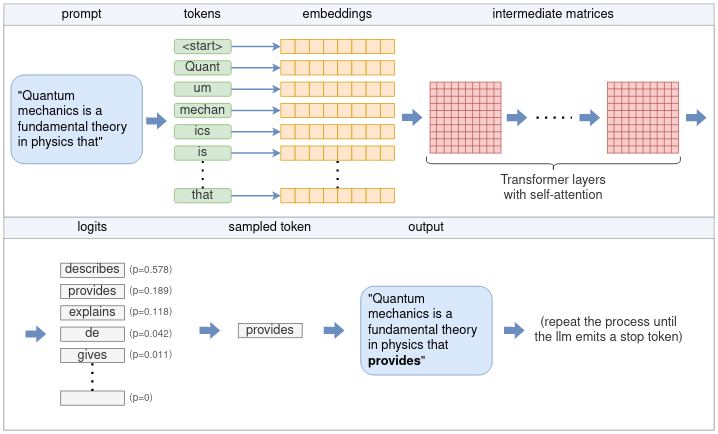
\includegraphics[width=\linewidth]{llama_cpp_high_level_flow.png}
        \caption[llama.cpp: Token generation]{High-level flow of token generation in llama.cpp. Taken from~\cite{mallisUnderstandingHowLLM2023}.}
        \label{fig:llamaCppHighLevelFlow}
    \end{wide}
\end{figure}

Fundamentally, \glspl{LLM} iteratively complete any text they are given as input~\cite{mallisUnderstandingHowLLM2023}. We call this input a prompt. The generated completion is returned as output. We call this output the response. In \cref{fig:llamaCppHighLevelFlow}, the prompt is "Quantum mechanics is a fundamental theory of physics that" and the response after one iteration is "provides"~\cite{mallisUnderstandingHowLLM2023}. The following paragraphs will explain what happens that iteration.

First, we need to understand an important distinction: The \gls{LLM} and its state. In the llama.cpp source code, the \gls{LLM} is called \lstinline|model|. Its state is called \lstinline|ctx| (short for context)~\cite{gerganovGgerganovLlamacpp2024}. The \lstinline|model| itself is stateless. This can be demonstrated by its idempotence: Consider one instance of a \lstinline|model| with an empty \lstinline|ctx|. When it is given a prompt, it will return a response. Reset the \lstinline|ctx| so it is empty again. If you give it the same prompt now, you will receive the same response again. Resetting the \lstinline|ctx| is important in our implementation to ensure reproducible results.

A \lstinline|ctx| takes the memory address of a \lstinline|model| as argument when being created~\cite{gerganovGgerganovLlamacpp2024}. Thereby, it is attached to the \lstinline|model| instance. Token generation only needs to access the \lstinline|ctx|. Resetting the \lstinline|ctx| works by unloading it from memory and loading a new \lstinline|ctx| attached to the same \lstinline|model| instance into memory. The implementation is analogous to loading and unloading the \gls{LLM} as shown in \cref{sec:javaNativeInterface}. However, the following paragraphs will only refer to the \gls{LLM} for readability, abstracting the \lstinline|ctx| away.

The \gls{LLM} starts processing the prompt by tokenizing it. This means that the prompt is not just split into words, but dismantled further into sub-word units called tokens~\cite{mallisUnderstandingHowLLM2023}. In \cref{fig:llamaCppHighLevelFlow}, for example the word "Quantum" is composed of the tokens "Quant" and "um". A token can be represented as a string, which is depicted in~\cref{fig:llamaCppHighLevelFlow}, or as an integer, which is then called the token ID~\cite{mallisUnderstandingHowLLM2023}. After tokenization, the \gls{LLM} works with token IDs. But for readability, we will mostly refer to them as tokens.

A common tokenization algorithm is \gls{BPE}~\cite{sennrichNeuralMachineTranslation2016}. Popular tokenizers using \gls{BPE} include Google's SentencePiece~\cite{googleGoogleSentencepiece2024}, which is used in Stegasuras~\cite{zieglerHarvardnlpNeuralSteganography2025,zieglerStegasuras2025}, and OpenAI's TikToken~\cite{openaiOpenaiTiktoken2025}, which is used in our \gls{LLM} of choice, Llama 3.2 1B~\cite{metaMetallamaLlamamodels2025}.

In llama.cpp, the tokens to be processed are stored in a separate data structure called a \lstinline|batch|. During the first iteration, the batch contains all tokens of the prompt. During subsequent iterations, the batch only contains the last sampled token~\cite{gerganovGgerganovLlamacpp2024}.

To complete the prompt, the \gls{LLM} needs to predict which tokens are likely to come next. To be comparable, the tokens need to be converted into a more structured representation. Each token in the prompt is converted into a vector, called an embedding~\cite{mallisUnderstandingHowLLM2023}. These vectors are then stacked to form the embedding matrix~\cite{mallisUnderstandingHowLLM2023}. \cref{fig:llamaCppEmbedding} shows the embedding matrix in detail. Its dimensions are \lstinline|n_tokens| $\times$ \lstinline|n_embd|. \lstinline|n_tokens| is the number of tokens in the prompt. \lstinline|n_embd| is the dimension of the vectors representing the tokens, which is specific to the \gls{LLM}~\cite{mallisUnderstandingHowLLM2023}.

\begin{figure}
    \begin{wide}
        \centering
        \captionsetup{width=\linewidth}
        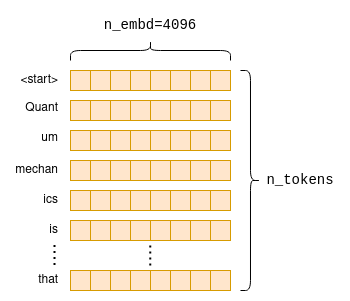
\includegraphics[width=0.5\linewidth]{llama_cpp_embedding.png}
        \caption[llama.cpp: Embedding matrix]{Details of the embedding matrix in llama.cpp. \lstinline|n_embd| is specific to the \gls{LLM} (the value depicted here is for Llama 2). Taken from~\cite{mallisUnderstandingHowLLM2023}.}
        \label{fig:llamaCppEmbedding}
    \end{wide}
\end{figure}

With the prompt effectively converted into a matrix representation, the \gls{LLM} can now apply \textit{transformations} to it, i.e. multiply it with a series of matrices. \cref{fig:llamaCppHighLevelFlow} depicts this as "Transformer layers with self-attention". This is the core of the \textit{Transformer} architecture, which is the basis for most \glspl{LLM} today~\cite{vaswaniAttentionAllYou2023}. Different variants of the Transformer architecture exist, namely encoder-decoder or decoder-only~\cite{mallisUnderstandingHowLLM2023}. They each come with their own strengths and weaknesses, the discussion of which is out of scope for this thesis. For us, it is only relevant that we want to support as many \glspl{LLM} as possible. This means we have to check if an encoding step is required before performing the decoding step. Fortunately, llama.cpp abstracts this away behind a simple function call each~\cite{gerganovGgerganovLlamacpp2024}. This was shown earlier in Listing~\ref{lst:llamaCpp}. The result of these transformations is a matrix of logits, i.e. of unnormalized probabilities for the prediction of the next token~\cite{mallisUnderstandingHowLLM2023}. \cref{fig:llamaCppLogits} shows the logits matrix in detail. Its dimensions are \lstinline|n_tokens| $\times$ \lstinline|n_vocab|. \lstinline|n_vocab| is the vocabulary size specific to the \gls{LLM}, i.e. the number of tokens it knows~\cite{mallisUnderstandingHowLLM2023}.

\begin{figure}
    \begin{wide}
        \captionsetup{width=\linewidth}
        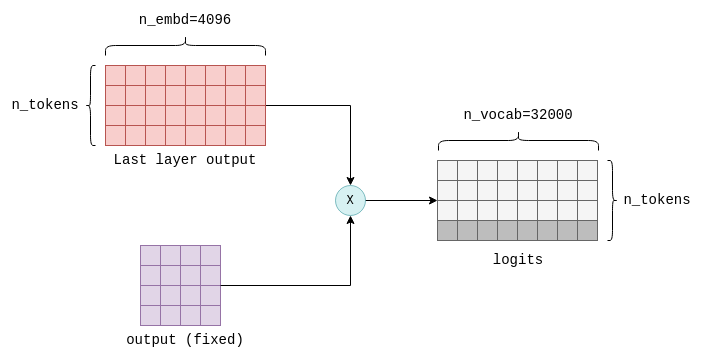
\includegraphics[width=\linewidth]{llama_cpp_logits.png}
        \caption[llama.cpp: Logit matrix]{Details of the logit matrix in llama.cpp. Also shown is the last transformation layer, i.e. the last intermediate matrix being multiplied with a fixed "output" matrix. This is not to be confused with the output of the \gls{LLM} as defined earlier. Taken from~\cite{mallisUnderstandingHowLLM2023}.}
        \label{fig:llamaCppLogits}
    \end{wide}
\end{figure}

Each row of the logit matrix corresponds to a token in the prompt. It contains the logits for every token in the vocabulary to follow this token of the prompt. In other words, only the last row of the logit matrix is relevant for us, as it contains the logits for the last token of the prompt~\cite{mallisUnderstandingHowLLM2023}. This is highlighted in \cref{fig:llamaCppLogits}. Generally, these logits will be normalized using a softmax function (see \cref{sec:theGenericAlgorithm} for details). Only then they are interpretable as probabilities~\cite{mallisUnderstandingHowLLM2023,turnerIntroductionTransformers2024}.

Now we need to sample a token to complete the prompt with, based on the probabilities we just calculated~\cite{mallisUnderstandingHowLLM2023}. We will implement our own sampling logic to perform steganography, i.e. to encode a secret message into a cover text by sampling certain tokens (see \cref{sec:arithmeticCoding,sec:huffmanCoding} for details). To do this, we need to understand several general-purpose sampling methods. The simplest is called greedy sampling. Greedy sampling always selects the token with the highest probability~\cite{mallisUnderstandingHowLLM2023}. Other common approaches are temperature sampling and top-k sampling~\cite{mallisUnderstandingHowLLM2023}. In temperature sampling, the probabilities are scaled with $1/temperature$ to modify their distribution. For $temperature < 1$, the distribution gets steeper around the most likely token. This makes the \gls{LLM} responses more coherent. For $temperature > 1$, the distribution gets flatter. This makes the \gls{LLM} responses less coherent ("more creative")~\cite{mallisUnderstandingHowLLM2023}. Top-k sampling only considers the tokens with the k highest probabilities~\cite{mallisUnderstandingHowLLM2023}.

When a token is sampled, it is appended to the prompt to construct the response~\cite{mallisUnderstandingHowLLM2023}. The full response is built iteratively, so this output is used as input for the next iteration. This is also called autoregressive~\cite{mallisUnderstandingHowLLM2023}. Iteration stops when the \gls{LLM} samples a special end-of-generation token~\cite{gerganovGgerganovLlamacpp2024}. While the response in principle is ready now, it is still represented as token IDs. Before being displayed to the user as a string, it needs to be detokenized~\cite{mallisUnderstandingHowLLM2023}. The response after one iteration is shown in \cref{fig:llamaCppHighLevelFlow}, after sampling the token "provides".

\section{Algorithms}
\label{sec:algorithms}
Based on the Stegasuras project~\cite{zieglerNeuralLinguisticSteganography2019}, we implement algorithms to perform steganography in two steps:
\begin{itemize}
    \item Convert the secret message from string to binary, compressing it in the process.
    \item Generate a cover text by completing a given context with the \gls{LLM}, thereby encoding the secret message bits.
\end{itemize}

This can be viewed as a generic algorithm with exchangeable implementations for each of the two steps. For the first step, we implement UTF-8 conversion and Arithmetic compression. For the second step, we implement Huffman coding and Arithmetic coding\footnote{Stegasuras implements another algorithm called Bins coding. While Huffman and Arithmetic coding were on par in qualitative and quantitative steganalysis, Bins performed significantly worse~\cite{zieglerNeuralLinguisticSteganography2019}. Therefore, we don't implement it.}. We first discuss the generic algorithm, then the different implementations for each step. This is intended as a high-level overview to support documentation of our code.

\subsection{The generic algorithm}
\label{sec:theGenericAlgorithm}
The steganography algorithms demonstrated by Stegasuras~\cite{zieglerNeuralLinguisticSteganography2019} can be viewed as different implementations of a single generic algorithm: They differ only in how the secret message is converted from string to binary and how its bits are encoded during the sampling of cover text tokens. We explain the generic algorithm here.

To \textbf{encode} the bits of a secret message into a cover text using a context, we tokenize the context first. We let the \gls{LLM} generate cover text tokens in a loop. This loop terminates when all bits are encoded and the last sentence of the cover text is finished. In every iteration, we let the \gls{LLM} calculate logits: First using the context tokens, then using the last cover text token we sampled. As logits can generally assume negative values, they need to be normalized to the $ [0, 1] $ interval to be interpretable as probabilities. This is done using softmax functions~\cite{turnerIntroductionTransformers2024}. \cref{eqn:softmax} shows a common softmax function ($p_i$ = probability of token i, $l_i$ = logit of token i, $n_{vocab}$ = vocabulary size of the \gls{LLM}). It applies the exponential function to the logits to transform them to non-negative values. This is suitable as the exponential function is strictly monotonous in growth, therefore maintaining the order of the associated tokens.

\begin{align}
	p_i = \frac{\exp(l_i)}{\sum_{j=1}^{n_{vocab}} \exp(l_j)}
	\label{eqn:softmax}
\end{align}

To avoid early termination, we need to manually suppress end-of-generation tokens by setting their probability to zero. Otherwise, we may render our secret message unrecoverable by not encoding all of its bits.

If there are secret message bits left to encode, the implementation-specific sampling logic is applied (see \cref{sec:arithmeticCoding,sec:huffmanCoding} for details). It samples the next cover text token based on the secret message bits and the probabilities we just calculated. Otherwise, greedy sampling is applied to finish the last sentence of the cover text. After the last iteration, the sampled cover text tokens are detokenized to return the cover text.

To \textbf{decode} a cover text back into secret message bits using a context, we calculate the same probabilities as during encoding: We tokenize both context and cover text. In a loop through the cover text tokens, we let the \gls{LLM} calculate logits. Again first using the context tokens, then using the current cover text token. Now we only need to inverse the implementation-specific sampling logic, deriving the secret message bits from the cover text tokens. After processing all cover text tokens, we return the binary secret message.

\subsection{Finishing the last sentence}
\label{sec:finishingTheLastSentence}
While we are able to use the generic algorithm demonstrated by Stegasuras~\cite{zieglerNeuralLinguisticSteganography2019} to perform steganography, it comes with an unsolved edge case: If cover text generation would end as soon as the secret message is encoded, its last sentence would most likely be incomplete. Not finishing the last sentence of a cover text is not an option, as it would make our communication highly suspicious to attackers. A possible solution is to perform greedy sampling until a suitable punctuation mark is reached. This is already demonstrated by Stegasuras~\cite{zieglerHarvardnlpNeuralSteganography2025}. But when we decode such a cover text, we get the secret message, followed by some noise. This is because the tokens from greedy sampling don't encode any actual information. If we left it like this, user experience of our app would be quite unpolished.

We propose a solution to clean up this noise during decoding: We inject a suitable stop signal during encoding by appending it to the secret message. During decoding, we can thereby identify the end of the secret message and cut off the stop signal and any noise that follows it. The challenge is finding a step in the encoding process that is suitable for injection, which also determines the form of the stop signal.

As the secret message may get encrypted between binary conversion and cover text generation, we cannot make any structural assumptions about the bits being \textit{decoded} from a cover text. Therefore we have to insert our stop signal earlier in the encoding process, so that we can identify it later in the decoding process.

This ultimately led us to consider a special character as a stop signal. We append this special character to the secret message before it gets converted from string to binary. A suitable special character needs to be unlikely as organic user input, so that blocking it doesn't degrade the user experience significantly. The ASCII NUL character presents such a solution. While languages such as C and C++ use it for string termination, it doesn't serve any purpose in Kotlin. As it doesn't have a visual representation, it is not on any standard keyboard. This enables us to clean up any noise in decoding with minimal overhead.

\subsection{UTF-8}
\label{sec:utf8}
To convert the secret message from string to binary, we implement UTF-8 encoding. We chose UTF-8 as it is the most popular Unicode encoding: Around 90\% of all text on the internet is encoded in UTF-8~\cite{gleaveMakingCompressionAlgorithms2017}. It doesn't compress the secret message, but represents every character with one to four bytes instead~\cite{gleaveMakingCompressionAlgorithms2017}. This makes cover texts significantly longer. Therefore, it serves as a baseline to compare Arithmetic compression to.

\subsection{Huffman coding}
\label{sec:huffmanCoding}
To encode the secret message into a cover text, we implement Huffman coding. Huffman coding is a steganography algorithm based on Huffman compression~\cite{zieglerNeuralLinguisticSteganography2019,yangRNNStegaLinguisticSteganography2019}. Huffman compression is popular because of its ability to compress data to near entropy~\cite{huffmanMethodConstructionMinimumRedundancy1952}.

First, we define some data structures. Huffman coding constructs a binary tree, the Huffman tree, which is composed of nodes~\cite{huffmanMethodConstructionMinimumRedundancy1952}. Each node can store a token, a probability, and its own left and right child nodes as attributes~\cite{huffmanMethodConstructionMinimumRedundancy1952}. Nodes are compared by probability~\cite{huffmanMethodConstructionMinimumRedundancy1952}.

We use a Java PriorityQueue to construct the Huffman tree iteratively. Initially, it only contains nodes that store tokens. In each iteration, we remove the two nodes with the lowest probabilities. We create a new parent node for them that stores the sum of their probabilities, but no token. The new node gets inserted back into the priority queue. Iteration ends when there is only one node left, which then becomes the root node of the Huffman tree~\cite{huffmanMethodConstructionMinimumRedundancy1952}. Only now is the Huffman tree a binary tree. Its leaf nodes store the tokens. Above them, the new nodes have been inserted. They don't store tokens, but store the cumulated probabilities of their sub-trees~\cite{huffmanMethodConstructionMinimumRedundancy1952}.

Each node gets assigned a Huffman code. We generate Huffman codes by traversing the Huffman tree from top to bottom, interpreting a left turn as a 0 bit and a right turn as a 1 bit~\cite{huffmanMethodConstructionMinimumRedundancy1952}.

Now we are ready to perform steganography via Huffman coding. We encode the bits of a secret message into a cover text by sampling specific tokens. This uses the probabilities calculated by the \gls{LLM} and one parameter as input: \lstinline|bitsPerToken|. This is an integer determining how many bits are encoded per cover text token. The output is the sampled cover text token.

Consider the tokens with the top $ 2^{bitsPerToken} $ probabilities. We construct a Huffman tree from them and generate the Huffman codes. Huffman codes of leaf nodes now all have the same length: \lstinline|bitsPerToken| bits, the height of the Huffman tree. We traverse the Huffman tree based on the secret message bits. If there are not enough bits left at the end, we go in one direction until we reach a leaf node\footnote{Any leaf node of the sub-tree reached after the last bit would be fine. The additional turns create artefacts similar to greedy sampling, but those are cleaned up in decoding (see \cref{sec:finishingTheLastSentence}).}. By sampling the token stored in the leaf node we arrive at after taking \lstinline|bitsPerToken| turns, we encode this number of bits. \cref{fig:huffmanCoding} shows an example Huffman tree for \lstinline|bitsPerToken| = 2 bits/token.

\begin{figure}
    \begin{wide}
        \centering
        \captionsetup{width=\linewidth}
        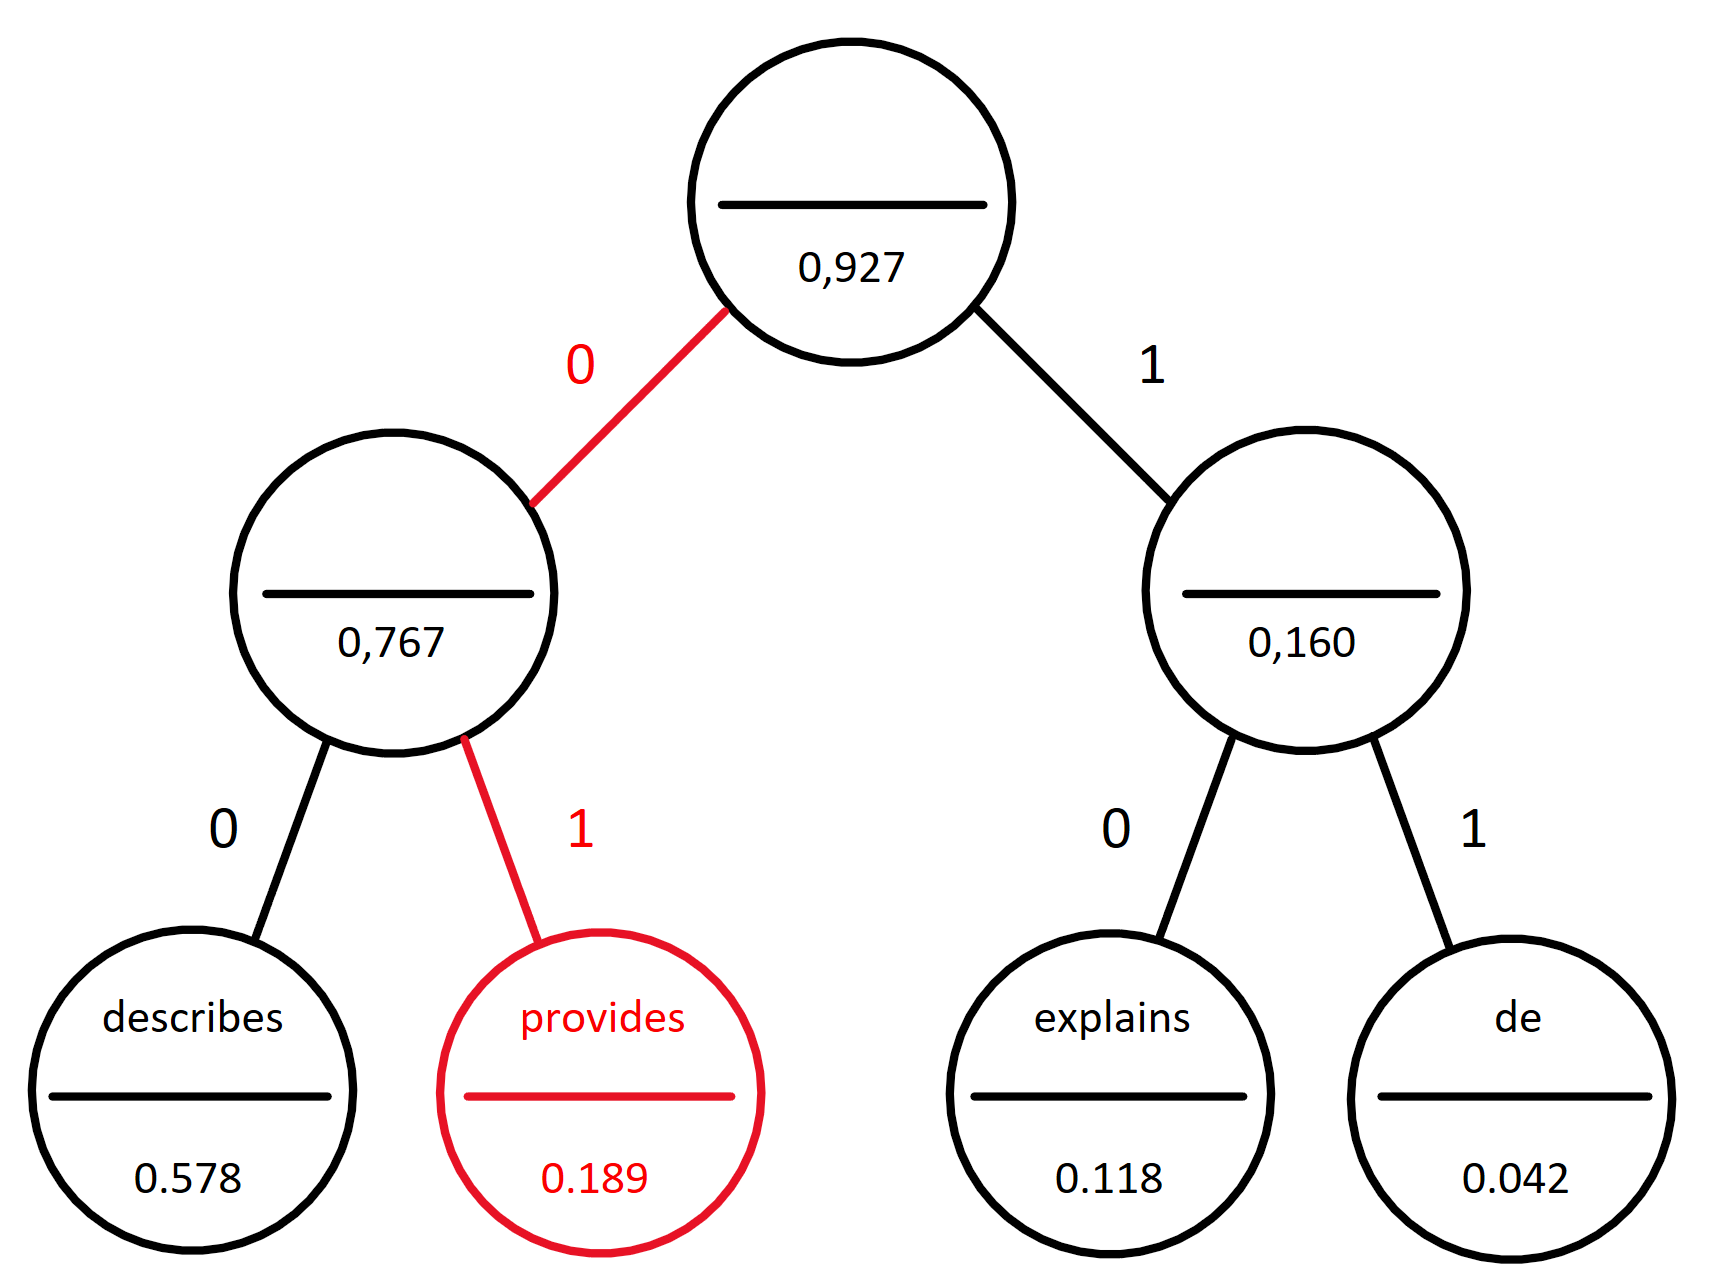
\includegraphics[width=0.67\linewidth]{huffman_coding.png}
		\caption[Huffman coding]{Example of a Huffman tree for \lstinline|bitsPerToken| = 2. Nodes are labelled with tokens and their probabilities, edges with the bits they are interpreted as during traversal. Highlighted is the path that would be taken when encoding the bits 01 of a secret message. The token "provides" would be sampled.}
        \label{fig:huffmanCoding}
    \end{wide}
\end{figure}

The last paragraph shows the simplicity of Huffman coding. We only need one parameter to control the trade-off between length and quality of cover texts. A low \lstinline|bitsPerToken| value (e.g. 1 bit/token) will only consider few most likely tokens, making the Huffman tree shallow. Cover texts will be long, but coherent. The inverse is true for a high \lstinline|bitsPerToken| value (e.g. 4 bits/token). However, Huffman coding also comes with a downside. It aims to maximize cover text quality at maximum compression~\cite{zieglerNeuralLinguisticSteganography2019}. This may be good enough to fool human eavesdroppers, but it is not sufficient to defend against machine-based attacks, as these can identify statistical patterns in cover texts~\cite{zieglerNeuralLinguisticSteganography2019}.

\subsection{Arithmetic coding}
\label{sec:arithmeticCoding}
To encode the secret message into a cover text, we implement Arithmetic coding. Arithmetic coding is based on a compression algorithm where data is represented as a decimal number in the $ [0, 1) $ interval. This is achieved by iteratively narrowing the boundaries: In every iteration, a sub-interval is selected based on a part of the data and divided into further sub-intervals~\cite{rissanenArithmeticCoding1979}. \cref{fig:arithmeticCoding} provides a visualization. Arithmetic coding is popular because of its ability to compress data to near entropy~\cite{rissanenArithmeticCoding1979}. Stegasuras implements a variant of this using wider integer intervals that don't strictly narrow down to perform steganography~\cite{zieglerNeuralLinguisticSteganography2019,rubinArithmeticStreamCoding1979}.

\begin{figure}
    \begin{wide}
        \captionsetup{width=\linewidth}
        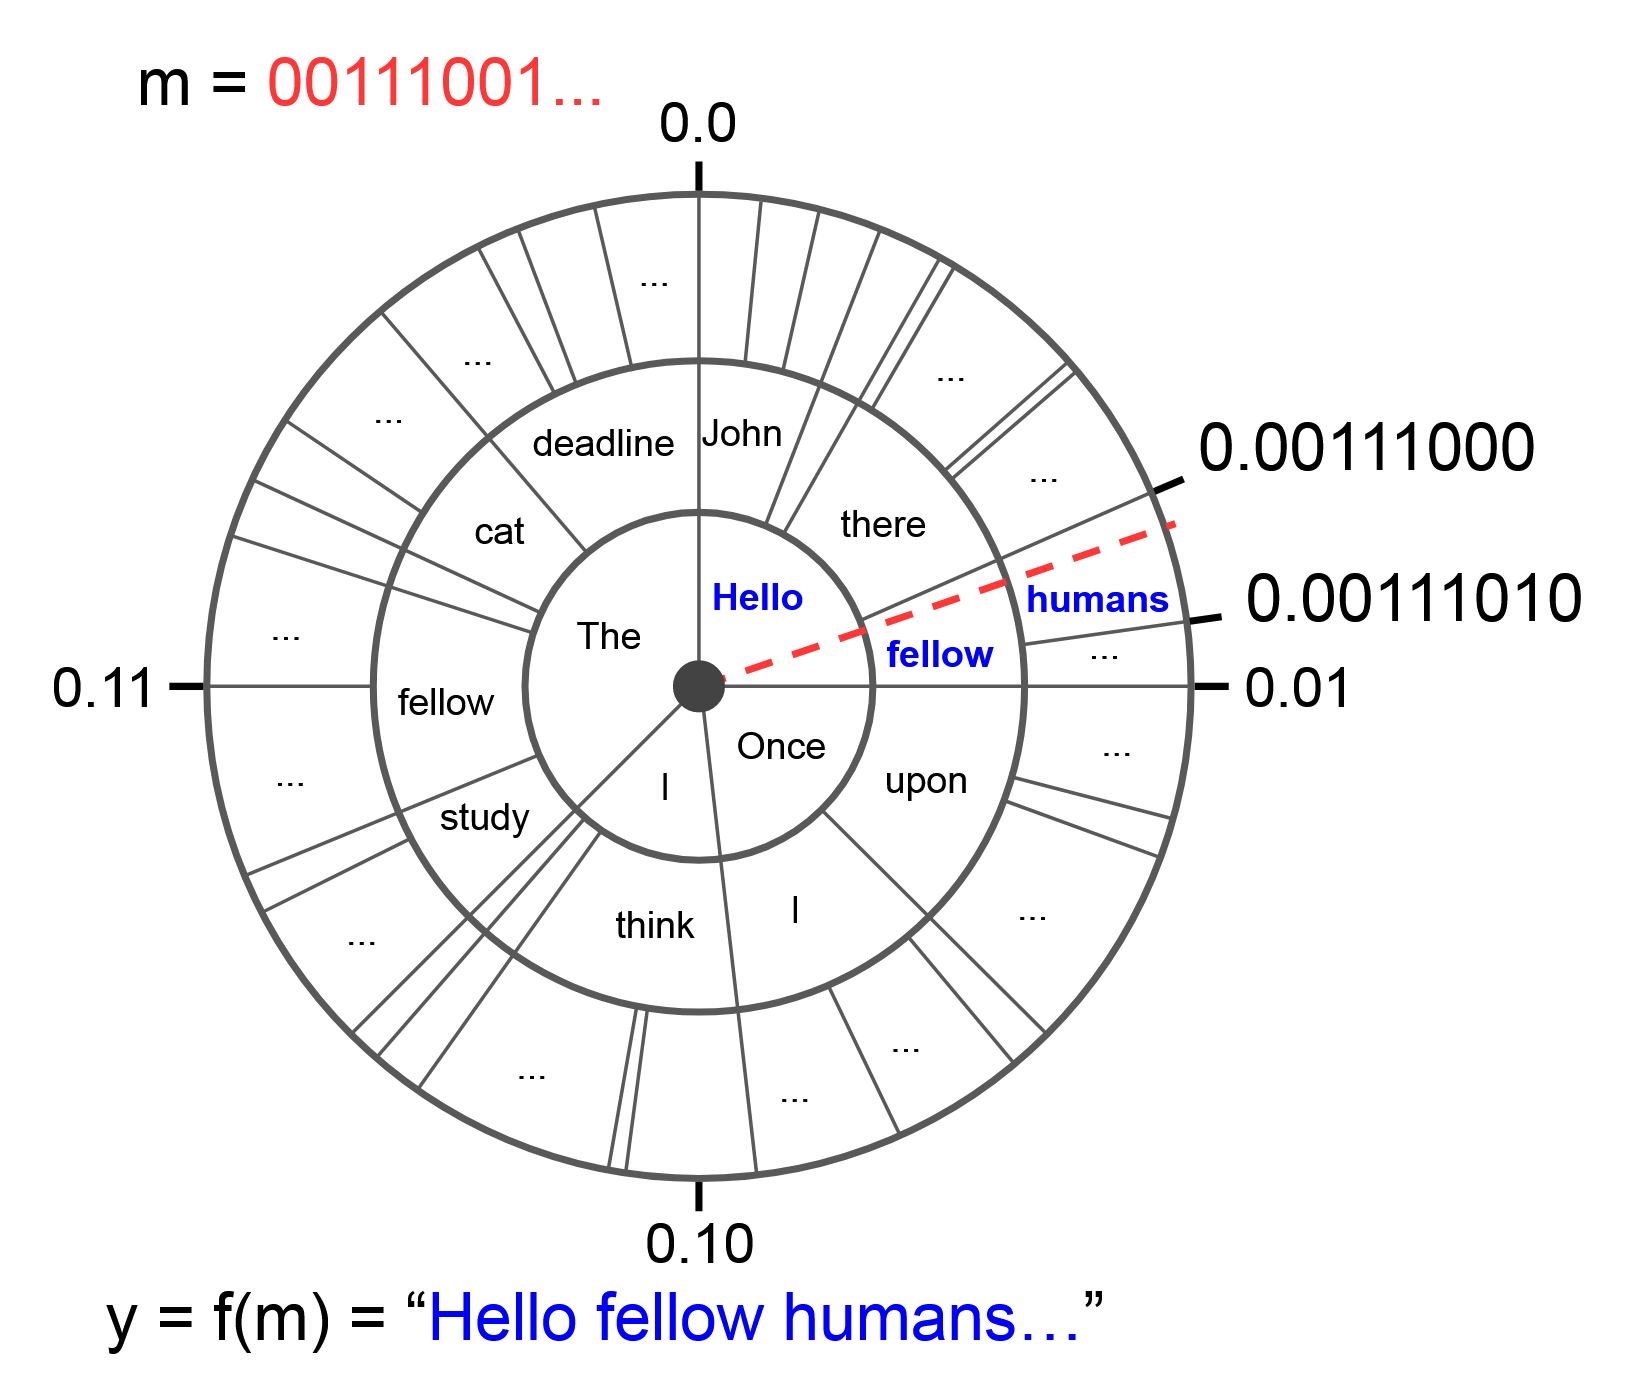
\includegraphics[width=0.75\linewidth]{arithmetic_coding.png}
		\caption[Arithmetic coding]{A visualization of Arithmetic coding. The secret message $m$ gets encoded into a cover text $y$ via a transformation $f$. Iterations are arranged as layers of a circle. The sub-intervals of $ [0, 1) $ get narrower the further they are away from the center. Taken from~\cite{zieglerNeuralLinguisticSteganography2019}.}
        \label{fig:arithmeticCoding}
    \end{wide}
\end{figure}

Arithmetic coding encodes the bits of a secret message into a cover text by sampling specific tokens. This uses the probabilities calculated by the \gls{LLM} and three parameters as input: \lstinline|temperature|, \lstinline|topK| and \lstinline|precision|. The former is a decimal number, the latter two are integers. \lstinline|topK| is a number of tokens not greater than $ n_{vocab} $, the vocabulary size of the \gls{LLM}. \lstinline|precision| is a number of bits. The output is the sampled cover text token.

First, we assign tokens to sub-intervals of an integer interval based on their cumulated probabilities: We define our initial interval as $ [0, 2^{precision}] $. We scale the probabilities by $ 1/temperature $ and sort them in descending order. We only keep the tokens with the top $ min(max(2, n), topK) $ probabilities, where $ n $ is the number of probabilities greater than the inverse width of the current interval. This cuts off any probabilities that would be rounded to zero in subsequent steps. We rescale the probabilities to the range of the current interval and round them to integers. We cumulate these integer "probabilities" for every token. As those that would be rounded to zero were cut off, every token now corresponds to a unique integer in the current interval. Interpreting these integers as upper boundaries effectively assigns every token to a sub-interval.

Then, we sample a cover text token by selecting a sub-interval based on secret message bits: In iteration $ i $, we consider the secret message bits at indices $ i $ to $ i + precision $. If there aren't enough bits left at the end, we do 0-padding. We interpret these bits as an integer and select the sub-interval this integer falls into. Thereby, we sample the token assigned to this sub-interval.

Lastly, we determine how many bits were encoded in iteration $ i $ and calculate the new interval for the next iteration: We convert the boundaries of the selected sub-interval from integer to binary and count the number of most significant bits they share as prefix. This is the number of bits that were encoded in iteration $ i $, so we increment $ i $ by this. This results in the number of most significant bits that are now fixed when representing our secret message as a number in the initial interval. This narrows our current interval down. If we use this in the next iteration, we may not have enough sub-intervals to assign tokens to. Therefore, we manipulate the selected sub-interval's boundaries so it doesn't strictly narrow down throughout iterations. We drop the fixed most significant bits from its upper and lower boundary and append as many 1s and 0s as least significant bits, respectively. Thereby, we receive the upper and lower boundary for the next iteration. This causes the boundaries to not strictly narrow down, but makes the interval as wide as possible.

The last three paragraphs show the complexity of Arithmetic coding. In particular, the interplay of the \lstinline|topK| and \lstinline|precision| parameters makes their effect on cover text quality hard to estimate. However, Arithmetic coding also comes with a significant strength. It aims to minimize \gls{KL} divergence at maximum compression, which is a measure for the divergence of the \gls{LLM}'s probability distributions with and without steganography~\cite{zieglerNeuralLinguisticSteganography2019}. The optimum of no \gls{KL} divergence can be achieved when Arithmetic coding is used with an unmodulated \gls{LLM} (i.e. \lstinline|temperature| = 1.0, \lstinline|topK| = $n_{vocab}$ and \lstinline|precision| = $ \lceil \log_2(topK) \rceil $)~\cite{zieglerNeuralLinguisticSteganography2019}. This is a powerful defense against machine-based attacks that try to identify statistical patterns in the generated cover texts~\cite{zieglerNeuralLinguisticSteganography2019}.

\subsection{Arithmetic compression}
\label{sec:arithmeticCompression}
To convert the secret message from string to binary, we implement Arithmetic compression. It repurposes the Arithmetic coding algorithm we implemented for steganography. We only focus on the relevant differences here.

The Stegasuras paper~\cite{zieglerNeuralLinguisticSteganography2019} states that Arithmetic \textit{compression} is Arithmetic \textit{decoding} of the secret message with an empty context. Inversely, it states that Arithmetic \textit{decompression} is Arithmetic \textit{encoding} with an empty context. But this is inconsistent with the Stegasuras code~\cite{zieglerHarvardnlpNeuralSteganography2025}: The context is not \textit{empty}, but consists of an end-of-generation token. With an empty context, the \gls{LLM} would not be able to generate tokens in the first place\footnote{Do not confuse "empty \lstinline|ctx|" (\cref{sec:tokenGenerationWithLlamaCpp}) with "empty context" (here). While the former refers to the \gls{LLM} being given a non-empty empty string as prompt with no prior chat history, the latter refers to the \gls{LLM} being given an empty string as prompt. Unfortunately, this ambiguity is unavoidable when sticking to the respective vocabulary of llama.cpp and Stegasuras.}. Furthermore, Arithmetic compression doesn't call the encode/decode functions with the same arguments as Arithmetic coding does: \lstinline|temperature| is fixed to 1.0, \lstinline|topK| is fixed to the vocabulary size of the \gls{LLM}, and \lstinline|precision| is set as high as possible (62 bits in our implementation). This forces the unmodulated \gls{LLM} to use as much of its vocabulary as possible in every iteration of the algorithm.

We also make some small modifications to the Arithmetic coding algorithm as implemented in Stegasuras. To clean up artefacts that may be generated during decoding of a cover text, we need to be able to sample the ASCII NUL character as a token (see \cref{sec:finishingTheLastSentence}). Arithmetic coding involves assigning tokens to sub-intervals of $ [0, 2^{precision}) $ before sampling them. To ensure that the NUL character can always be sampled, we always assign it to the last sub-interval. This is similar to more general implementations of Arithmetic compression, where the last sub-interval is interpreted as end-of-file to terminate the algorithm.

Furthermore, our implementation of Arithmetic compression comes with some overhead over the original Stegasuras implementation. As mentioned in \cref{ch:introduction}, we want to be able to encrypt the secret message bits before encoding them into a cover text. For encryption itself, a configuration such as \gls{AES} in \gls{CTR} mode would be able to simulate a stream cipher and not require any padding. But common libraries such as Android KeyStore only operate on ByteArrays, which requires us to add padding. Therefore, we prepend 0s to the binary secret message until an integer number of bytes is reached. To be able to strip the padding again during decompression, we prepend another byte that stores the number of 0s we added. This overhead is particularly relevant for short secret messages, as for example "Hello World" gets padded from 17 to 32 bits. Due to time constraints, padding was implemented, but encryption was not.

This shows some strengths and weaknesses of Arithmetic compression. Compared to UTF-8 conversion, it allows for significantly shorter cover texts. But Arithmetic compression is probabilistic. It relies on the \gls{LLM} to predict the secret message token-wise. As the secret message is arbitrary user input, the \gls{LLM} may not be able to predict it. This makes Arithmetic compression slightly prone to failures. However, Arithmetic compression doesn't need to store any metadata about the secret message to be able to decompress it again. This is a benefit over many other compression algorithms~\cite{huffmanMethodConstructionMinimumRedundancy1952}, as it significantly reduces attack surface.

\section{Creating a conversation between cover texts}
\label{sec:creatingAConversationBetweenCoverTexts}
A \gls{LLM} fundamentally works by completing any prompt it is given (see \cref{sec:tokenGenerationWithLlamaCpp}). We are already able to leverage this for steganography by manipulating token generation, thereby encoding a secret message into a cover text (see \cref{sec:steganographyEncodingDecoding}). But we still don't have a way to create a conversation between cover texts. This means our first requirement (see \cref{ch:introduction}) is not fulfilled yet.

This section will show how creating a conversation between cover texts is possible. We will also show how to influence the \gls{LLM} behaviour on a lower level, via a system prompt. Both is achieved at once, by formatting the context as a conversation using special tokens~\cite{jiangChatBugCommonVulnerability2025}.

The context is formatted into a conversation by structuring it into messages. Each message has a role and a content~\cite{jiangChatBugCommonVulnerability2025}. There are three possible roles: System, user and assistant~\cite{jiangChatBugCommonVulnerability2025}. The system role is reserved for the system prompt. Its content is a natural language command the user can give the \gls{LLM} to influence its behaviour~\cite{jiangChatBugCommonVulnerability2025}. For the \gls{LLM}, the system prompt is always the first message of the conversation. In a typical \gls{UI} however, the system prompt is hidden away in the settings. Our implementation handles it like this too.

The user role is assigned to the subsequent prompts input by the user~\cite{jiangChatBugCommonVulnerability2025}. The assistant role is assigned to the responses output by the \gls{LLM}~\cite{jiangChatBugCommonVulnerability2025}. At the end of the formatted context, the special token for the assistant role is appended. This signals the \gls{LLM} to continue the conversation, i.e. to respond to the last message. Listing~\ref{lst:chatTemplate} shows an example.

% Add some space on top of listing to match bottom
\vspace{0.25cm}

\begin{lstlisting}[caption={[llama.cpp: Chat templates]{Example for a context formatted with the chat template of Llama 3.2 1B. Some line breaks have been added for readability.}}, label={lst:chatTemplate}]
<|start_header_id|>system<|end_header_id|>Let's do a role play. You and I are friends, texting with each other. We talk about what we did on the weekend. Be brief and casual, but friendly and engaging. Use emojis and phrases typical for chat messages.<|eot_id|>
<|start_header_id|>user<|end_header_id|>How was your weekend?<|eot_id|>
<|start_header_id|>assistant<|end_header_id|>
\end{lstlisting}

Unfortunately, the special tokens for context formatting are not uniform across \glspl{LLM}. Fortunately, llama.cpp has support for a wide range of formattings. In the vocabulary of llama.cpp, they are called chat templates~\cite{gerganovGgerganovLlamacpp2024,jiangChatBugCommonVulnerability2025}. We can query a \gls{LLM} for its chat template and pass this as a parameter to other functions. Thereby, we remain compliant with our fourth requirement of making the \gls{LLM} swappable (see \cref{ch:introduction}).

When completing the formatted context, the \gls{LLM} performs our algorithm-specific sampling (see \cref{sec:algorithms}). In doing so, we encode information in the next chat message and create a conversation from cover texts. Finally, our first requirement is fulfilled.

Strictly speaking, the conversation doesn't need to consist only of \textit{cover texts}. It may as well be composed of an arbitrary mixture of cover texts and plain texts, i.e. messages that don't encode a secret message. Our app allows this by letting the user toggle steganography on/off on the conversation screen (see \cref{sec:conversationScreen}). This gives the user great freedom to steer the topic of the conversation by sending plain text messages for non-sensitive communication. In addition to the system prompt, this enables us to improve cover text quality further.

Lastly, we mentioned that the \gls{LLM} needs to be able to talk \textit{to itself} (see \cref{sec:howToSelectASuitableLLM}). What we mean by this is that the \gls{LLM} is used by both chat partners to generate cover texts that are replies to the other chat partner. Consider this example: We have two chat partners, Alice and Bob. Alice wants to send a new cover text to Bob. The prior messages in the conversation are used as context. For encoding, Alice's prior messages have to be assigned the assistant role and Bob's prior messages have to be assigned the user role. When Bob receives this cover text, he has to replicate this state to decode it. When Bob wants to reply with another cover text, the roles are inversed. For encoding, Bob's prior messages have to be assigned the assistant role and Alice's prior messages have to be assigned the user role. Alice has to replicate this state to decode it. The roles are constantly switched following this pattern, effectively making the \gls{LLM} talk to itself without knowing it.

\section{Emojis}
\label{sec:emojis}
Emojis are widely used in instant messaging to express emotions, add visualizations or draw attention~\cite{zhouGoodbyeTextHello2017}. Being able to enrich our cover texts with this form of non-verbal communication is essential to make them seem organic. Today's \glspl{LLM} are able to output emojis when being prompted to (see \cref{sec:howToSelectASuitableLLM}). By demanding emojis in the system prompt, our app is able to do this as well. Accomplishing this however required some attention to detail. Therefore, we explain what needs to be considered when working with emojis and other non-ASCII characters in the context of the \gls{JNI} (see \cref{sec:javaNativeInterface}).

The \gls{JNI} is used to pass parameters between our Kotlin and C++ code. This requires conversions between the corresponding data types. For most data types this is simple, but for strings this is more sophisticated. This is due to collisions between different character encodings. As the ASCII encoding is contained in virtually all other encodings, pure ASCII strings generally are interoperable~\cite{gleaveMakingCompressionAlgorithms2017}. While the ASCII character set is sufficient for basic communication in English, it doesn't include emojis.

Emojis require the full Unicode character set. This can be encoded in various ways, the most common being UTF-8~\cite{gleaveMakingCompressionAlgorithms2017}. Consider the implementation of the \lstinline|LlamaCpp.detokenize| function in our source code: It detokenizes an array of token IDs back into a string using the \gls{JNI}. On the C++ side, one might be tempted call the \lstinline|NewStringUTF| function to create a \lstinline|jstring| object to pass back to Kotlin. While this works fine for ASCII strings, it makes our app crash when working with emojis. This is due to a \textit{modified} UTF-8 encoding being used by Java and therefore by the \gls{JNI}~\cite{oracleJNIFunctions}. To bypass this, we return the UTF-8 encoding of a string as a \lstinline|jbyteArray| instead. On the Kotlin side, we explicitly call the String constructor to specify that the bytes are UTF-8. This abstracts any Kotlin internals away.

While emojis now enable us to improve cover text quality, they introduce some further difficulties. When finishing the last sentence of the cover text during encoding, we use greedy sampling and terminate when reaching a suitable punctuation mark (see \cref{sec:finishingTheLastSentence}). To fulfill the third requirement defined in \cref{ch:introduction}, we have to keep cover texts as short as possible. If a cover text contains emojis, they may be used in place of punctuation marks to end a sentence~\cite{zhouGoodbyeTextHello2017}. But unlike punctuation marks, emojis cannot easily be detected using the Kotlin standard library. A simple approach like detecting non-ASCII characters would already conflict with the German letters ä, ö and ü, for example. A more sophisticated approach was implemented, using regular expressions to detect the Unicode categories containing emojis. But this didn't yield satisfying results as it corrupted a significant portion of cover texts. Therefore, cover texts including emojis only end when an appropriate punctuation mark is generated. This possibly makes them longer than necessary. But we consider it worth the trade-off, as the use of emojis can be easily influenced via the system prompt.

% !TeX root = ../Thesis.tex

%************************************************
\chapter{Evaluation}\label{ch:evaluation}
%************************************************
\glsresetall % Resets all acronyms to not used

We perform both quantitative and qualitative evaluation to assess how well our implementation fulfills the requirements we set ourselves in \cref{ch:introduction}. This allows for a comprehensive judgement of what future development of \gls{HiPS} should focus on.

\section{Recommended settings}
\label{sec:recommendedSettings}
For our evaluation to be exhaustive, we would have to test a plethora of available hardware and software configurations. Since this is not feasible, we focus on entry-level smartphones and recommended settings. Thereby, we assume the lowest common denominator in hardware. We expect this to give us a good estimate of how useful our app would be in the real world. Both quantitative and qualitative evaluation is done on the smartphones listed in \cref{tab:smartphones} earlier, using our \gls{LLM} of choice, Llama 3.2 1B.

Similarly, we focus on running the steganography algorithms with our recommended settings: For Arithmetic coding, we recommend \lstinline|temperature| = 1.0, \lstinline|topK| = 128,256 tokens (the \gls{LLM}'s vocabulary size) and \lstinline|precision| = $ \lceil \log_2(topK) \rceil $ = 17 bits. This is based on the results of Stegasuras, which showed that Arithmetic coding can achieve the optimum of no \gls{KL} divergence with an unmodulated \gls{LLM}~\cite{zieglerNeuralLinguisticSteganography2019}. For Huffman coding, we recommend \lstinline|bitsPerToken| = 2 bits/token. This is because in our subjective judgement, it offers the best trade-off between cover text quality and length. Quality is similar to \lstinline|bitsPerToken| = 1 at twice the efficiency, making cover texts 50\% shorter. With \lstinline|bitsPerToken| = 3, quality degrades significantly, starting diminishing returns for savings in length. Arithmetic compression is recommended in any case. Lastly, we recommend the context length to be 2 messages. This is because in our subjective judgement, cover text quality was sufficient while computational costs can nearly be minimized with this setting.

\section{Quantitative evaluation}
\label{sec:quantitativeEvaluation}
Quantitative evaluation of our app focusses on three dimensions: Performance, efficiency and reliability. We measure performance as the speed of token generation, efficiency as the ratio of Arithmetic compression over UTF-8, and reliability as the success rate of cover text decoding. All three are crucial factors for gaining acceptance amongst users.

\subsection{Performance}
\label{sec:performance}
To appeal to a large user base, we set ourselves the requirement of acceptable performance on entry-level devices. We measure performance via the speed of token generation, as this is the main task of our app. \cref{tab:performance} shows the encoding and decoding speeds we achieved for every combination of smartphone and algorithm. The speeds were averaged over a conversation of ten cover texts, each encoding a random sentence of up to five words as secret message. With both of our entry-level devices measuring at around 1 token/second, user experience is smooth enough to fulfill our requirement.

\begin{table}
	\centering
	\begin{tabular}{@{} lrr @{}} % @{} removes white spaces
		\toprule
		\tableheadline{Device} & \tableheadline{Encoding} & \tableheadline{Decoding} \\
		\midrule
        Arithmetic               &                 &                 \\
		\midrule
        Moto One Vision          & $1.24 \pm 0.21$ & $1.26 \pm 0.21$ \\
		Moto E13                 & $0.95 \pm 0.11$ & $0.95 \pm 0.11$ \\
        Samsung Galaxy S24 Ultra & $3.59 \pm 0.40$ & $3.54 \pm 0.38$ \\
        \midrule
        Huffman                  &                 &                 \\
        \midrule
        Moto One Vision          & $1.24 \pm 0.15$ & $1.26 \pm 0.17$ \\
		Moto E13                 & $0.92 \pm 0.08$ & $0.92 \pm 0.09$ \\
        Samsung Galaxy S24 Ultra & $3.44 \pm 0.49$ & $3.27 \pm 0.50$ \\
		\bottomrule
	\end{tabular}
	% Use alternative short title for table of contents
	\caption[Performance measurements]{Average encoding and decoding speeds and their standard deviations for every combination of smartphone and algorithm. All values are measured in tokens/second.}
	\label{tab:performance}
\end{table}

However, our implementation shows a considerable performance deficit in comparison to other apps running \glspl{LLM} with llama.cpp: In \cref{sec:howToRunLLMsOnAndroid}, we found that we can achieve around to 5 tokens/second on the same smartphones. Overhead is similar on our flagship device, which achieved up to 4 tokens/second with our app versus up to 25 tokens/second with the other apps. This is likely because the other implementations we investigated perform token sampling in C++ rather than Kotlin. Therefore, they don't have to pass data through the \gls{JNI} for every token. We underestimated the impact of this design decision in the early phases of development due to lack of experience.

\subsection{Corrupted cover texts}
\label{sec:corruptedCoverTexts}
Due to the probabilistic nature of \glspl{LLM}, the responses they generate are hard to predict. But as \glspl{LLM} are stateless, their responses to a given prompt should be reproducible (see \cref{sec:tokenGenerationWithLlamaCpp} for details). In particular, this should apply to the cover text tokens generated during steganographic encoding and decoding. In our testing, we encountered some issues with this. While the vast majority of cover texts could be decoded, some were corrupted: For these cover texts, the token predictions of the \gls{LLM} were inconsistent between encoding and decoding. This renders the encoded secret messages unrecoverable.

To quantify this, we generated ten conversations of ten cover texts. Each cover text encoded a random sentence of up to five words as secret message. Each conversation was given a different system prompt. We did this for both algorithms, using the recommended settings defined earlier. Arithmetic coding was able to decode 98 out of the 100 cover texts, Huffman coding achieved 97 out of 100.

While this is robust enough for a demonstration, it should be investigated further to make \gls{HiPS} ready for production. Stegasuras already mentions that this issue may be related to the use of tokenization based on \gls{BPE}~\cite{zieglerStegasuras2025}. While Stegasuras already implements some fixes~\cite{zieglerHarvardnlpNeuralSteganography2025}, translating them to our implementation could not resolve the issue reliably. Future research may also investigate how significant this is when using larger, less quantized \glspl{LLM}, as those supposedly are more accurate. Users can however already bypass the issue in most cases by simply sending an affected secret message again, so that it gets encoded it with a different context.

\section{Qualitative evaluation}
\label{sec:qualitativeEvaluation}
Our implementation of steganography is based on Stegasuras~\cite{zieglerNeuralLinguisticSteganography2019}, but our approach for qualitative steganalysis differs. We evaluate robustness of our cover texts against human eavesdroppers via a survey.

\subsection{Survey design}
\label{sec:surveyDesign}
Stegasuras performed qualitative steganalysis by letting humans judge if a given sentence was a plausible continuation of a given context taken from a news article (see \cref{sec:lowLevelManipulatingTokenGeneration}). While such an approach would allow us to calculate a success rate for fooling humans with our cover texts, its applicability is limited. Stegasuras already mentions that a head-to-head comparison of two possible continuations of the same context is uncommon in everyday life~\cite{zieglerNeuralLinguisticSteganography2019}. Our use case of creating chat conversations from cover texts introduces further limitations. While the plausibility of news articles can be judged by their factual accuracy~\cite{zieglerNeuralLinguisticSteganography2019}, chat messages often don't contain objectively verifiable claims. Instead, they regularly contain personal information that is only verifiable by the people chatting with each other.

Therefore, we chose to evaluate to what extent our cover texts fulfill certain linguistic characteristics typically found in chat messages. As such characteristics are largely influenced by the system prompt (see \cref{sec:creatingAConversationBetweenCoverTexts}), we expect this approach to give us insights in how to refine it further. A study among Canadian university students serves as a framework~\cite{alazzawieLinguisticSituationalFeatures2022}, as the audience for our survey is expected to be similar (i.e. students of TU Darmstadt). We summarize the characteristics found in this framework as follows: Use of correct grammar/spelling, use of emojis, and use of abbreviations. We added the length of chat messages as a new characteristic. This helps us understand how significant the compression overhead of our implementation is. We use a 5-point Likert scale~\cite{likertTechniqueMeasurementAttitudes1932} for each of the four characteristics. As Likert scales are a widely used method for gathering user feedback in software development, we expect participants to quickly be familiar with them~\cite{girayAssessmentStudentSatisfaction2021,tizardVoiceUsersExtended2022}.

We presented participants of our survey with screenshots of six chat conversations: Four were cover texts generated by the \gls{LLM} (two for each algorithm), two were real (donated by members of the SEEMOO group). We generated cover texts by encoding random sentences of up to five words with system prompts similar to the example shown in \cref{fig:lmStudio}. \cref{ch:survey} contains all chat conversations we used, both real and cover texts, and the system prompts corresponding to the cover texts. We asked participants to rate how similar these conversations are to their own messages using the Likert scales (e.g. "I use emojis in a similar way" from 1 = "Strongly disagree" to 5 = "Strongly agree"). We also gave them the option to add comments to explain their ratings for each conversation. Participants did not know any of the conversations were generated by a \gls{LLM}, as we presented the survey to be about linguistics rather than steganography.

\subsection{Survey results}
\label{sec:surveyResults}
Our survey delivered valuable insights in how to increase cover text quality further. \cref{fig:likertplots} shows an overview of the results. Participants generally rated the real conversations as more similar to their own chats than the cover texts. Cover texts were rated the most dissimilar in the use of emojis. This is explained in the comments ten participants gave: The \gls{LLM} tends to use emojis rather mechanically. For example, "I'm running late" may be followed by a clock emoji. Instead of enriching cover texts with non-verbal communication by expressing emotions, this only reiterates what is already being said.

\begin{figure}
    \begin{wide}
        \centering
        \captionsetup{width=\linewidth}
        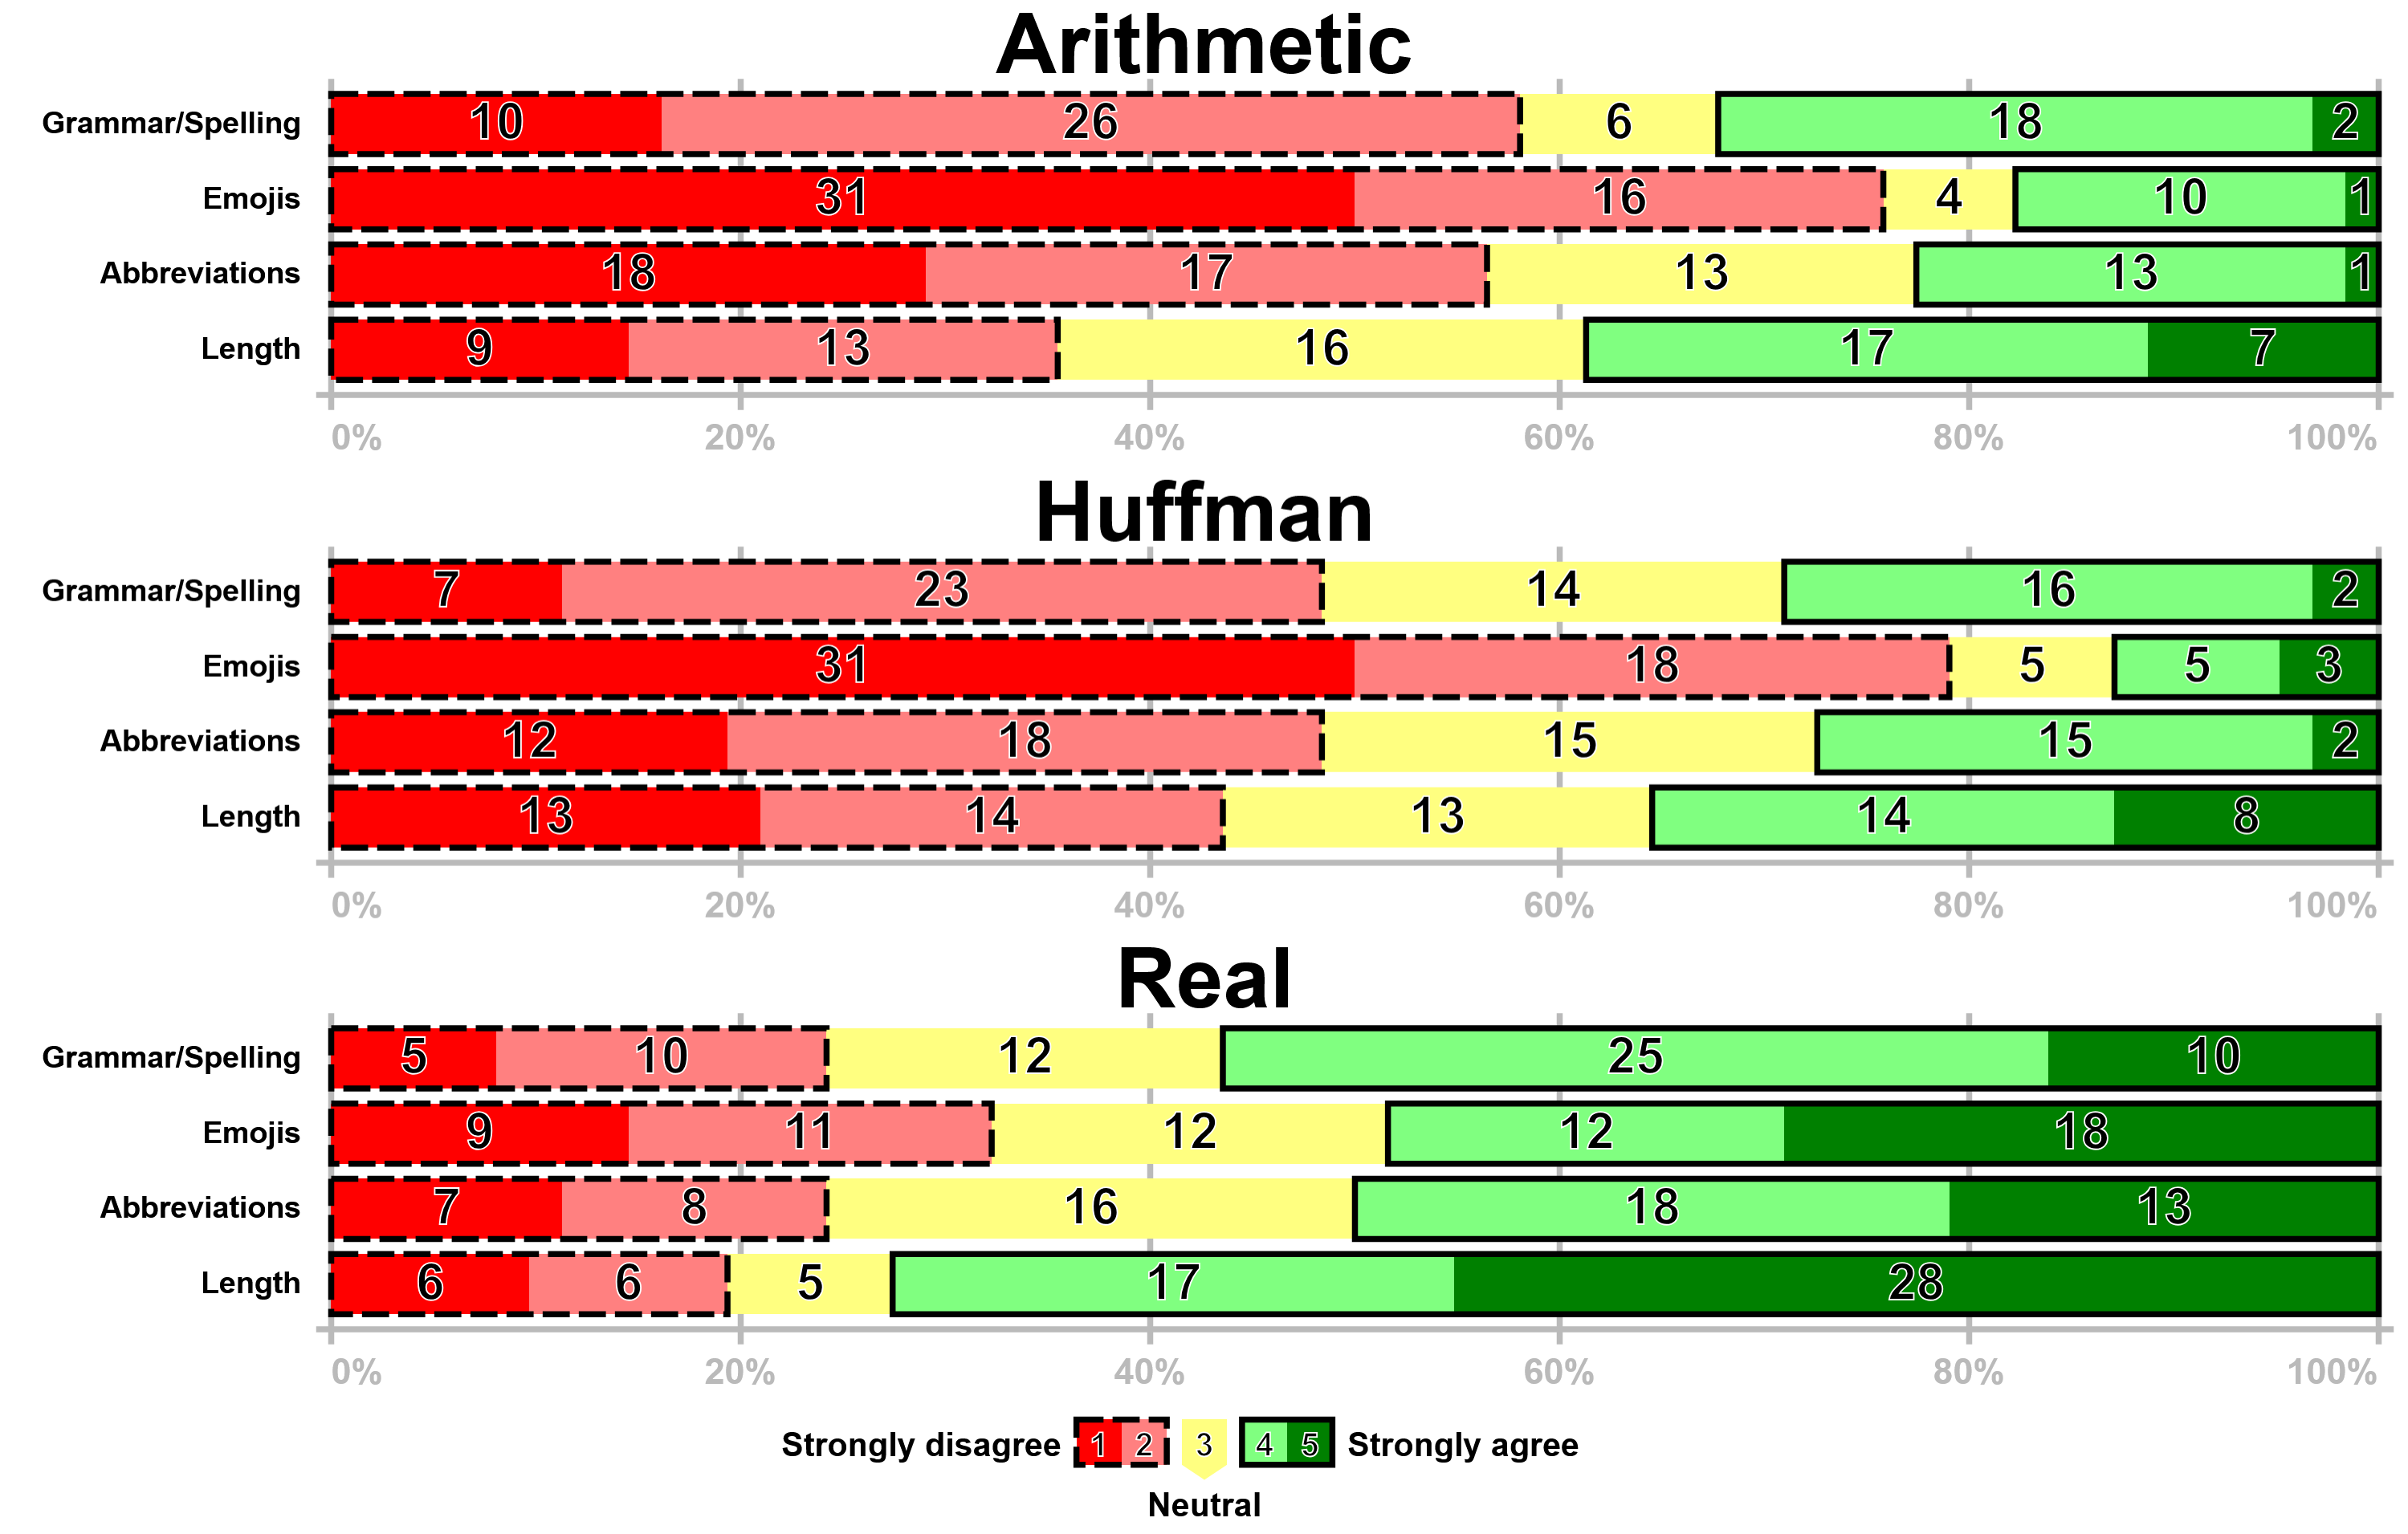
\includegraphics[width=\linewidth]{likertplots.png}
        \caption[Survey: Results]{Survey results. Similarity ratings on the Likert scales have been aggregated for cover texts generated with Arithmetic coding, Huffman coding and real messages, respectively.}
        \label{fig:likertplots}
    \end{wide}
\end{figure}

Higher similarity was achieved in the use of grammar/spelling and abbreviations. Participants expressed various personal preferences regarding the use of specific emojis and abbreviations. Furthermore, four participants commented that they don't include interjections or sounds (e.g. "oh", "ugh") in their messages, which our \gls{LLM} tends to do. Training a \gls{LLM} on one's own chat messages as demonstrated in~\cite{donnerSimulationMeFinetuning2024} may therefore be promising. Message length was rated the most similar. This implies that users of our app would have to restrict themselves to secret messages of around five words to generate plausible cover texts.

Overall, this survey highlights the variety with which our chat messages reflect our personalities. Anecdotally, seven participants commented that either they or someone they know write messages similar to our cover texts, while two other participants commented that the same cover texts look like they were generated by \gls{AI}. One participant commented that our cover texts were typical for older people, who may write more formal messages like pen pals, as opposed to younger people, who may be more chaotic in their communication. As our participants were mostly students of TU Darmstadt, they belong to a relatively young demographic. This may have introduced a bias in our survey. The study we use as framework (see \cref{sec:surveyDesign}) supports this by suggesting that there may be two kinds of users, divided by writing more functional versus more elaborate messages~\cite{alazzawieLinguisticSituationalFeatures2022}. Repeating this survey while targeting an older demographic could therefore be promising.

\subsection{Demographic limitations and randomization}
\label{sec:demographicLimitationsAndRandomization}
With 31 participants, our survey is not representative. It is specific to our choice of \gls{LLM}, system prompts, recommended settings and demographic of participants: While the former three are already explained in \cref{sec:howToSelectASuitableLLM,sec:recommendedSettings}, the latter still needs to be discussed. In addition to rating linguistic characteristics, we also asked participants for their age range and native language. All participants were German-speakers in the two youngest age ranges (18-24 and 25-34), which is to be expected with students of TU Darmstadt. Due to the limited ability of small \glspl{LLM} to speak languages other than English, participants were presented English conversations. As our audience has a scientific background, we deemed this acceptable.

Lastly, randomization is limited further by the small number of conversations. This is due to the lack of publicly available datasets of organic chat messages. Datasets from adjacent fields (e.g. Reddit comments~\cite{baumgartnerPushshiftRedditDataset2020} or Telegram channels~\cite{morgiaTGDatasetCollectingExploring2025}) were not used as they mostly don't follow a dialogue structure.

\iftoggle{parts}{
	\cleardoublepage
	\ctparttext{After the evaluation, we further discuss the results and give an outlook. In addition, we finish this work with conclusions.}
	\partExtra{Discussion and Conclusions}
}{}
% !TeX root = ../Thesis.tex

%************************************************
\chapter{Discussion}\label{ch:discussion} % $\mathbb{ZNR}$
%************************************************
\glsresetall % Resets all acronyms to not used

\lipsum[6]

% !TeX root = ../Thesis.tex

%************************************************
\chapter{Conclusions}\label{ch:conclusions}
%************************************************
\glsresetall % Resets all acronyms to not used

\lipsum[7]



% ------------------------------------------------------------------
% Backmatter
% ------------------------------------------------------------------
\iftoggle{parts}{}{
	\addtocontents{toc}{\protect\vspace{\beforebibskip}} % add space between main chapters and appendix if we do not use parts
}
\appendix
\cleardoublepage
\iftoggle{parts}{
	\partExtra{Appendix}
}{}
% !TeX root = ../Thesis.tex

%********************************************************************
% Some Proof (Appendix)
%*******************************************************
% -- TemplateKnob
% If problems with the headers: get headings in appendix etc. right
%\markboth{\spacedlowsmallcaps{Appendix}}{\spacedlowsmallcaps{Appendix}}
\chapter{Some Proof}\label{ch:SomeProof}
\glsresetall % Resets all acronyms to not used



% ------------------------------------------------------------------
% Other Stuff in the Back
% ------------------------------------------------------------------
\iftoggle{parts}{
	% !TeX root = ../Thesis.tex

\pdfbookmark[-1]{Back Matter}{backmatter}

}{}
\cleardoublepage% !TeX root = ../Thesis.tex

%********************************************************************
% Bibliography
%*******************************************************
% work-around to have small caps also here in the headline
% https://tex.stackexchange.com/questions/188126/wrong-header-in-bibliography-classicthesis
% Thanks to Enrico Gregorio
\defbibheading{bibintoc}[\bibname]{%
  \phantomsection
  \manualmark
  \markboth{\spacedlowsmallcaps{#1}}{\spacedlowsmallcaps{#1}}%
  \addtocontents{toc}{\protect\vspace{\beforebibskip}}%
  \addcontentsline{toc}{chapter}{\texorpdfstring{\tocEntry{#1}}{#1}}%
  \chapter*{#1}%
}
\printbibliography[heading=bibintoc]

% !TeX root = ../Thesis.tex

%*******************************************************
% AI Declaration
%*******************************************************

% Adjust this text as necessary.
% NOTE: If you use AI for more things, you have to explicitly acknowledge this. See: https://www.informatik.tu-darmstadt.de/media/informatik/fb20_studium/infos_dozenten/20240126_KI_Hilfsmittel.de.pdf

\chapterExtra{AI Declaration}
This thesis was written independently and was linguistically revised with the help of Llama 3.3 70B via \url{https://duck.ai}.

\iftoggle{phd}{
	% -- TemplateKnob
	%\cleardoublepage% !TeX root = ../Thesis.tex

%************************************************
\chapterExtra{Curriculum Vit\ae}\label{ch:CurriculumVitae}
%************************************************

\begin{cv}{}

\renewcommand*{\cvlistheadingfont}{\spacedlowsmallcaps} % same as sections
\renewcommand*{\cvlabelfont}{\itshape}
\setlength\cvlabelwidth{60pt}

\begin{cvlist}{{Personal Information}}
    \item[Name] \myName
    \item[Date of Birth] \myBirthDate
    \item[Place of Birth] \myBirthPlace
    \item[Nationality] \myNationality
\end{cvlist}


\begin{cvlist}{{Education}}

\item[since 2018] \textbf{Doctoral Candidate} \\
Computer Science, Technische Universiät Darmstadt, Darmstadt, Germany

\item[2016--2018] \textbf{Master of Science} \\
Computer Science, Technische Universität Darmstadt, Darmstadt, Germany

\item[2013--2016] \textbf{Bachelor of Science} \\
Computer Science, Technische Universität Darmstadt, Darmstadt, Germany

\end{cvlist}


\begin{cvlist}{{Work Experience}}

\item[since 2012] \textbf{Research Associate} \\
Secure Mobile Networking Lab, Technische Universität Darmstadt, Darmstadt, Germany.

\end{cvlist}


\begin{cvlist}{{Awards}}

\item[Publication] \textbf{Best Community Paper Award at ACM MobiCom '18} \\
Paper: \enquote{One Billion Apples’ Secret Sauce: Recipe for the Apple Wireless Direct Link Ad hoc Protocol}.

\end{cvlist}        


\begin{cvlist}{{Supervised Student Theses}}

\item[B.\,Sc. Thesis] \textbf{Another Student}, \enquote{A Very Cool Topic}, 2018.

\item[M.\,Sc. Thesis] \textbf{Milan Schmittner}, \enquote{Scalable and Secure Multicast Routing for Mobile Ad-hoc Networks}, 2014.

\end{cvlist}

% -- TemplateKnob
% \begin{cvlist}{{Miscellaneous}}
% \item[Teaching] Organization of the integrated course \enquote{Network Security}.
% \end{cvlist}


\date{\myLocation{}, \myTime{}}

\end{cv}
 % not required in final submission
	\cleardoublepage%!TEX root = ../Thesis.tex

\begin{otherlanguage}{ngerman}

%*******************************************************
\chapterExtra{Erklärung zur Dissertationsschrift}
%*******************************************************

% Promotionsordnung und mehr des FB 20
% https://www.informatik.tu-darmstadt.de/forschung_fb20/wissenschaftliche_karriere/promotion/index.de.jsp

\begin{flushright}
    \emph{\small gemäß §\,9 der Allgemeinen Bestimmungen der Promotionsordnung der \\
    Technischen Universität Darmstadt vom \formatdate{12}{1}{1990} (ABI. 1990, S.\,658) \\
    in der Fassung der 8.\,Novelle vom \formatdate{1}{3}{2018}}
\end{flushright}
Hiermit versichere ich, \myName{}, die vorliegende Dissertationsschrift ohne Hilfe Dritter und nur mit den angegebenen Quellen und Hilfsmitteln angefertigt zu haben. Alle Stellen, die Quellen entnommen wurden, sind als solche kenntlich gemacht. Eigenzitate aus vorausgehenden wissenschaftlichen Veröffentlichungen sowie die Urheberschaften der einzelnen Beiträge sind in Anlehnung an die Hinweise des Promotionsausschusses des Fachbereichs Informatik zum Thema \enquote{Kumulative Dissertation und Eigenzitate in Dissertationen} (CR; 01.12.2022) im Kapitel \enquote{\emph{Collaborations and My Contribution}} auf den \cpagerefrange*{ch:Collaborations}{ch:CollaborationsEnd} angegeben. Diese Arbeit hat in gleicher oder ähnlicher Form noch keiner Prüfungsbehörde vorgelegen. In der abgegebenen Dissertationsschrift stimmen die schriftliche und die elektronische Fassung überein.
% cannot use \nameref for chapter name, see
% https://bitbucket.org/amiede/classicthesis/issues/170/nameref-for-chapter-showing-the-previous

\bigskip

\noindent\textit{\myLocation{}, \myTime{}}

\begin{flushright}
    \begin{tabular}{m{5cm}}
        \\ \hline
        \centering\myName{} \\
    \end{tabular}
\end{flushright}

\end{otherlanguage}

}{
	\cleardoublepage% !TeX root = ../Thesis.tex

%*******************************************************
% Declaration
%*******************************************************

% Text aus: https://www.intern.tu-darmstadt.de/media/dezernat_ii/referat_iig/formulare_vorlagen/pm_1/erklaerungen/Erklaerung_zur_Abschlussarbeit_Vorlage.docx
% Stand: 3. Juni 2019

\begingroup

\begin{otherlanguage}{ngerman}
\chapterExtra{Erklärung zur Abschlussarbeit}
\begin{flushright}
	\emph{gemäß §\,22 Abs.\,7 und §\,23 Abs.\,7 APB TU Darmstadt}
\end{flushright}
Hiermit versichere ich, \myName{}, die vorliegende \myDegree{} gemäß §\,22 Abs.\,7 APB der TU Darmstadt ohne Hilfe Dritter und nur mit den angegebenen Quellen und Hilfsmitteln angefertigt zu haben. Alle Stellen, die Quellen entnommen wurden, sind als solche kenntlich gemacht. Diese Arbeit hat in gleicher oder ähnlicher Form noch keiner Prüfungsbehörde vorgelegen.
Mir ist bekannt, dass im Falle eines Plagiats (§\,38 Abs.\,2 APB) ein Täuschungsversuch vorliegt, der dazu führt, dass die Arbeit mit 5,0 bewertet und damit ein Prüfungsversuch verbraucht wird. Abschlussarbeiten dürfen nur einmal wiederholt werden.
Bei der abgegebenen Thesis stimmen die schriftliche und die zur Archivierung eingereichte elektronische Fassung gemäß §\,23 Abs.\,7 APB überein.
\end{otherlanguage}

\vfill

\let\cleardoublepage\relax
\chapter*{Thesis Statement}
\begin{flushright}
	\emph{pursuant to §\,22 paragraph 7 and §\,23 paragraph 7 of APB TU Darmstadt}
\end{flushright}

I herewith formally declare that I, \myName{}, have written the submitted \myDegree{} independently pursuant to §\,22 paragraph 7 of APB TU Darmstadt. I did not use any outside support except for the quoted literature and other sources mentioned in the paper. I clearly marked and separately listed all of the literature and all of the other sources which I employed when producing this academic work, either literally or in content. This thesis has not been handed in or published before in the same or similar form.
I am aware, that in case of an attempt at deception based on plagiarism (§\,38 paragraph 2 APB), the thesis would be graded with 5.0 and counted as one failed examination attempt. The thesis may only be repeated once.
In the submitted thesis the written copies and the electronic version for archiving are pursuant to §\,23 paragraph 7 of APB identical in content.

\vfill

\noindent\textit{\myLocation{}, \myTime{}}

\begin{flushright}
    \begin{tabular}{m{5cm}}
        \\ \hline
        \centering\myName{} \\
    \end{tabular}
\end{flushright}

\endgroup

}


% ------------------------------------------------------------------
% Game Over: Restore, Restart, or Quit?
% ------------------------------------------------------------------
\end{document}